\documentclass[
	printed,
	twoside,
	color,
	table,
	nolot,
	nolof,
	cover
	%nocover
]{fithesis3}

% load init of fithesis macros
\thesissetup{
	title 		= {
		Deep learning in cryptography
	},
	author 		= Bc. Radovan Lap\'{a}r,
	keywords 	= {RSA, cryptography, neural networks, deep learning, metacentrum},
	advisor 	= {doc. RNDr. Tomáš Brázdil, Ph.D.},
	gender 		= m,
	type 		= mgr,
	faculty 	= fi,
	% assignment 	= {./zadanie.pdf, ./prehlasenie.pdf}
}

\thesislong{abstract} {This thesis focuses on the study of deep learning in cryptography. It includes the analysis of more than 20 different sources of RSA cryptographic libraries and cards and the bias introduced in the process of primes generation. It presents the flow of working with given dataset and implements two different classifiers, which are then compared to the traditional methods already used in the field.}

\thesislong{thanks} {I would like to thank my supervisor doc. RNDr. Tomáš Brázdil, Ph.D. for his guidance and advice in the field. Moreover, I would like to thank RNDr. Petr Švenda, Ph.D. and RNDr. Matúš Nemec from the CROCS lab for the consultations and assistance during the whole process.}


% load custom packages
\usepackage{packages}

% apply fithesis styles now, so we can modify some of them before \begin{document}
\thesisload

% custom hyphenations
% \hyphenation{con-sis-ten-cy}

\makeatletter

% makes subsubsections italic
% makes smaller spaces between and after the subsubsection header
% \renewcommand\subsubsection{%
% 	\@startsection{subsubsection}{3}{\z@}{%
%   	-2.25ex plus-1ex minus-.2ex}{0.6ex plus.2ex}{%
% 	\reset@font\normalsize\it}
%}

%remove vertical spaces between chapters in table of contents	
% \renewcommand*\l@chapter[2]{%
% 	\ifnum \c@tocdepth >0\relax
% 	\addpenalty{-\@highpenalty}%
% 	%\addvspace{1.0em \@plus\p@}%
% 	\setlength\@tempdima{1.5em}%
% 	\begingroup
% 	\parindent \z@ \rightskip \@pnumwidth
% 	\parfillskip -\@pnumwidth
% 	\leavevmode \bfseries
% 	\advance\leftskip\@tempdima
% 	\hskip -\leftskip
% 	#1\nobreak\hfil \nobreak\hb@xt@\@pnumwidth{\hss #2}\par
% 	\penalty\@highpenalty
% 	\endgroup
% 	\else
% 	\@dottedtocline{0}{0em}{1.5em}{#1}{#2}
% 	\fi
% }

% \renewcommand\thesis@blocks@preamble{%
% 	\thesis@blocks@coverMatter
% 	\thesis@blocks@cover
% 	\thesis@blocks@titlePage
% 	\thesis@blocks@assignment
% 	\thesis@blocks@frontMatter
% 	\thesis@blocks@declaration
% 	\thesis@blocks@thanks
% 	\thesis@blocks@clearRight
% 	\thesis@blocks@abstract
% 	\thesis@blocks@keywords
% 	\thesis@blocks@tables
%  }

% include table of listings in header -> repairs page numbering
% \renewcommand\thesis@blocks@tables{%
% 	\thesis@blocks@toc
% 	\thesis@blocks@lot
% 	\thesis@blocks@lof
% 	\lstlistoflistings
% }
% \makeatother

% autoref should use capital letters in Chapter and Section
% \providecommand*{\listingautorefname}{Listing}
% \renewcommand*{\chapterautorefname}{Chapter}
% \renewcommand*{\sectionautorefname}{Section}
% \renewcommand*{\subsectionautorefname}{Subsection}

% use this for two-side
% \setlength{\oddsidemargin}{36pt} 
% \setlength{\evensidemargin}{13pt}

% use thus for one-side
% \setlength{\oddsidemargin}{23pt} 
% \setlength{\evensidemargin}{23pt}

% use this for both one and two-side
\setlength{\textwidth}{5.5in}

\addbibresource{bibliography.bib}

\begin{document}
  \chapter{Introduction}
%\addcontentsline{toc}{chapter}{Introduction}

Public-key cryptography has gained its importance in the late 70's. One of the most commonly used cryptosystems nowadays is RSA. The essential demand on this cryptosystem is security. RSA exists in many variants with different implementations. Each implementation chooses a slightly different approach of generating public and private keys to achieve the right balance between security, efficiency, and randomness. Some implementations are openly known, like OpenSSL, but some other like Microsoft CryptoAPI or Yubikey are not published. With each implementation being different, there is a slight bias introduced in public keys generation, which leads to distinct sample space for different sources. 

These biases can be completely harmless, or they can have serious security impacts. Example of this is a recently discovered flaw in Infineon chips\cite{svenda_2}, which affected more than 50\% of Estonian eIDs. This could potentially lead to forging of e-signatures of the residents. The same chip was also used in Slovak eIDs, albeit with less volume of affected people.

The internet contains a huge amount of dumps of randomly collected RSA public keys from unknown sources. If one could accurately link a particular key to its source, knowing the weakness of this source, he would be able to use specific factorization method to break the public key. We presented the introduction to public cryptosystems and overview of RSA in \autoref{chapter-rsa}.

The aim of this thesis is to further extend the previous research of CROCS\footnote{Centre for Research on Cryptography and Security} team \cite{svenda_1}\cite{svenda_3} lead by RNDr. Petr Švenda, Ph.D. We presented their previous work in \autoref{chapter-prev-work}. Our main goal was to study the usage of different machine learning methods to classify public keys, while specifically focusing on neural networks and comparing them to classic methods like Naive Bayes. The question was how much better they perform, or if they even outperform other machine learning models. We explained neural networks in \autoref{chapter-ml} alongside with all of its terminology used the thesis.

From the CROCS team, we obtained a dataset of more than 100 million public keys from 64 different sources. We performed a detailed analysis of this dataset over particular features mainly focusing on finding non-uniform distribution over its sample space. In \autoref{chapter-dataset} we present the analysis results and the dataset description. During the analysis, we discovered a small bias in the most significant bits of a big number of sources from popular libraries like OpenSSL or Libgcrypt.

As a part of this thesis, we implemented a method to work with this dataset efficiently, analyze and train different machine learning models while focusing on being easily extensible with new models. We described the implementation process in \autoref{chapter-implementation}.

Methodologically, we trained hundreds of neural network models over several generated datasets. We compared and discussed the optimal models. Our results presented in \autoref{chapter-results} show that the neural networks have slightly better overall accuracy when compared to the classical methods like Naive Bayes.

\section{Previous work}
\label{chapter-prev-work}

This thesis serves as an addition to ongoing research on this topic by CROCS team. They have made significant progress in this area already. 

In their first publication\cite{svenda_1}, they generated about 60 million key pairs from 22 open and closed-source libraries and 16 smartcards. Furthermore, they discovered a notable bias in some sources, which could be reflected in the bitmask of the 2nd to 7th most significant bit, second least significant bit and the result of modulus modulo 3. This restricted the sample space of available public keys. For some sources, a specific key was more likely to occur and on the other hand, it could totally dismiss keys from out of its sample space.

Mat\'{u}š Nemec in his Master's thesis\cite{thesis_matus_nemec} presented a complete overview of the provided sources with their properties. He presented the comparison of different generation methods of primes and checked, whether they achieve the demanded level of security.

In the subsequent work, Peter Sekan in his Bachelor's thesis\cite{thesis_sekan} made a clustering analysis based on this mask, which divided the sources into 13 groups. Using a Naive Bayes classifier, he was able to identify sources like PGP SDK 4 FIPS with high probability, while others not at all. He achieved an overall success rate of 33.44 \%. Later in the article\cite{svenda_1}, the rate was increased to 40.34~\%.

The second publication by CROCS team\cite{svenda_3} shows the popularity of the chosen cryptographic libraries in internet-wide TLS scans. They discovered that more than 85\% of all keys originated from OpenSSL library (up to 96\% within GitHub users), followed by the libraries from Microsoft, Libgcrypt, BouncyCastle, and Crypto++. Also, they showed how these libraries got popular in the last seven years. As OpenSSL is by far the most popular network security library nowadays, any bias found in the generation process would affect the majority of keys on the internet.

In the third publication\cite{svenda_2}, they discovered an algorithmic flaw of keys generated by Infineon smartcards, which could be exploited using Coppersmith's attack. Once again, a good classifier for this group would be useful to filter vulnerable keys from an unknown dataset.


  % \chapter{Previous work}
\label{chapter-prev-work}

This thesis serves as an addition to an already ongoing research on this topic by CROCS team. They have already done some significant progress in this area. 

In their first publication\cite{svenda_1}, they generated about 60 million key pairs from 22 open and closed-source libraries and 16 smartcards. A significant bias in some sources was discovered by them, which could be reflected in the bitmask of the 2nd to 7th most significant bit, second least significant bit and the result of modulus modulo 3. This restricted the sample space of available public keys. For some sources, a specific key was more likely to occur and on the other hand, it could totally dismiss keys from out of its sample space.

The complete overview of the provided sources with their properties was described in detail in the thesis of Mat\'{u}š Nemec\cite{thesis_matus_nemec}.

In the subsequent work, Peter Sekan in his thesis\cite{thesis_sekan} made a clustering analysis based on this mask, which divided the sources into 13 groups. Using a Naive Bayes classifier, he was able to identify sources like PGP SDK 4 FIPS with high probability, while others not at all. He achieved an overall success rate of 33.44 \%. Later in the article, the rate was increased to 40.34 \%.

The second publication by CROCS team\cite{svenda_3} shows the popularity of chosen cryptographic libraries in internet-wide TLS scans. They discovered, that more than 85\% of all keys originated from OpenSSL library (up to 96\% within GitHub users), followed by the libraries from Microsoft, Libgcrypt, BouncyCastle, and Crypto++. Also, they showed how these libraries got popular in the last seven years. As OpenSSL is by far the most popular network security library nowadays, any bias found in the generation process would affect the majority of keys on the internet.

\textbf{TODO Coppersmith attack} \cite{svenda_2}

  \chapter{Public-Key Cryptosystems}
\label{chapter-rsa}

In this chapter, we will present a basic overview of public-key cryptosystems, focusing mainly on the RSA, the most commonly and widely used public-key cryptosystem.

\subsection*{Private-Key Cryptosystems}

Before 1977 every used cryptosystem was private-key (or symmetric), where both communicating parties Alice and Bob\footnote{in cryptographic terminology, two parties are commonly referred to as Alice and Bob} shared the same secret key. The secret key was then used for encryption and decryption respectively. However, the main issue was how to securely distribute shared secret key between Alice and Bob. Either completely secure channel was used with no eavesdropping possible, or some key exchange method like Diffie-Hellman key exchange \cite{diffie_hellman} was used. The problem of distribution of the private key served as the motivation behind the concept of public-key (asymmetric) cryptosystem invented by Diffie and Hellman \cite{diffie_hellman}. Public-key cryptosystems are undoubtedly the building blocks of modern cryptography and internet security as of today. In practice, we use them basically for any kind of secure transmission of information via internet like money transfers, government communication, secure messaging on social networks and countless others.

\subsection*{Public-Key Cryptosystems}

In a public-key cryptosystem, each user has to generate a pair of private/public key $(d,e)$. Public key $e$ is revealed and used to encrypt messages $m$. Private key $d$ is kept secret and used to decrypt ciphertext $c$. Public-key cryptosystems have the following four properties:

\begin{itemize}

	\item[(a)] $d$ and $e$ are inverse to each other, formally:

$d(e(m)) = m$

	\item[(b)] both $e$ and $d$ are easy to compute

	\item[(c)] it is impossible or at least infeasible to compute $d$ just by knowing the public-key $e$

	\item[(d)] if a message $m$ is first deciphered an then encrypted, the result is the same, formally:
    
$e(d(m)) = m$

\end{itemize}

\noindent
The encryption function $e$ has to meet two necessary requirements:

\begin{itemize}

\item \textit{trap-door one-way function} \cite{trapdoor} - function is easy to compute in one direction, but it is very difficult to compute the inverse of it. Typical examples are prime multiplication vs. prime factorization or power modulo vs. discrete logarithm. Most of the public-key cryptographic protocols are based around these one-way functions.

\item \textit{trap-door one-way permutation} - function is above all also bijective, which means, that $e$ is deterministic 

\end{itemize}

\subsection*{Privacy}

The process of secure data transmission:

\begin{itemize}

\item \textit{encryption} $c = e(m)$ - Alice encrypts the message using Bob's public key, she obtains the ciphertext $c$ which is then transmitted via channel. An eavesdropper can only see this ciphertext which makes no sense to him provided that he cannot crack the system and decrypt the message

\item \textit{decryption} $m = d(c)$ - Bob uses his private key to obtain the original Alice's message

\end{itemize}

\subsection*{Signature}

The problem of one-way authentication or the message signature is another common event appearing in the network communication. Bob wants to have a proof that the message indeed originated from Alice. In this case, Alice supplements the message with its signature. It must be easy for anyone to recognize the signature as authentic, but impossible for anyone other than Alice to produce it. The process of a digital signature is effectively an inverse operation to encryption:

\begin{itemize}

\item \textit{signature} $s = d(m)$ - Alice signs the message using her private key. The signature must be message-dependent, as well as signer-dependent

\item \textit{verification} $m = e(s)$ - Bob uses Alice’s public key to check, whether the message was sent from her

\end{itemize}

\section{RSA cryptosystem}

One of the first public-key as well as the most commonly used cryptosystem today is RSA. It was publicly described by Rivest, Shamir and Adleman (thus RSA) in 1978 \cite{rsa_paper}. RSA gained popularity because of its simplicity as it uses relatively simple power modulo operations. It can be implemented in various ways and over the years many different implementations of this protocol have arisen. It is widely used in the field of software libraries (OpenSSL, Microsoft CryptoAPI, Libcrypt, $\cdots$), cards (Yubikey, Infineon, $\cdots$) or HSM's\footnote{hardware security module}.


\subsection*{Key pair generation}

Every entity that wants to generate a pair of keys is following these steps:

\begin{enumerate}

\item Generate two huge random distinct primes $p$, $q$
\item Compute modulus $n = pq$
\item Choose any public exponent $e$, such that $2 < e < \varphi(n)$\footnote{Euler's totient function, in this case $\varphi(n) = (p-1)(q-1)$} and $e$ is coprime to $\varphi(n)$
\item Compute public exponent $d \equiv e^{-1} \pmod{\varphi(n)}$\footnote{easily computable by Extended Euclidean algorithm}

\end{enumerate}

Detailed key generation process is explained in \cite{thesis_matus_nemec}. The resulted key pair is thus:

\begin{itemize}

\item public key $(n, e)$

\item private key $(d, p, q)$

\end{itemize}

\subsection*{RSA cryptographic primitives}

Every message $m$ can be represented as a positive integer between 0 and $n-1$.\footnote{in case of longer messages we would need to split the message into blocks of integers, where every block would have a value of at most $n-1$} The following cryptographic primitives are present in RSA scheme for message $m$:

\newpage

\begin{itemize}

\item \textit{encryption} $c \equiv m^e \pmod{n}$
\item \textit{decryption} $m \equiv c^d \pmod{n}$
\item \textit{signature} $s \equiv m^d \pmod{n}$
\item \textit{signature verification} $m \equiv s^e \pmod{n}$

\end{itemize}

\noindent
These power modulo operations can be computed very efficiently.

\subsection{Generation bias}

While implementing RSA, many individual sources implement finding candidate primes $p,q$, and public/private exponents $d,e$ differently. Some of them are actively avoiding various properties of primes, which can then lead to the restriction on sample space of available prime numbers:

\begin{itemize}

\item \textit{OpenSSL} is rejecting any candidate, which is congruent to 1 modulo any prime up to 17863 as first reported by Mironov \cite{mironov}

\item smartcard \textit{Infineon JTOP 80K} is generating such primes, which when divided by 11 give a remainder of 1 or 10, by 37 a remainder of 1, 10 or 26 and others

\item some sources like \textit{G\&D SmartCafe 4.x} and \textit{G\&D SmartCafe 6.0} are using only Blum primes\footnote{A prime $p$ is a Blum prime if $p \equiv 3 \pmod{4}$}, which means, that the resulting public key is always congruent to 1

\end{itemize}

These decisions in the process of generation leave significant bias in some sources. When connecting given public-key to its source, one can look at these properties and with high probability differentiate between sources and correctly classify public-key.

We looked at some basic properties for our dataset and found bias in several sources. The full list can be seen in \autoref{appendix-analysis}. These features are used for machine learning classifiers. More details about the dataset can be seen in \autoref{chapter-dataset}.

  \chapter{Neural networks}
\label{chapter-ml}

\section{Artificial neuron}

Artificial neurons, also called perceptrons were developed in the late 1950s and early 1960s, firstly introduced by Rosenblatt in his paper \cite{perceptron}. His idea was to develop a model capable of simulating the activities present in the human brain cell, in order to create artificial intelligence. As it turned out, simulating the brain using such a simple model as the perceptron is impossible. However, later research discovered a considerable potential in the field of classification and regression, which lead to the design of modern artificial neural networks as we know them today.

Perceptron\cite{nn_book} is a simple probabilistic model, which takes several weighted real inputs and produces one real output.

\vspace{3mm}

\begin{figure}[h]
\raggedright
\begin{subfigure}{.35\textwidth}
  \centering
  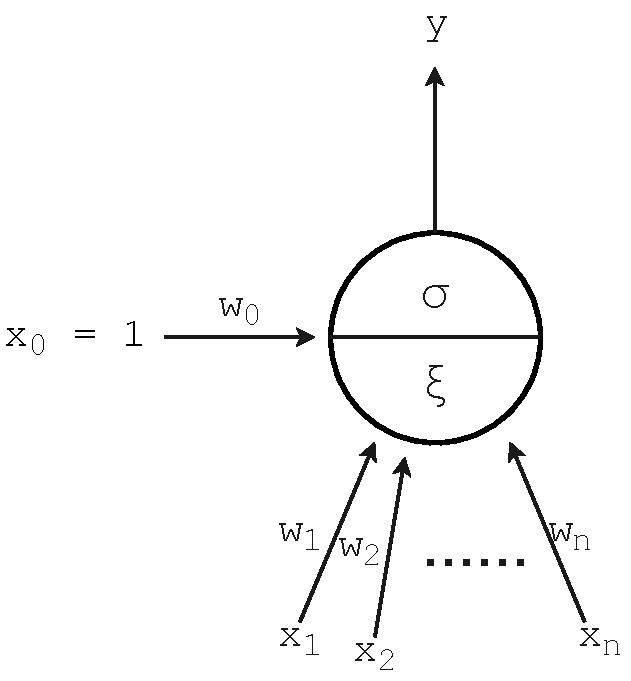
\includegraphics[width=\textwidth]{tex/images/perceptron}
  \caption{Artificial neuron}
\end{subfigure}%
\hfill
\begin{subfigure}{.55\textwidth}
  \centering
  \begin{itemize}

	\item $x_1, \cdots, x_n$ are real \textbf{inputs}
	\item $x_0$ is always equal to 1
	\item $w_0, w_1, \cdots, w_n$ are real \textbf{weights}
	\item $\xi$ is inner \textbf{potential}, \\$\xi = w_0 + \Sigma_{i=1}^n w_i x_i$
	\item $y$ is real \textbf{output} given as \\ $y = \sigma(\xi)$
	\item $\sigma$ is an \textbf{activation function}

	\end{itemize}
\end{subfigure}
\end{figure}

\section{Activation}

An activation function $\sigma: \mathbb{R} \rightarrow \mathbb{R}$ is applied to the inner potential $\xi$, and it defines the output value of perceptron. It introduces a powerful tool into machine learning, and that is \textbf{non-linearity}. Without the activation, the potential by itself is a simple polynomial of a degree of one. That would limit the learning ability of the neural network into being a simple regression model. However, using different activation functions, we can adapt the model to more complicated mappings.

\begin{figure}[h]

\centering
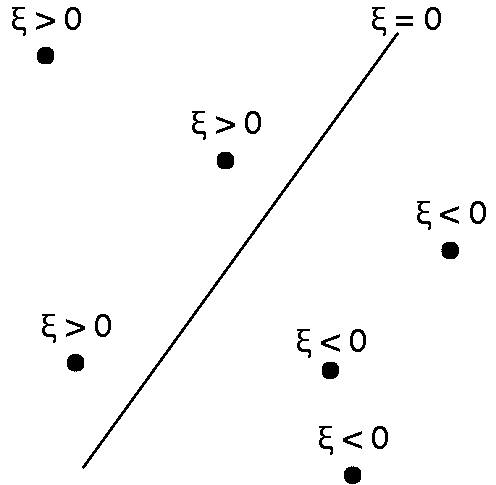
\includegraphics[width=0.45\textwidth]{tex/images/activation-vis}
\caption{Visualization of binary step activation function, which defines a separation hyperplane in n-dimensional space.}
\end{figure}

\noindent
Some desirable properties\cite{wiki:activation} of an activation function include:

\begin{itemize}

\item \textit{non-linearity} - in order to map more complex functions (allows universal function approximations)
\item \textit{continuous differentiability} - the necessity for gradient-based optimization methods
\item \textit{range} - for infinite range, training is generally more efficient
\item \textit{monotonicity} - the error surface associated with a single-layer model is guaranteed to be convex
\item \textit{approximates identity near the origin} - initial weights can be randomized with small differences around the origin

\end{itemize}

\noindent
Here are some examples of activation functions\cite{activation_list}:

\subsection*{Identity}

\begin{figure}[H]
\raggedright
\begin{subfigure}{.25\textwidth}
  \centering
  \[ f(x) = x \]
\end{subfigure}%
\begin{subfigure}{.25\textwidth}
  \centering
  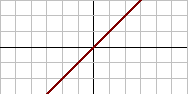
\includegraphics[width=\textwidth]{tex/images/activation/identity}
\end{subfigure}
\end{figure}

\noindent
Effectively remain the potential unchanged. 

\subsection*{Binary step}

\begin{figure}[H]
\raggedright
\begin{subfigure}{.35\textwidth}
  \centering
   \[
f(x) = \begin{cases}
       0 & x < 0 \\
       1 & x \geq 0 \\
     \end{cases} \]
\end{subfigure}%
\begin{subfigure}{.25\textwidth}
  \centering
  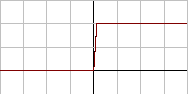
\includegraphics[width=\textwidth]{tex/images/activation/binstep}
\end{subfigure}
\end{figure}

\noindent
Basic activation function, transforms potential into a binary signal. However, this function is not differentiable.
      
\subsection*{Sigmoid}

\begin{figure}[H]
\raggedright
\begin{subfigure}{.28\textwidth}
  \centering
  \[ f(x) = \frac{1}{1 + e^{-x}} \]
\end{subfigure}%
\begin{subfigure}{.25\textwidth}
  \centering
  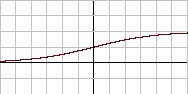
\includegraphics[width=\textwidth]{tex/images/activation/sigmoid}
\end{subfigure}
\end{figure}

\noindent
Smoothened binary step activation function, maps a real value potential into $(0,1)$ range. One of the most popular functions in the ANN's, mainly in the early era of machine learning. It introduces non-linearity. It suffers from vanishing gradient problem\footnote{described in subsection \ref{vanishing_gradient}} and have slow convergence. Furthermore, it is not zero centered, which make optimization harder.
 
\subsection*{TanH}

\begin{figure}[H]
\raggedright
\begin{subfigure}{.5\textwidth}
  \centering
  \[ f(x) = tanh(x) = \frac{(e^x - e^{-x})}{(e^x + e^{(-x)})} \]
\end{subfigure}%
\begin{subfigure}{.25\textwidth}
  \centering
  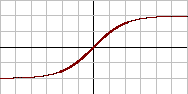
\includegraphics[width=\textwidth]{tex/images/activation/tanh}
\end{subfigure}
\end{figure}

\noindent
Unlike sigmoid, hyperbolic tangent is zero centered. It usually performs better than sigmoid. However, it stills suffers from vanishing gradient problem.

\subsection*{Rectified linear unit (ReLU)}

\begin{figure}[H]
\raggedright
\begin{subfigure}{.35\textwidth}
  \centering
   \[
f(x) = \begin{cases}
       0 & x < 0 \\
       x & x \geq 0 \\
     \end{cases} \]  
\end{subfigure}%
\begin{subfigure}{.25\textwidth}
  \centering
  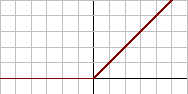
\includegraphics[width=\textwidth]{tex/images/activation/relu}
\end{subfigure}
\end{figure}

\noindent
One of the most popular function in recent years. As opposed to previous ones, it does not have an issue with vanishing gradient. It is simple and efficient. The limitation is that it should only be used within hidden layers of a model, often combined with softmax in the output layer. It turned out to be very useful in deep learning, where traditional activation functions struggle. For example in \cite{relu_faster}, the convolutional network was able to converge six times faster with ReLU, than with tanh.

\subsection*{Leaky ReLU}

\begin{figure}[H]
\raggedright
\begin{subfigure}{.38\textwidth}
  \centering
  \[
f(x) = \begin{cases}
       0.01x & x < 0 \\
       1 & x \geq 0 \\
     \end{cases} \]  
\end{subfigure}%
\begin{subfigure}{.25\textwidth}
  \centering
  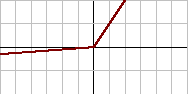
\includegraphics[width=\textwidth]{tex/images/activation/lrelu}
\end{subfigure}
\end{figure}

\noindent
One issue present in ReLU is that it allows the gradient to die off, which is not necessarily a bad thing, though it may result in dead neurons that will never activate on specific data points. To counter this, leaky ReLU's were introduced. To keep the updates alive, they add a small slope into their negative parts (usually with the factor of around 0.01).
   
\subsection*{Randomized ReLU}

\begin{figure}[H]
\raggedright
\begin{subfigure}{.35\textwidth}
  \centering
  \[
f(r, x) = \begin{cases}
       rx & x < 0 \\
       1 & x \geq 0 \\
     \end{cases} \] 
\end{subfigure}%
\begin{subfigure}{.25\textwidth}
  \centering
  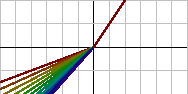
\includegraphics[width=\textwidth]{tex/images/activation/rlrelu}
\end{subfigure}
\end{figure}

\noindent
Another variant of ReLU randomizes the factor in leaky ReLU's.

\subsection*{Softmax}
\label{subsection:softmax}

\begin{figure}[H]
\raggedright
\begin{subfigure}{.25\textwidth}
  \centering
  \[ f(x_j) = \frac{e^{x_j}}{\sum_i e^{x_i}} \]
\end{subfigure}%
\begin{subfigure}{.25\textwidth}
  \centering
  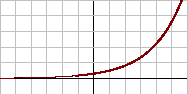
\includegraphics[width=\textwidth]{tex/images/activation/softmax}
\end{subfigure}
\end{figure}

\noindent
Softmax is usually used alongside the ReLU's in the output layer of a deep neural network. It has two nice properties:

\begin{itemize}

\item each value ranges in $[0, 1]$
\item the sum of all values is always 1

\end{itemize}

This is useful when modeling a particular probability distribution. It is used as the estimate of the class distribution for a given input.

\section{Artificial neural network}

Artificial neural network\cite{nn_book} or feed-forward neural network is a directed acyclic graph of artificial neurons organized into several layers, where the following holds:

\begin{itemize}

\item the first layer is called the \textit{input layer}, and the output of neurons is equal to the input vector $\overrightarrow{X}$

\item the last layer is called the \textit{output layer}, and it provides the output $\overrightarrow{Y}$

\item the other layers are called the \textit{hidden layers}

\item outputs of each neuron (except for the output layer) serve as inputs of neurons in the higher layer

\item every two neighboring layers $i$ and $i+1$ make a complete bipartite graph

\item no non-neighboring layers have a connection between them

\end{itemize}

\noindent
In the next sections, we are going to use the following terminology:

\begin{itemize}
  \item every neuron is represented as a distinct natural number (i.e neuron 1, 2, and so forth)
  \item $\xi_i$ is the inner potential of the neuron $i$
  \item $y_i$ is the output of the neuron $i$
  \item $w_{ji}$ is the weight from neuron $i$ to neuron $j$
  \item $j_{\leftarrow}$ is the set of all neurons $i$ such that there exist an edge $w_{ji}$
  \item $j_{\rightarrow}$ is the set of all neurons $i$ such that there exist an edge $w_{ij}$

\end{itemize}

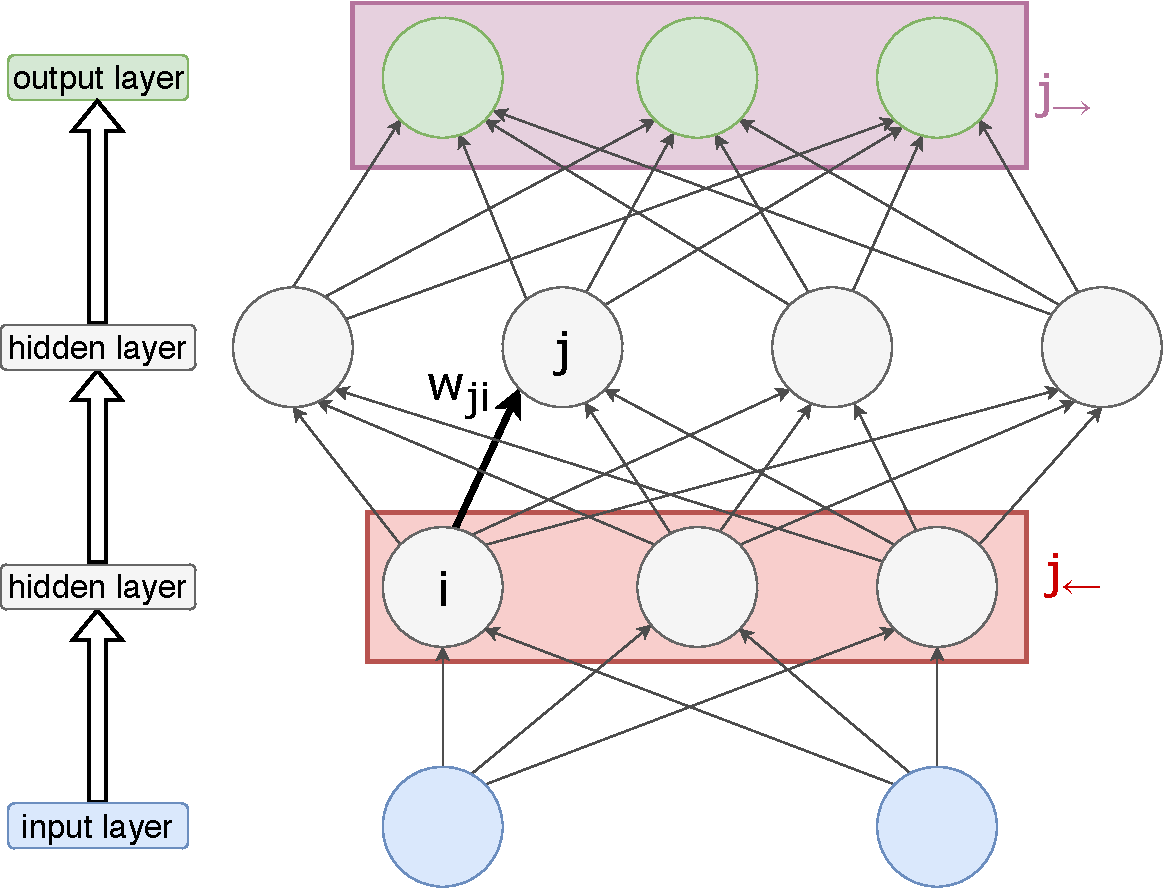
\includegraphics[width=0.8\textwidth]{tex/images/ann}

The neural network is continuously evolving, the states and connections of neurons are changing, weights are adapting. In term of these changes within a period, we can divide the network dynamics into three subcategories:

\begin{itemize}
  \item \textit{organizational} - change in topology
  \item \textit{active} - change in state
  \item \textit{adaptive} - change in configuration
\end{itemize}

\section{Active dynamics}

The values in the input layer are set to the input vector $\overrightarrow{X}$. The forward propagation algorithm is then applied. Starting from the lowest layer, each layer using the output from the previous one updates its neurons. Neuron $j$ updates its inner potential:

$$ \xi_j = w_0 + \sum_{i \in j_{\leftarrow}} w_{ji} y_i $$

The output of neuron $j$ is $y_j = \sigma_j (\xi_j)$. The exception is the input layer, where $y_j = \xi_j$.

\section{Adaptive dynamics}

\textit{Adaptive dynamics} specify the initial configuration of the network and the way, in which the configuration evolves during the training process. Initially are all weights set randomly. In order to update the network weights, we need to define the loss function.

\subsection{Loss function}

At its core, a loss function\cite{loss} is a simple method of evaluating how well the model adapts to the dataset. The higher the loss value is, the more inaccurate the model is. The main goal of the training process is to find the global minima of the loss function. Furthermore, the loss function is differentiable.

Given the set of training data $\tau = \lbrace (\overrightarrow{X_k}, d(\overrightarrow{X_k})) \vert k = 1, \cdots, p \rbrace$, where $\overrightarrow{X_k}$ is a feature, that is fed to the network and $d(\overrightarrow{X_k})$ is a label, that we would like to get as an output from the network.

The loss function is checking the difference between the network's output $\overrightarrow{Y}$ the actual label $d(\overrightarrow{X})$. From now on, we will refer to the output layer as OL in this section.

\subsection*{MSE}

One of the simplest loss function used in machine learning methods is \textit{Mean Squared Error} (of MSE for short):

$$ E(\overrightarrow{w}) = \sum_{k=1}^{p} E_k(\overrightarrow{w}) = \sum_{k=1}^{p} \frac{1}{2} \sum_{j \in \text{OL}} (y_j(\overrightarrow{w}, \overrightarrow{X_k}) - d(\overrightarrow{X_k})_j)^2 $$

\noindent
It is widely used in linear regression analysis.

\subsection*{Cross entropy}

Another very popular loss function, which we used is \textit{cross entropy loss}\cite{cross_entropy}. It is a straightforward modification of a basic likelihood function with logarithms over the probability $p$. It penalizes heavily for being very confident and very wrong. 

In order to transform the output vector $\overrightarrow{Y}$ into the probability distribution $P(\overrightarrow{Y})$ we usually use a softmax activation function in the output layer (as described in section \ref{subsection:softmax}). With the output transformed into a probability vector, we can use the cross entropy:

$$ E(\overrightarrow{w}) =  \sum_{k=1}^{p} E_k(\overrightarrow{w}) = \sum_{k=1}^{p} \sum_{j \in \text{OL}} - d(\overrightarrow{X_k})_j \ln{P(y_j(\overrightarrow{w}, \overrightarrow{X_k}))}$$

\subsection{Gradient descent and backpropagation}

Stochastic gradient descent\cite{deep_learning_SGD} and its variants are probably the most used optimization algorithms for machine learning in general. To update weights according to the given loss function, we need to compute the gradient at any given point on the function in the hyperplane. The gradient vector points towards the closest local minimum. It is the direction in which we want to update our weights.

The learning algorithm is computing the sequence of weight vectors $\overrightarrow{w}^{(0)}, \overrightarrow{w}^{(1)}, \overrightarrow{w}^{(2)}, \cdots$, where:

\begin{itemize}

\item $\overrightarrow{w}^{(0)}$ is the initial vector set randomly (usually weights close to 0)
\item in the $(i+1)$-th step is $\overrightarrow{w}^{(t+1)}$ computed as:

\begin{flalign}
\notag w_{ji} & = w_{ji}^{(t)} + \Delta w_{ji}^{(t)} & \\
\notag \Delta w_{ji}^{(t)} & = - \epsilon(t) \frac{\partial E}{\partial w_{ji}}(\overrightarrow{w}^{(t)}) & 
\end{flalign}

\item $\Delta w_{ji}^{(t)}$ is the weight difference in the step $(t+1)$ and $0 < \epsilon(t) < 1$ is the learning rate in the step $(t+1)$

\begin{flalign}
\notag \frac{\partial E}{\partial w_{ji}} & = \sum_{k=1}^p  \frac{\partial E_k}{\partial w_{ji}} & \\
\notag \frac{\partial E_k}{\partial w_{ji}} & = \frac{\partial E_k}{\partial y_j} \cdot \sigma_{j}^{'}(\xi_j) \cdot y_i & 
\end{flalign}

\begin{flalign}
\notag \frac{\partial E_k}{\partial y_j} &  = 
     \begin{cases}
       y_j - d(\overrightarrow{X_k})_j & \quad\text{for } j \in \text{ OL} \\
       \sum_{r \in j^{\rightarrow}} \frac{\partial E_k}{\partial y_r} \cdot \sigma_{r}^{'}(\xi_r) \cdot w_{rj} & \quad\text{otherwise} \\
     \end{cases} &
\end{flalign}

\end{itemize}

\noindent
While the feed-forward phase was evaluated from the input layer towards the output layer, the weight update is done in the different direction. Starting from the output layer, we are using the partial derivatives from the layer above to evaluate the current layer. This process is also known as \textit{backpropagation}.

There are two general types of weight update algorithms:

\subsection*{Batch algorithm}

It is the approach described above. It takes a batch of data points in each and computes only one weight update for all of these points together. The advantages include:

\begin{itemize}

\item the direction of the descent is identical to the gradient descent vector
\item parallelism is easy to implement - data point losses can be computed secludedly

\end{itemize}

\noindent
The problems of a batch algorithm:

\begin{itemize}

\item memory consumption
\item redundant data do not add any information to the gradient
\item is more likely to end up in some local minimum than the online algorithm

\end{itemize}

\subsection*{Online (stochastic) algorithm}

An online algorithm is essentially a batch algorithm, where batch consists of only one data point\footnote{point can be taken deterministically or at random (thus stochastic)}. Instead of the whole batch, we update the weight for each data point:

$$ \Delta w_{ji}^{(t)} = - \epsilon(t) \frac{\partial E_k}{\partial w_{ji}}(\overrightarrow{w}^{(t)}) $$

\noindent
Therefore it is not taking the path of gradient descent exactly, but rather "zigzag" alongside the gradient descent vector. The advantages include:

\begin{itemize}

\item it has a better chance of escaping the local minimum than batch algorithm
\item less memory consumption
\item faster (especially on redundant data)

\end{itemize}

\noindent
The problems of an online algorithm:

\begin{itemize}

\item not suitable for parallelism
\item can behave weirdly, because it is not taking the direct path to minimum

\end{itemize}

\section{Issues}

There are widely known issues when working with neural networks, which have to be taken into consideration when working with models. In this section, we will mention just a couple, which we encountered and had to deal with.

\subsection{Dataset split}

Very simple, but very crucial mechanism used in machine learning is to define three separate sets (\textit{train}, \textit{valid} and \textit{test}). These sets have to be disjoint. It is necessary to use \textit{valid} set during the training process and different \textit{test} set for model evaluation, once the model is trained. The reason behind is that always the model will have a slight bias towards the \textit{valid} test compared to the independent \textit{test} set.

\subsection{Vanishing gradient problem}

\label{vanishing_gradient}

The \textit{vanishing gradient problem}\cite{vanishing_gradient} is a difficulty found in training ANN's. The problem is, that in some cases the gradient will be vanishingly small with the impact on weight update. It gets more apparent with many-layered feedforward networks as well as with recurrent networks. Activation functions such as \textit{hyperbolic tangent} and \textit{sigmoid} suffer from vanishing gradient, while others like ReLU or Leaky ReLU do not.

\section{Model evaluation}
\label{nn-metrics}

After the training process, a huge emphasis is put into the model evaluation. With the incorrect evaluation methods, even the poorly trained model can have a good overall score. Several factors have to be taken into consideration like the uneven distribution of data classes, false negatives, and false positives or the classification interchanging between two groups.

\subsection{Confusion matrix}

In the field of machine learning and specifically the problem of statistical classification, a \textit{confusion matrix}\cite{conf_matrix} is a two-dimensional matrix $n \times n$, where $n$ is the number of classes. Each row of the matrix represents the instances in a predicted class while each column represents the instances in an actual class. It is the most verbose output of the evaluation. We can see the wrongly classified classes, but also the classes which the model misclassified into. 

\begin{figure}[h]
\centering
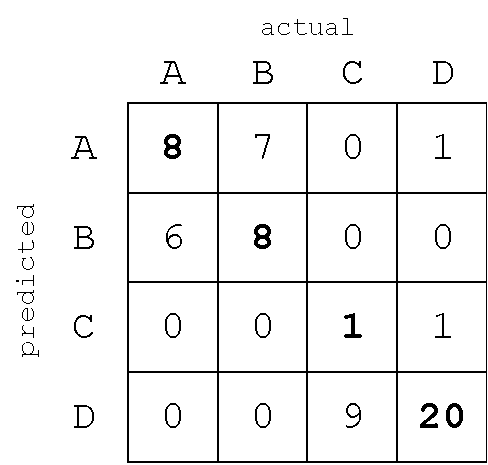
\includegraphics[width=0.37\textwidth]{tex/images/conf_matrix}
\caption{Example of a classification matrix.}
\label{conf_matrix}
\end{figure}

\noindent
In Figure \ref{conf_matrix}, we can see the classification matrix for four classes. The correctly classified cases lie on the main diagonal. Several observations about our model can be seen. First of all, our model almost always misclassifies class \textit{C} as class \textit{D}. Furthermore, the model has difficulties distinguishing between classes \textit{A} and \textit{B} (it would be a good idea to merge these classes).

\subsection{Metrics}

There are four standard metrics \cite{nn-metrics} for model evaluation: \textbf{accuracy}, \textbf{precision}, \textbf{recall}, and \textbf{f1}. Apart from the standard metrics accuracy, the other metrics represent the cost of having false positives and false negatives. Let us take a simple binary confusion matrix:

\begin{table}[h]
\centering
\begin{tabular}{|r|c c|}

\hline 
& $A$ & $\neg A$ \\
\hline 
$A$ & TP & FP \\
$\neg A$ & FN & TN\footnotemark\\

\hline

\end{tabular}

\end{table}

\footnotetext{true positive / false positive / false negative / true negative}

\noindent
We define the four metrics as followed:

\begin{align*}
\textit{accuracy } & = \frac{TP + TN}{TP + FP + FN + TN} & \\
\textit{precision } & = \frac{TP}{TP + FP} & \\
\textit{recall } & = \frac{TP}{TP + FN} & \\
\textit{F1 } & = \frac{2 \times \textit{ precision } \times \textit{ recall}}{\textit{precision } + \textit{ recall}} &
\end{align*}

\begin{itemize}

\item \textbf{accuraccy} - is the standard metric for classifiers, we take the ratio of correctly classified data to the whole dataset. The problem with accuracy is, that it suffers from unbalanced datasets, where the bigger groups can artificially increase accuracy.

\item \textbf{precision} - talks about how precise the model is out of positive predictions and how many are actual positives. It is useful to use when the cost of false positive is high.

\item \textbf{recall} - works the other way around, where we calculate how many of positives are really true positives and not just false negatives. It is useful to use when the cost of false negative is high.

\item \textbf{f1 score} - is a balance between precision and recall and serves as an alternative to the accuracy

\end{itemize}

\section{Grid search}
\label{section-grid-search}

In this thesis, we used the method called \textbf{grid search}\cite{grid-search}. When there are a couple of hyperparameters, the common practice
is to perform a grid search. For each hyperparameter, the user selects a
small finite set of possible values to explore. The grid search algorithm
then trains models for every joint specification of hyperparameter
values in the Cartesian product of the set of values for individual
hyperparameters. The experiment then yields the best model and hyperparameter choice. 





  \chapter{Dataset}
\label{chapter-dataset}

For this thesis, we were provided with the dataset consisting of more than 30 sources collected from different software libraries, hardware authentication devices (or cards) and HSM's\footnote{Hardware security modules}. 
Some of the software libraries had the option of so-called FIPS module, which is a security standard, that put some requirements on generated primes and their distribution, namely available in \textit{PGP SDK 4}, \textit{Libgcrypt} and \textit{OpenSSL}. Furthermore, every source had one or more development versions. 

Considering both of these options, we split our dataset into 64 distinct sources based on their version and whether or not they had the FIPS module activated when generating primes. Every source was represented by a couple of CSV files, with fields $n, e, d, p, q$ and $t$ (time of generation). Three key lengths were present (512b, 1024b and 2048b), with most of the data originated from 512b or 1024b.

All in all, a total of more than 146 million keys were collected with roughly 75.5 million of 512b and 65.4 million of 1024b keys. These two datasets were used for machine learning and preparing classification models. A complete overview of the dataset can be seen in Appendix \ref{appendix-dataset}.

In the article by CROCS lab\cite{svenda_1}, different sources were merged into 13 disjoint groups using clustering on the mask of 9 selected bits. Using the naive Bayes classifier, they were able to classify a random sample of keys with the accuracy of 40.34 \%. Therefore, in this thesis, we tried to pick up on these results and further extend the accuracy by using other classifiers while focusing specifically on neural networks.

\section{Dataset analysis}

\label{chapter-analysis}

Before attempting to create a working classifier, the analysis of the dataset and subsequent feature engineering was necessary. We scanned the whole dataset, extracting features from public product $n$. We focused mainly on the bit value on every position and the remainder when divided by a specific number. With every feature, we counted the relative frequency of every possible value. Because of the huge number of keys, we needed to run this analysis distributively on Metacentrum\footnote{distributed cloud computing over CESTNET}.

\subsection{Modular analysis}

As in the full CROCS report\cite{svenda_full}, we did a similar analysis on the full dataset. With every key, we computed a modulo over first 30 natural numbers, starting with 3, while focusing mainly on prime numbers. We were looking for any irregularities in distribution of the remainders. Specifically, with prime numbers $p$, the remainder should be uniformly distributed between 1 and $p-1$. Several sources showed bias, namely:

\begin{itemize}

\item \textit{mod 3} - sources 2,3 (G\&D SmartCafe 4.x and 6.0), 11-14 (OpenSSL without FIPS module) and 19, 20, 21 (NXP J2D081, NXP J2E145G, YubiKey NEO) were always giving a remainder of 1.

\item \textit{mod 4} - sources 1, 2, 3 (G\&D SmartCafe) 4 (GNU Crypto 2.0.1) 6, 7, 8, 9 (NXP J2A*, NXPJ3A*, NXP JCOP 41 V2.2.1), 10 (Oberthur Cosmo Dual 72K) and 19, 20, 21 were always giving a remainder of 1. Sources that were giving a remainder of 1 modulo 3 and 4 are using Blum integers.

\item \textit{module 11} - sources 16, 17, 18 (Infineon, Yubikey and Yubikey Nano) were giving only remainders of 1 or 10. Sources 11, 12, 13, 14, 19, 20 had slight bias towards the remainder of 1.

\end{itemize}

\noindent
Full results of modular analysis can be seen in Appendix \ref{appendix-modular-analysis}.

\subsection{Bit analysis}

Another analysis focused on full bit analysis. Similarly, as in the previous one, we computed the relative frequency (or probability of 0) on every bit position with each source. This kind of analysis took a more significant amount of time and needed to be computed distributively. It took a couple of hours compared to the estimated time of up to one week when computing on the local machine. The analysis showed a significant bias in the first 6 most significant bits, mostly:

\begin{itemize}

\item \textbf{1st MSB} was always 1 (for bit length padding) with one exception of source 15 (PGP SDK FIPS 4), which contained a majority of its keys with shorter bit length.

\item \textbf{2nd - 4th MSB} could distinguish a lot of groups (i.e. 16-18 or 1-3), because of wider probability distribution.

\item \textbf{5th - 6th MSB} still had slight bias in probability distribution for some groups (4, 19-21, 31-40)

\item \textbf{2nd LSB} could distinguish mostly groups that were using Blum primes (1-4, 6-10, 19-21)

\end{itemize}

\noindent
Full results of bit analysis can be seen in Appendix \ref{appendix-bit-analysis}.

\subsection{Feature engineering}

\label{feature-engineering}

Based on the previous analysis we extracted the following features from the public key to feed to the network:

\begin{itemize}

\item all moduli remainders up to 30 represented as binary vector\footnote{For example for $x \equiv 1 \pmod{5}$, the feature vector is $(1,0,0,0)$, $x \equiv 2 \pmod{5}$ - $(0,1,0,0)$, $\cdots$}

\item The key itself

\end{itemize}

\noindent
The performance of the network was similar regardless of using the full key, or just the biased bits.

\subsection{Source grouping}
If we look closely on the full analysis in Appendix \ref{appendix-analysis}, we can see that based on the feature engineering we can natively group sources, that share the distribution. We obtain 13 groups\footnote{Same grouping was obtained by cluster analysis in \cite{svenda_1}}:

\vspace{5mm}

\noindent
\begin{tabular}{|r|l||r|l||r|l|}

\hline

\textbf{G1} & 1 & \textbf{G6} & 10 & \textbf{G10} & 19, 20, 21 \\
\textbf{G2} & 2, 3 & \textbf{G7} & 11, 12, 13, 14 & \textbf{G11} & 22 - 29 \\
\textbf{G3} & 4 & \textbf{G8} & 15 & \textbf{G12} & 30 - 40 \\
\textbf{G4} & 5 & \textbf{G9} & 16, 17, 18 & \textbf{G13} & 41 - 64 \\
\textbf{G5} & 6, 7, 8, 9 & & & & \\

\hline

\end{tabular}

  \chapter{Implementation}
\label{chapter-implementation}

As a part of this thesis, we designed a simple tool able to work with our dataset and execute various tasks over it. The main idea was to unify the interface for models, so many different models can be run just via command line. This proved to be essential when running many models concurrently on Metacentrum or in the local machine. The whole tool is written in Python 3.6, and it is accessible via one common command-line interface.

\section{Used technologies}

\subsection{Pandas}

To work with CSV files of a length of more than 30 million lines, one does need to use the appropriate framework for it. We chose the pandas \cite{pandas} library. Actively supported today by a community, it is a BSD-licensed library providing high-performance, low-level optimized and easy-to-use data structures for data analysis for \textit{Python} programming language. Pandas stores its data in so-called dataframes \cite{pandas-df}, which are working on the same principle as in the \textit{R} language. They can store two-dimensional size-mutable heterogeneous tabular data and allow arithmetic operations to align on both row and column. Furthermore, pandas can work with huge CSV files using python generators. We used it to read/write CSV files and transform dataframes to fit the neural networks. 

\subsection{TensorFlow}

TensorFlow \cite{tensorflow} is an open source software library for high-performance numerical computation. Tensorflow was developed by the Google Brain team for internal Google use. It was released under the Apache 2.0 open source license on November 9, 2015. Its flexible architecture allows easy deployment of computation across a variety of platforms (CPUs, GPUs, TPUs), and from desktops to clusters of servers to mobile and edge devices. Originally developed by researchers and engineers from the Google Brain team within Google’s AI organization, it comes with strong support for machine learning and deep learning, and the flexible numerical computation core is used across many other scientific domains. Its core is written in C++ and CUDA, thus it is highly optimized for parallel computations on GPU.

\subsection{Keras}

Keras \cite{keras} is arguably one of the most popular python tensorflow frontends for a quick and simple definition of networks. In comparison to tensorflow, Keras is very layer-oriented and has an intuitive user-friendly API. All models, that we trained were defined over Keras framework. The simplicity of Keras framework can be shown in an example of a concrete model, that we used. The whole model is defined in just 5 lines of code:

\begin{minted}[ framesep=2mm,
                autogobble,
                frame=lines]{python}
import keras
inputs = keras.layers.Input(shape=(input_dimension,))
x = keras.layers.Dense(1024, activation='relu')(inputs)
outputs = keras.layers.Dense(output_dimension, 
                             activation='softmax')(x)
model = keras.models.Model(inputs=inputs, outputs=outputs)
model.compile(loss=keras.losses.categorical_crossentropy,
              optimizer=keras.optimizers.Adadelta(),
              metrics=['acc'])

\end{minted}

\subsection{Scikit-learn}
 
For comparison to traditional models, we chose the sklearn \cite{scikit} package, the native package for basic machine learning and evaluation. We used classifiers such as KNN, Naive Bayes, decision trees or support vector classifiers\footnote{List of all possible classifiers can be found in \url{http://scikit-learn.org/stable/supervised\_learning.html\#supervised-learning}}.  

\subsection{Docker}

\label{docker}

Initially, the tool was developed on the local Linux machine, because it was dependent on third-party Unix binaries, as well as it was later deployed to Metacentrum cloud, which is Unix native. However, we needed to develop and run it also on other architectures. One approach is to install virtual machines on the desired host, setup Unix environment and then run the tool. The better, more lightweight approach would be to use containers, namely Docker \cite{docker}.

Docker encapsulates the application, running environment, dependencies and architecture into a self-contained unit that can run anywhere. It is a more lightweight virtual machine because containers in comparison to virtual machines share the host system’s kernel with other containers \cite{docker-blog}. By defining dockerfile, we provided any user the option to run this tool on its own local machine.

\subsection{Python generators}

\label{python-generators}

During the training process, we were working with huge files with over several millions lines. Even as raw strings, that could take up to 2 GB of memory. Furthermore, we transformed the keys into numpy arrays, which was infeasible memory-wise as it could easily take more than 20-25 GB of RAM. Rather than allocating such memory in Metacentrum, one can provide a better solution - python generators \cite{python-gen}. 

Generator functions allow you to declare a function that behaves like an iterator, i.e. it can be used in a loop. The main advantage is that the data is fetched during the runtime as the iteration of the for loop is always called on demand.

\begin{minted}[ framesep=2mm,
                autogobble,
                frame=lines]{python}
def get_data():
    n = 1
    while True:
        yield n
        n += 1
		
for n in generate_numbers():
    ...
\end{minted}

This simple example shows how to generate natural numbers. Instead of natural numbers we simply take a chunk of lines from the source CSV file resulting in saving the memory consumption. Therefore we can run huge datasets also in local machine as well as take smaller resources on Metacentrum, thus increasing our chance of running our job in the queue.

\subsection{Click}

As our tool provides only command line interface, we chose the Click package \cite{click}, a command line interface creation kit. It provides decorator options for defining arguments and options with validation and automatic help generation. As a framework, it suited the necessary needs for the application and sped up the development process.

\section{Tasks}

During the implementation process, several distinct tasks were implemented in order to work with the original dataset, prepare the data for models to train and then classify. \autoref{figure-model} shows the flow of the application and its data. We named these tasks \textbf{SCAN, ANALYZE, GENERATE, TRAIN} and \textbf{CLASSIFY}.

We obtained a dataset in the form of around 2000 CSV files. First of all, we wanted to automate extracting the keys from distinct files and assigning class labels to it. Therefore, the \textbf{SCAN} task was implemented. We used it mainly to transform given dataset, which was badly structured without naming convention and difficult to extract keys from into more compact one. The transformed dataset could be used more efficiently for analysis and generating new datasets.

The newly generated compact dataset was then subjected to full analysis of features. For this purpose, the \textbf{ANALYZE} task was implemented. We used it to count the relative frequency of features that we presented in \autoref{chapter-analysis}.

Another task \textbf{GENERATE} was used to prepare custom generated datasets for machine learning models. Its main purpose was to be able to generate datasets with different class labels, replicate keys in training dataset, skip groups, skip files, merge several groups into one and others. We used this task throughout the whole training process to create datasets for models and tune them if the model was struggling in training.

The main task \textbf{TRAIN} was applied to the custom generated datasets. Its purpose was to feed data into the model, monitor performance and report the results of the training. Models are sharing the same interface. This allows to implement new model relatively simply and use the whole task for any model.

Models that are performing well can be used, evaluated and tested via \textbf{CLASSIFY} task using the same shared core with \textbf{TRAIN}.

\begin{figure}[H]
\centering
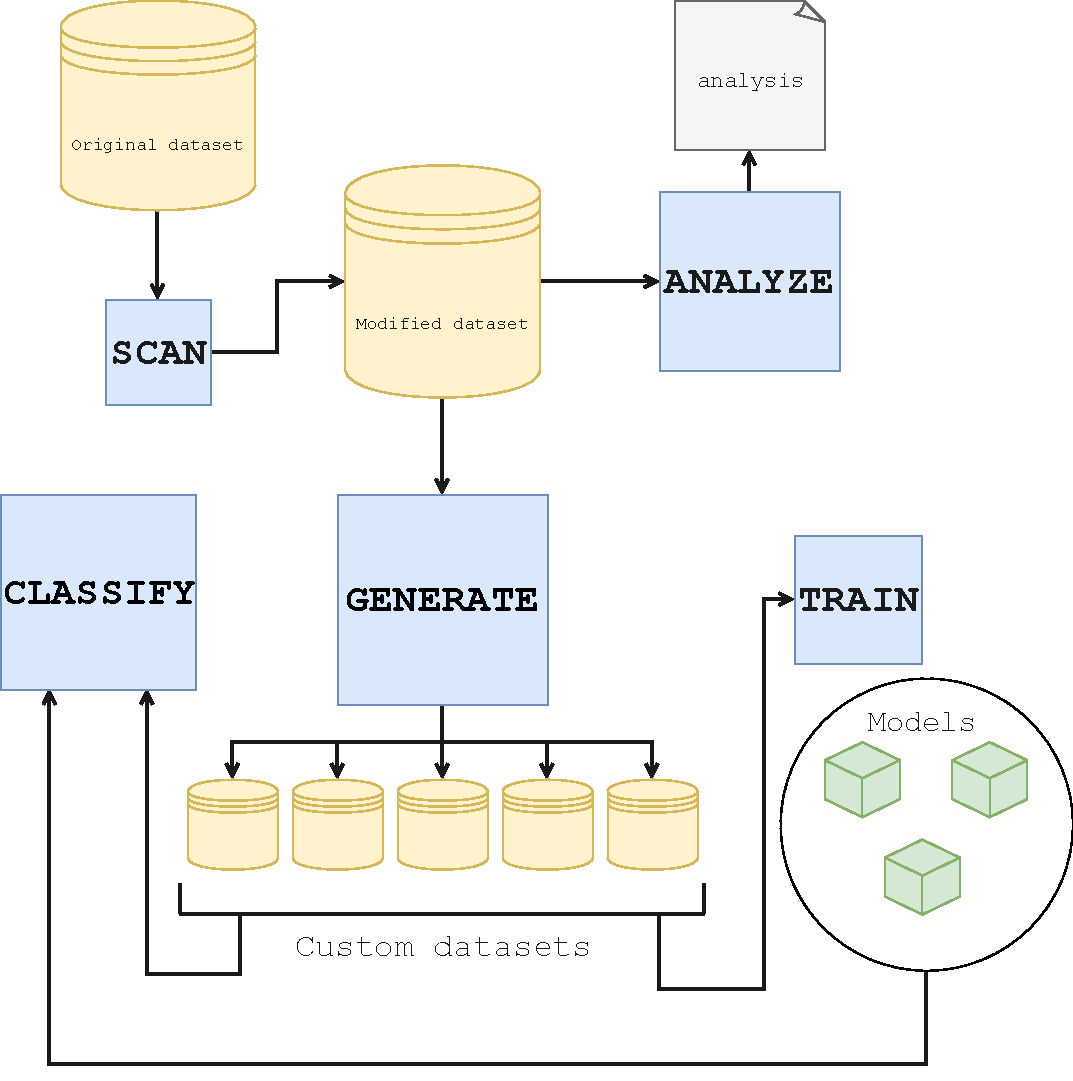
\includegraphics[width=0.65\textwidth]{tex/images/thesis_model}
\caption{Diagram of the application flow shows 5 distinct tasks (SCAN, ANALYZE, GENERATE, TRAIN, CLASSIFY) that we used to work with our dataset and perform machine learning on it.}
\label{figure-model}
\end{figure}

\subsection{SCAN task}

The original dataset was in the form of a directory hierarchy, where there was no specific namespace for different key length and sources. We needed a task to be able to create groups of sources, that would be corresponding to the same label. Then using this grouping generate a new dataset, which is well structured and easier to analyze.

The \textit{SCAN} task is using simple string matching with required (positive) keywords and forbidden (negative) keywords. Then it iteratively loops through all CSV files in given root directory and looks for file names that contain any positive keyword and not containing any negative keyword. Keywords are passed to the task via JSON structure. Here is an example of a JSON filter we defined over the original dataset, which scans all sources from group 13 with bitlength of 1024: 

\begin{minted}[ framesep=2mm,
                autogobble,
                frame=lines]{json}
{
    ...
    "13": {
        "required": [
            "Botan_1-5-6",
            "Botan_1-11-29",
            ...
            "WolfSSL_3-9-0",
            "WolfSSL_3-10-2"
        ],
        "forbidden": [
            "PGP_SDK_4_FIPS",
            "Libgcrypt_1-7-6_FIPS",
            "512",
            "2048"
        ]
    }
}

\end{minted}

\noindent
As a result, we obtain a JSON file, which contains groups of sources with a given label and a list of individual sources with the number of keys in them. This JSON file is used further by the \textit{GENERATE} task. Below we show the example of a generated JSON file from the previous filter:

\begin{minted}[ framesep=2mm,
                autogobble,
                frame=lines]{json}
{
    ...
     "13": {
            "group_name": "13",
            "keys_total": 31911043,
            "sources": [
                {
                    "length": 50001,
                    "name": "Feitian JavaCOS A22",
                    "path": "/Card/Feitian JavaCOS A22 1024b/1.csv",
                    "read_lines": 0
                },
                ...
            ]
     }
}

\end{minted}

\noindent
The use of \textit{SCAN} is shown in \autoref{appendix-scan}.

\subsection{ANALYZE task}

The problem with working with huge CSV files is memory consumption, as we usually are not able to load all lines into RAM at once. Fortunately, pandas library offers reading and processing such files in chunks of lines. 

When analyzing a huge file, we iterate it in chunks, extracting values for features from every key and then just incrementing the corresponding counter. In the end, we print the analysis to the user.

\begin{figure}[h]

\centering
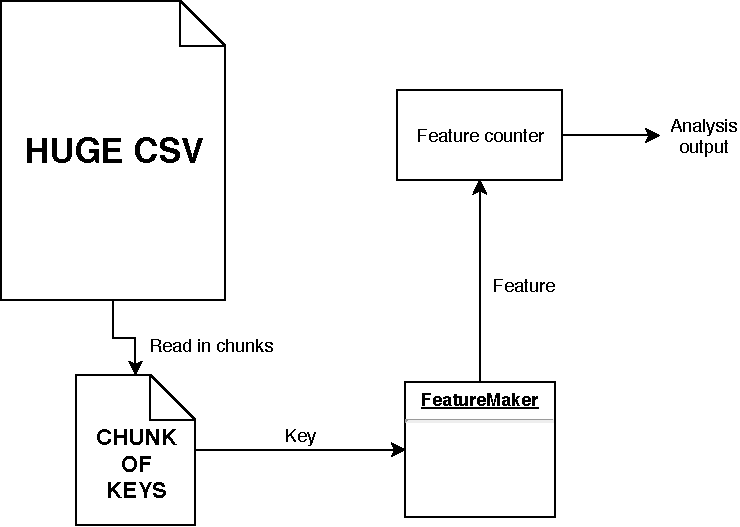
\includegraphics[width=0.5\textwidth]{tex/images/analyze_task}
\caption{\textit{ANALYZE} task flow.}

\end{figure}

Using \textit{SCAN} and \textit{GENERATE} we transformed the dataset to fit our purposes. We extracted all keys from each of available 64 sources of different key lengths and merged them all into single CSV files\footnote{i.e. for source 01 with we obtained 3 files, each with 512/1024/2048 keys respectively}. 

Having the dataset decoupled into several smaller CSV files, we could actually perform an analysis on each of these files distributively in the CESNET\footnote{Czech Educational and Scientific NETwork. See \url{https://www.cesnet.cz/?lang=eng}} cloud.

\subsection*{Feature Maker}

\label{feature-maker}

When analyzing the dataset, we obtained features to use in machine learning. Having them hardcoded would not be the best approach, as new features may occur or some features may not be used for some specific model. 

That is why we designed the Feature Maker. It is essentially a class, that is dedicated to the transformation of a raw key into the feature vector. Features may be added during runtime dynamically, usually via a configuration file. It gives us freedom of choosing a different set of features with every model (or during the analysis as well). Also, adding new feature does not change any other code, but the Feature Maker class itself to support our primary idea of extensibility and code decoupling. The features implemented so far:

\begin{itemize}

\item \textit{modulo} - can return either binary vector class (useful for machine learning) or remainder as a decimal number (useful for analysis)
\item \textit{bit} - returns specific bit (useful for mask in machine learning and analysis)
\item \textit{line} - returns whole line (shortcut of taking every bit)
\item \textit{xor} - return xor of two specified bits

\end{itemize}

\noindent
Feature Maker class uses couple lines of code. In the following simplified example, we define the feature maker, assign three features to it (modulo 3, modulo 7 and 38th LSB), then call the \texttt{get\_features\_from\_keys} which extract features for us. Adding or removing features can be performed between the 2nd and 4th line of code:

\begin{minted}[ framesep=2mm,
                autogobble,
                frame=lines]{python}

fm = FeatureMaker()
fm.add('mod3')
fm.add('mod', {'n': 7})
fm.add('bit', {'i': 37})
features = fm.get_features_from_keys(keys)

\end{minted}

\noindent
The user's settings and examples for \textit{ANALYZE} task are shown in \autoref{appendix-analyze}.

\subsection{GENERATE task}

One of the most important tasks we had to implement was the \textit{GENERATE} task. Given our modified dataset, we needed to generate smaller samples on which we could train different models. The whole process is managed by a Generator object, which reads the data specified by sources in a JSON file returned from the \textit{SCAN} task. It is responsible for preparing the datasets for tasks \textit{TRAIN}, \textit{ANALYZE} and \textit{CLASSIFY}. The Generator provides functionality to:

\begin{itemize}

\item generate single large CSV file (useful for \textit{ANALYZE}, \textit{CLASSIFY} and non-incremental models in \textit{TRAIN})
\item generate triplet of CSV files (train / test / valid) with ratio provided by the user (useful for incremental models in \textit{TRAIN})
\item shuffle target CSV file (may be disabled for \textit{ANALYZE} task)
\item relabel individual groups and merge several groups together to decrease the number of labels used
\item skip any source or the whole group of sources
\item take an arbitrary number of keys per group
\item take an arbitrary number of keys per line (meaning taking several keys as one line in the target CSV file), this reflects to the model having more keys from the same group in one training step
\item multiply keys in training data (useful for sampling, when a group has a limited amount of keys), this proved to be essential to create uniform training datasets

\end{itemize}

\noindent
The advantage of such an approach is that using the same original dataset, the user can generate a number of different datasets with his custom labels just by changing the configuration. Given the user's settings, the Generator works in several steps:

\begin{enumerate}

\item prepare the temporary CSV file that will store the new lines

\item prepare new labels mapping (user can merge different sources together, some labels might be unused)

\item iterate through sources specified in JSON

\item skip sources or groups that user specified

\item prepare a random sample of lines that will be read from the source, then read these lines in batches

\item prepare the line for the big CSV file (user can take more keys as one line in the final CSV)

\item multiply training sample by the ratio specified by the user

\item append line to the temporary file

\item shuffle temporary file and return as a new file (the final dataset)

\end{enumerate}

\noindent
All user's settings are specified in \autoref{appendix-generate}.

\subsection{TRAIN task}

The main task defined was task \textit{TRAIN}. As we provided all the tasks to prepare our datasets, we needed to implement the process of training the classifiers. The main idea was to split the process into two main logical units. The responsibility of the first one is to load the data a pass them on to the models. The second unit is the models themselves.

\subsection*{Loader}

The \texttt{Loader} interface is a part of the core of the application. It provides two main functions to feed data to the models:

\begin{itemize}

\item \texttt{get\_data()} - loads the whole file into memory and returns the numpy arrays, that can be fetched into the model (was necessary when working with models from scikit learn, that could not work with python generators). This is not suitable for larger files as they often don't fit into memory at once.

\item \texttt{get\_data\_generator()} - as mentioned in \autoref{python-generators}, when working with large files, it is more desirable to read them in chunks. Keras models do support training using python generators if we do provide one.

Reading the CSV in chunks using pandas, we extracted the features in every generator iteration and then yielded the data for the neural networks.

\end{itemize}

\noindent
As we were using two types of classifiers (from \textit{sklearn} and \textit{keras} libraries) and two types of datasets from \textit{GENERATE} task (either one big CSV file, or the CSV triplet), we provided two classes, that implemented this common interface:

\begin{itemize}

\item \texttt{LoaderSingle} - receive only one CSV file, and the split set ratios of the dataset. It computes the random permutation on lines, which are then distributed into their train / valid / test sets respectively. It directly corresponds to the single CSV files generated from the \textit{GENERATE} task, and it was implemented as the first simpler option.

\item \texttt{LoaderDataset} - the later implementation, receives the CSV triplet (train / test / valid) and does not need to compute the random permutation (which is memory consuming by itself). It directly corresponds to the CSV triplet from the \textit{GENERATE} task.

\end{itemize}

\noindent
The feature extraction from individual keys was done by \texttt{FeatureMaker} class with features specified by the user. More details were mentioned in \autoref{feature-maker}.

\subsection*{Models}

When designing the models, the main focus was put on extensibility. We implemented a common \texttt{Model} as a plain abstract class using the python \textit{abc}\footnote{see \url{https://docs.python.org/3/library/abc.html}} module. This allowed us to implement many models while keeping the same interface. Furthermore, as it is expected, that this application will be used later in the research, it is simple to add any other model just by implementing this interface and its methods:

\begin{itemize}

\item \texttt{fit()} and \texttt{fit\_generator()} - the model is given training and validation data in the form of either numpy arrays (\texttt{fit}) or an iterator (\texttt{fit\_generator}). The model trains itself.

\item \texttt{predict()} - given the input numpy vector, the model returns the prediction

\item \texttt{score()} - given the test data, the model returns an evaluation of itself

\item \texttt{get\_model\_info()} - return description as a string (used for logging the output)

\item \texttt{save()} - save model to given directory path

\item \texttt{load()} - load model from given directory path

\end{itemize} 

We implemented traditional classifiers from \texttt{scikit} library and multilayer perceptrons from \texttt{keras} library. For both of them, we implemented interfaces, that were direct children of the common \texttt{Model} interface. They implemented all the necessary interface methods to adapt them to used libraries. All the used models then inherited from their interface. The hierarchy can be seen in \autoref{model-inheritance}.

\begin{figure}[H]

\centering
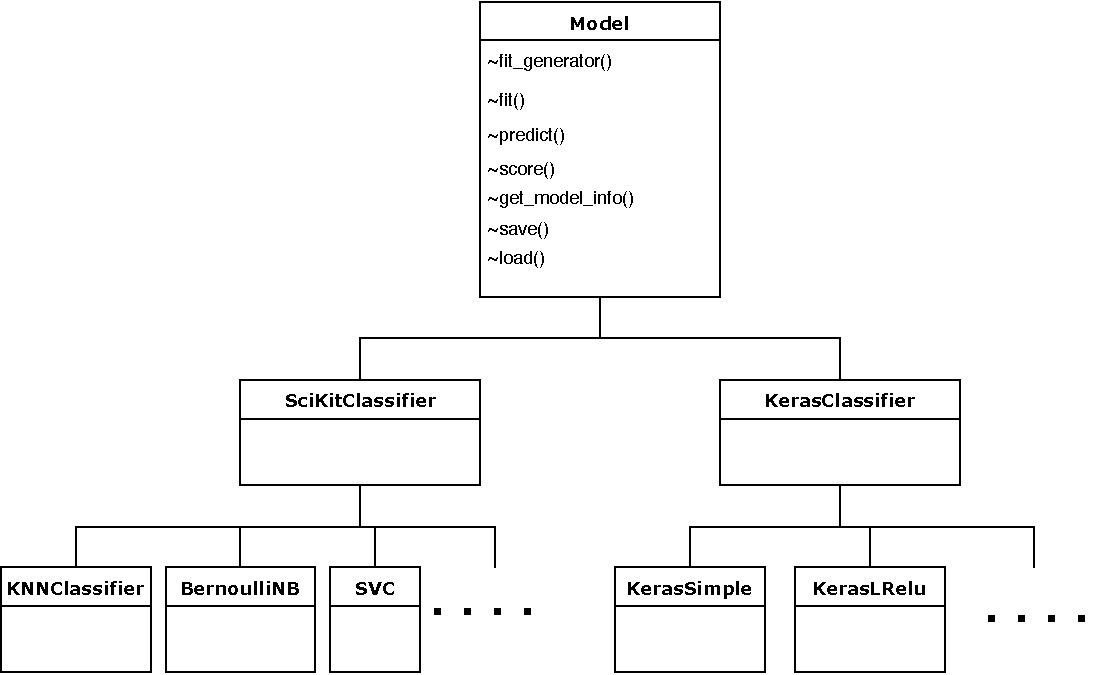
\includegraphics[width=0.75\textwidth]{tex/images/model_inheritance}
\caption{The hierarchy of implementation of the common \texttt{Model} interface. The second level groups the common logic for given library, the bottom level are individual implementations.}
\label{model-inheritance}

\end{figure}

From \texttt{scikit} we implemented most of the models listed in the documentation\footnote{\url{http://scikit-learn.org/stable/supervised\_learning.html\#supervised-learning}} (i. e. \texttt{KNN, NB, DecisionTree, SVC} and others). From \texttt{keras}, we implemented different multilayer perceptrons with topology specified by the user. Topology specifies hidden layers with their activation and the number of neurons, loss function, metrics, optimizer and activation of the output layer as JSON (example below).

\label{models-json}
\begin{minted}[ framesep=2mm,
                autogobble,
                frame=lines]{json}

 "Keras10": {"base": "KerasSimpleClassifier",
             "name": "Keras Multilayer Perceptron",
             "topology": {"hidden_layers": [{"activation": "relu",
                                             "number_of_neurons": 4096}],
                          "loss": "categorical_crossentropy",
                          "metrics": ["acc"],
                          "optimizer": "Adadelta",
             "output_layer": {"activation": "softmax"}}},

\end{minted}

\noindent
The models are trained in epochs, and after the training ends, they are evaluated with metrics defined in \autoref{nn-metrics}. For documentation and examples for \textit{TRAIN} tasks see \autoref{appendix-train}.

\subsection{CLASSIFY task}

The last (and for the end user, the most important one) is the \textit{CLASSIFY} task. The user compares trained models to the target CSV file and can either evaluate the model based on the labels given in the CSV file (similarly as in \textit{TRAIN} task) or can generate new labels for his dataset (useful for tagging unknown data). For documentation with examples see \autoref{appendix-classify}.

\section{Command line interface}
\label{cli}

We designed a simple CLI application using click library. The user can configure the application via the arguments or YAML configuration file (by default \textit{settings.yml}). Command line arguments have priority over YAML settings. For every task, the user can print help with the description of the task, an example of usage, arguments and yaml settings. The complete documentation with examples can be found in \autoref{appendix-running}.

\section{Multi platform development}

As we are using the third party binary, that is necessary for shuffling the datasets in the \textit{GENERATE} task, the application needs to run in Linux Debian.

We were developing the application on Debian and Mac OS X. To be able to run it in Mac OS X we had to use the Docker container as specified in \autoref{docker}.

For this purpose we provided our code with simple dockerfile, that can run the application in its native environment on any platform:

\begin{minted}[ framesep=2mm,
                autogobble,
                frame=lines]{docker}

FROM python:3.6-slim
RUN mkdir -p /opt/rsa-ml
WORKDIR /opt/rsa-ml
COPY requirements.txt .
RUN pip install --no-cache-dir -r requirements.txt
COPY . .

\end{minted}

\noindent
Example of usage can be found in \autoref{appendix-docker}.

\section{Metacentrum}

The final step of the implementation process was to run the code in the cloud. We used batch jobs \cite{metacentrum} that run in the CESNET cloud - Metacentrum\footnote{Distributed computing infrastructure. See \url{https://metavo.metacentrum.cz/en/about/index.html}}. One can simply run these scripts with more powerful resources than his local machine. We used it, in particular, to try many models in parallel, usually running for several days. Batch jobs were run via a shell script. An example can be found in \autoref{appendix-metacentrum}.

  \chapter{Results}

Various models were tried using our application. The results were then compared to the existing ones from the CROCS research. We started with simple models from \texttt{scikit} library and smaller datasets (of around 65000 samples). We were able to reach accuracy ranging from 7.5 - 33.5 \% on average (comparable to \cite{thesis_sekan}):

\begin{figure}[H]

\centering

\begin{tabular}{|l|l|}
\hline 
Classifier & $\sim$ accuracy \\
\hline 
RadiusNeighborsClassifier & 7.50 \% \\
QuadraticDiscriminantAnalysis & 7.68 \% \\
ExtraTreeClassifier & 12.62 \% \\
MLPClassifier & 12.65 \% \\
DecisionTreeClassifier & 12.71 \% \\
KNeighborsClassifier & 16.92 \% \\
SGDClassifier & 20.70 \% \\
PassiveAggressiveClassifier & 21.72 \% \\
AdaBoostClassifier & 22.34 \% \\
GaussianNB & 27.51 \% \\
MultinomialNB & 28.22 \% \\
LinearSVC & 29.93 \% \\
LinearDiscriminantAnalysis & 30.81 \% \\
NuSVC & 30.93 \% \\
RidgeClassifier & 31.14 \% \\
BernoulliNB & 31.21 \% \\
RidgeClassifierCV & 31.22 \% \\
SVC & 32.57 \% \\
BaggingClassifier & 32.74 \% \\
RandomForestClassifier & 33.04 \% \\
ExtraTreesClassifier & 33.26 \% \\
GradientBoostingClassifier & 33.57 \% \\ 
\hline
\end{tabular}

\end{figure}

\section{Multi layer perceptrons}

Before any models were trained, we performed an analysis of the dataset, applied feature engineering and extracted the features described in the subsection \ref{feature-engineering}. We took the whole key (as a binary vector of respective key length 512 / 1024 / 2048) and all its moduli up to 30. Modulus was also represented as a binary vector. For example, the feature modulo 7 could result in 6 different vectors, each having a different index set to 1 and representing one of 6 possible remainders. In the end, we obtained one large binary vector which we fed to the models.

\subsection*{Grid search}

Apart from the features extracted from the analysis, all the other tried features seem to have a uniform distribution within its domain. On the first look, the model to be used is not apparent, so we decided to use the \textbf{grid search}\footnote{described in section \ref{section-grid-search}} for finding the most suitable topology and configuration. 

We used this approach mainly to find the optimal choice of the topology (meaning the number of hidden layers and the number of neurons within each layer), the selected activations in each layer and optimizers.

We were gradually testing topologies from zero up to two hidden layers, with the number of neurons being the powers of 2 starting from 8 up to 4096. The activation functions used were sigmoid, hyperbolic tangent, ReLU and leaky ReLU. This gives us around 160 differenandt configurations to run, which is an ideal use case for cloud computing. Running for a couple of days, we were able to compare all this different configurations on the same datasets.

As for the activation, the usage sigmoid resulted in lower overall accuracy (36.95 \% - 41.89 \%). Hyperbolic tangent and ReLU performed better (36.3 \% - 42.29 \% for tanh and 37.26 \% - 42.46 \%). With different optimizers, the differences were negligible. In the end, we chose Adam optimizer. In conclusion, the choice of activation nor the optimizer did not rapidly impact the overall accuracy. 

The choice of topology affected the accuracy more significantly. The sparse models with the lower number of neurons in the hidden layers (less than 32) performed worse (less than or around 40 \%). When adding the layer with at least one dense layer of 256+ neurons, the models usually reached the accuracy of up to 42 \%, no matter the activation.

\subsection*{Training fine-tuning}

We generated our training / valid and test data in the ratio of 60:20:20. All of these sets were disjoint. Training and validation sets were used during the training phase and the independent test set for the final evaluation and overall accuracy. However, even if the overall accuracy reached 40 \%, it happened, that the classifier was poorly trained, especially when the probability distribution of labels over the training set was not uniform. The huge class 13 overshadowed all the other classes. Based on the confusion matrix, we replicated the inferior entries in the training data to obtain uniform distribution. Experimenting with different uniform datasets, we set the optimal number of training epochs to 4. In the later epochs, the models were already overfitting the training data.

Given this adjustments, we were able to train models to perform with an overall accuracy of more than 43 \%. In the figure \ref{comparison-results} we can see the comparison of the CROCS results and our model. Accuracy table consists of rows representing the individual groups, the bigger columns saying whether the group correctly classified within the top 1 (2, 3) results from the classifier and the smaller columns saying how many keys were used by the neural network. We can see that on some groups (like groups 6, 9, 11, 12, 13) it performed better than the previous classifier. On the other hand, it struggled with group 4.

The model had one hidden layer of 256 ReLU neurons, the output layer with softmax activation and used categorical cross-entropy for a loss function. The training dataset has more than 1 million keys, with validation and test data of around 350 thousand keys. The model took around 2 hours to train on Metacentrum.

\begin{sidewaysfigure}[htbp]

\centering
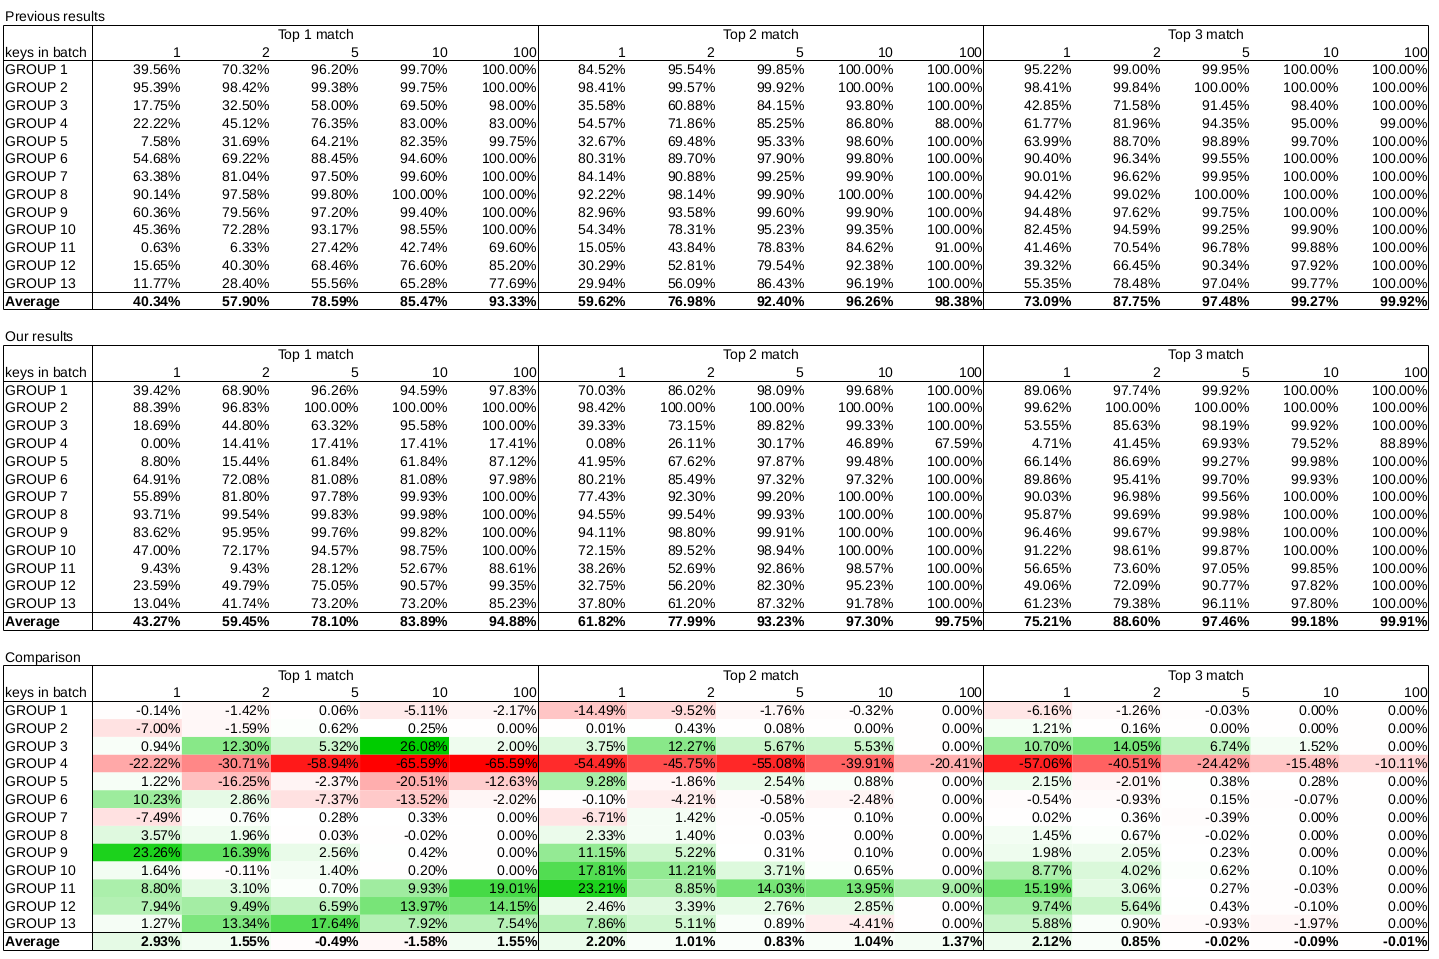
\includegraphics[width=\textwidth]{tex/images/results/comparison_13}
\caption{Comparison of results of CROCS lab and our model.}
\label{comparison-results}

\end{sidewaysfigure}

\noindent
When comparing the Naive Bayes model and the optimized neural network we can see, that:

\begin{itemize}

\item neural network model was able to adapt to the more complex dataset, when compared the scikit models. That is why the best-evaluated scikit model lags behind simple keras classifiers in accuracy.

\item our classifier was able to increase the overall accuracy by almost 3 \% when compared to the methods used by CROCS lab and almost 10 \% when compared to the best results achieved in \cite{thesis_sekan}.

\item a neural network is substantially better in classifying Group 9 (Yubikey 1 \& Infineon JTOP 80K). Given the recent problems with Infineon keys \cite{svenda_2}, discovering their keys with high probability could have been used for potential attack.

\item it performs slightly better on groups 8, 10, 11, 12, 13. 

\item when using a batch of 10+ keys, it can better differentiate groups 11, 12, beating Naive Bayes by 15 - 19 \% (group 11 contains very popular libraries like Crpyto++ and Microsoft crypto libraries).

\item when using a batch of 5+ keys, it can better differentiate group 13 beating Naive Bayes by 17.64 \% with accuracy 73.2 \%. The group 13 contains the highest number of sources, so the bigger success rate applies to a bigger set of sources.

\item the network has really struggled with the group 4. The main reason may have been insufficient data for this group (around 50K for 1024b and 200K for 512b). Therefore it was difficult to generate a balanced dataset containing this group.

\end{itemize}

\subsection*{Binary classifiers}

Based on the previous general model results we can see, that some groups can be detected with high probability even using one single key. We tried to train binary classifiers to differentiate these classes better:

\begin{figure}[H]

%first line
\begin{subfigure}{.33\textwidth}
  \centering
  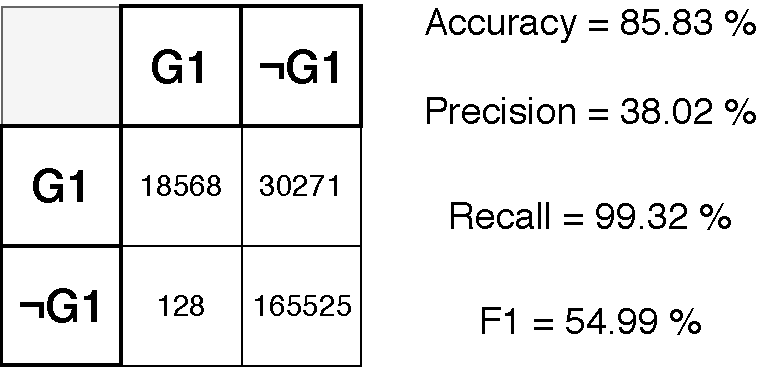
\includegraphics[width=\textwidth]{tex/images/results/rese_g1}  
\end{subfigure}%
\begin{subfigure}{.33\textwidth}
  \centering
  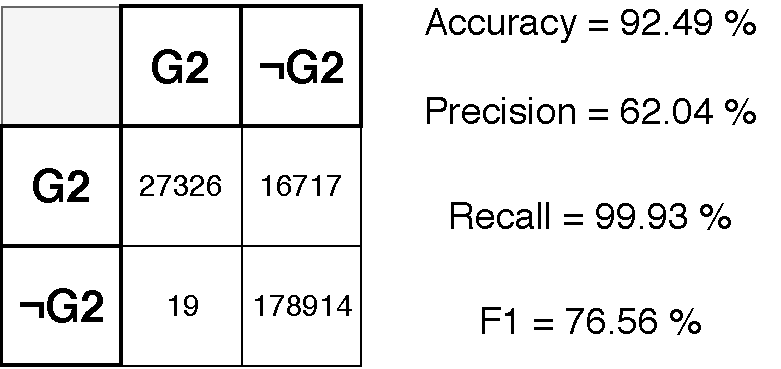
\includegraphics[width=\textwidth]{tex/images/results/rese_g2}
\end{subfigure}
\begin{subfigure}{.33\textwidth}
  \centering
  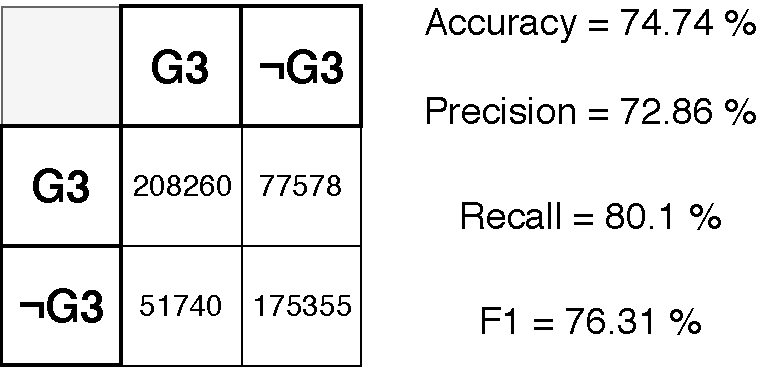
\includegraphics[width=\textwidth]{tex/images/results/rese_g3}
\end{subfigure}

\vspace{3mm}
%second line
\begin{subfigure}{.33\textwidth}
  \centering
  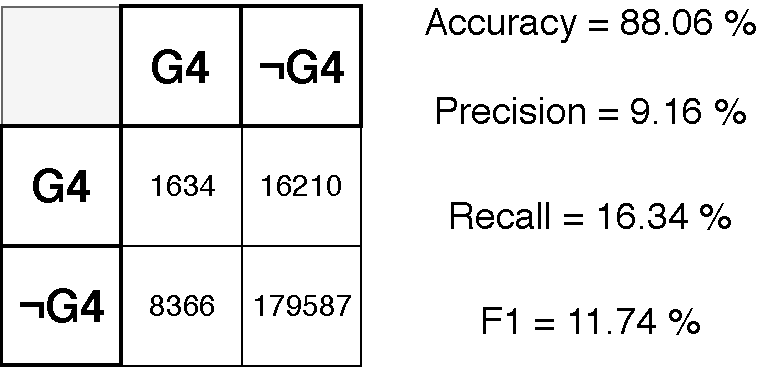
\includegraphics[width=\textwidth]{tex/images/results/rese_g4}  
\end{subfigure}%
\begin{subfigure}{.33\textwidth}
  \centering
  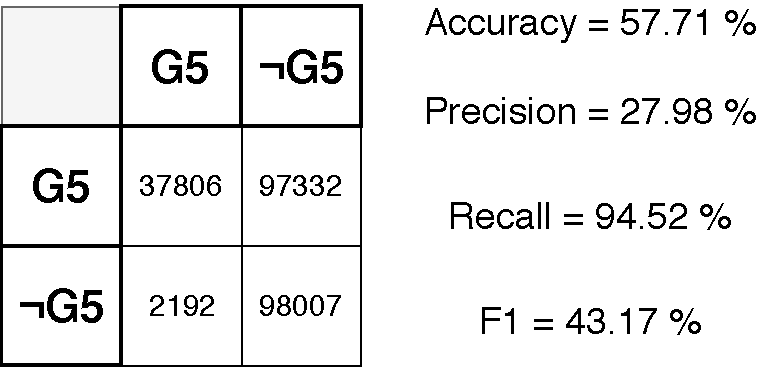
\includegraphics[width=\textwidth]{tex/images/results/rese_g5}
\end{subfigure}
\begin{subfigure}{.33\textwidth}
  \centering
  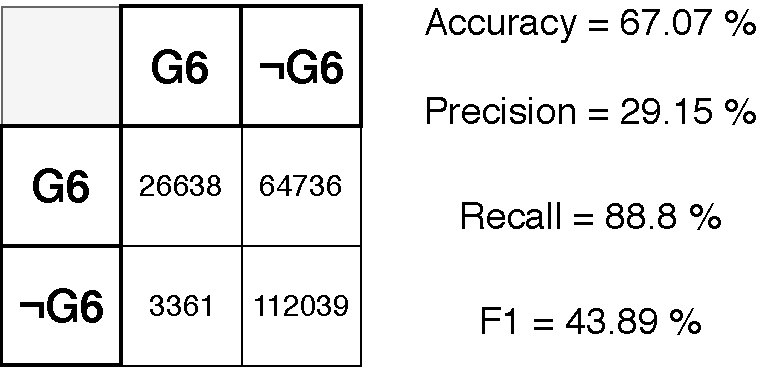
\includegraphics[width=\textwidth]{tex/images/results/rese_g6}
\end{subfigure}

\vspace{3mm}
%third line
\begin{subfigure}{.33\textwidth}
  \centering
  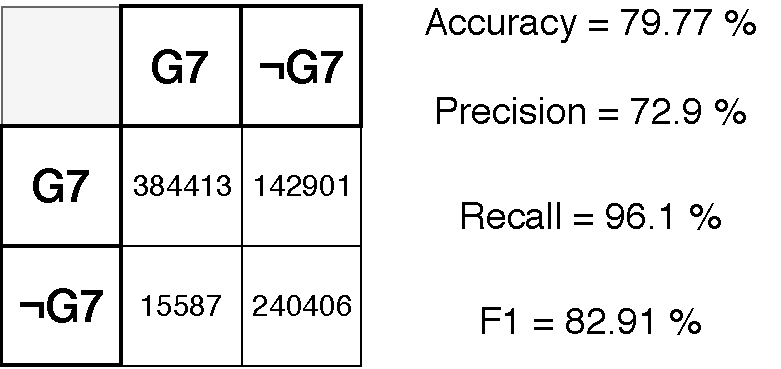
\includegraphics[width=\textwidth]{tex/images/results/rese_g7}  
\end{subfigure}%
\begin{subfigure}{.33\textwidth}
  \centering
  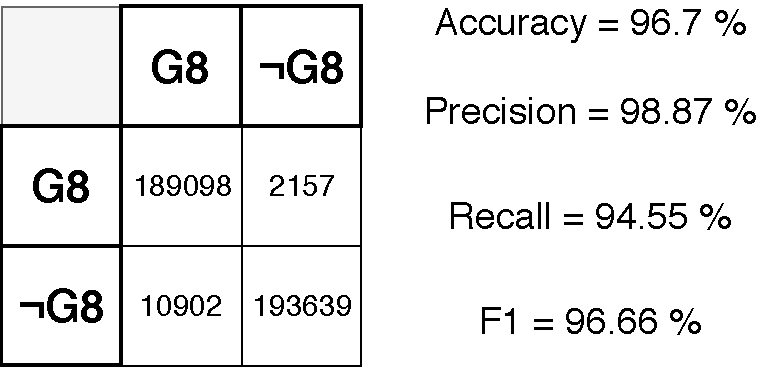
\includegraphics[width=\textwidth]{tex/images/results/rese_g8}
\end{subfigure}
\begin{subfigure}{.33\textwidth}
  \centering
  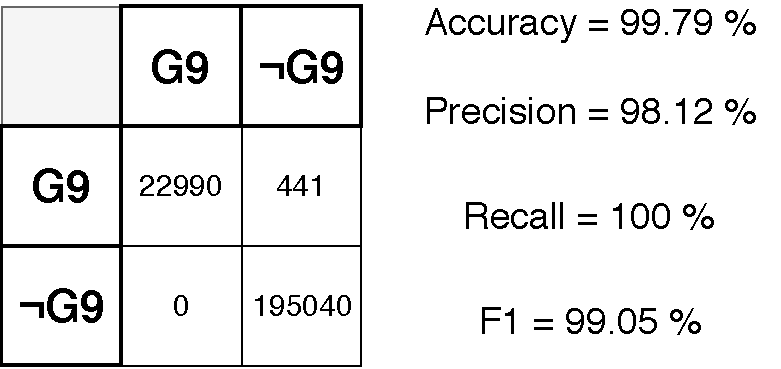
\includegraphics[width=\textwidth]{tex/images/results/rese_g9}
\end{subfigure}

\vspace{3mm}
%fourth line
\begin{subfigure}{.33\textwidth}
  \centering
  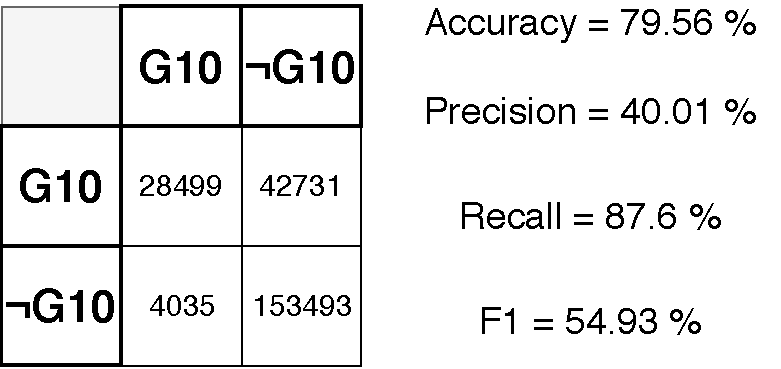
\includegraphics[width=\textwidth]{tex/images/results/rese_g10}  
\end{subfigure}%
\begin{subfigure}{.33\textwidth}
  \centering
  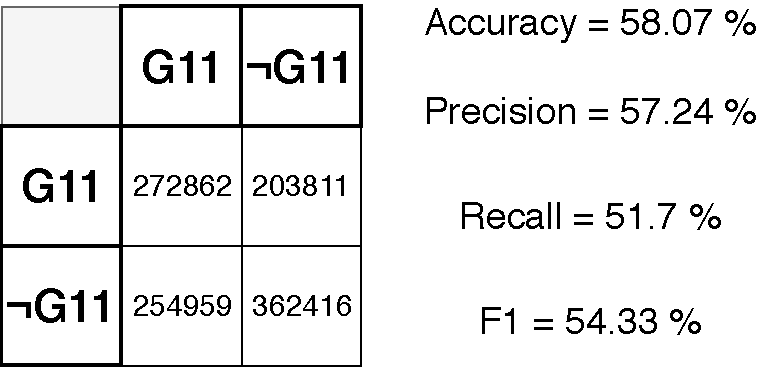
\includegraphics[width=\textwidth]{tex/images/results/rese_g11}
\end{subfigure}
\begin{subfigure}{.33\textwidth}
  \centering
  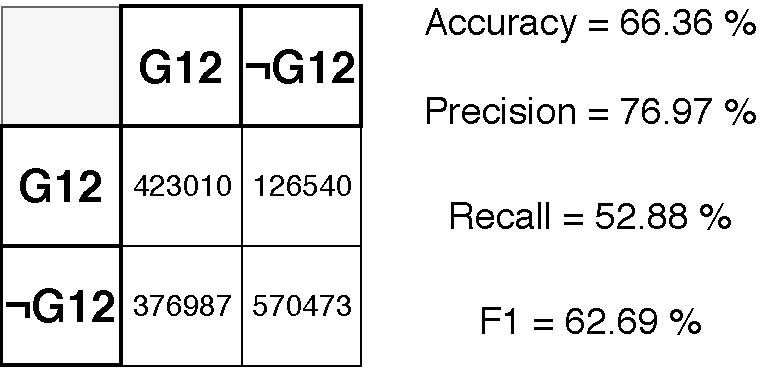
\includegraphics[width=\textwidth]{tex/images/results/rese_g12}
\end{subfigure}

\vspace{3mm}
%last line
\begin{subfigure}{.33\textwidth}
  \centering
  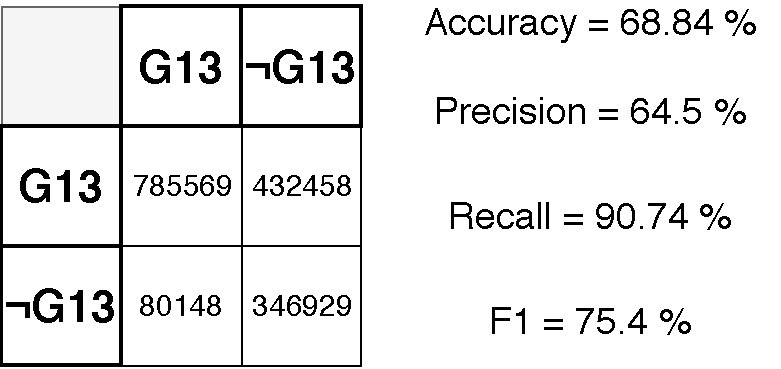
\includegraphics[width=\textwidth]{tex/images/results/rese_g13}  
\end{subfigure}%

\caption{Confusion matrices and metrics for 13 classifiers for each group trained individually.}

\end{figure}

\noindent
These results are comparable to the observations from the previous trial:

\begin{itemize}

\item the network completely fails to detect group 4 (even worse than random guessing)
\item it is more or less equal to random guessing with group 11
\item groups 1, 2, 5, 6, 7, 10 and 13 have relatively low precision leading to the higher number of false positives
\item the results for the biggest groups 7, 12 and 13 are more promising. It shows, that we can differentiate them better with accuracy and precision above 65 to 70 \%
\item group 2 can be well distinguished
\item group 8 is detected reliably (the reason is the first MSB being 0)
\item group 9 is detected reliably (the reasons are the moduli 11, 13, 17 and 19). However, the binary classifier overfitted to the small dataset introducing some ratio of false positives.

\end{itemize}

Given the fact that every classifier can be trained individually, we obtained the best results when putting them all together in the voting process. The same input was fed to 13 different binary classifiers, that outputted the probability, that the key belongs to the respective group. The classifier with the highest probability was voted as a winner.

We ran the voting classifier on the uniformly distributed dataset of 13 groups of bit length 1024. Table \ref{table-binary-voter} shows the obtained results. The notable observations of this run are:

\begin{itemize}

\item the overall accuracy is 4.94 \% higher than naive Bayes
\item the classifier gets more successful in identifying the large group 13, with the accuracy of 22.95 \% on the first guess and 73.21 \% when considering first top 3 results. This is almost 18 \% better than the result of naive Bayes and 12 \% better than our previous model.
\item it can detect group 8 with more accuracy (3.5 \% higher)
\item it overfitted group 9 (because of its size). Nevertheless, we identified, that this is the only group, that has bias modulo 11, 13, 17 and 19. We suppose that this classifier would perform well even on a bigger sample of this group\footnote{Group 9 contains Infineon chips, which were liable to attack as reported in \cite{svenda_2}. The correct classification of such group could be useful for the potential attacker.}. 

\end{itemize}

\begin{table}[h]
\centering
\begin{tabular}{| r | c | c | c | r | }
\hline
  Group & Top 1 match & Top 2 match & Top 3 match & \# of keys \\
  \hline
 1 & 58.30 \% & 89.20 \% & 97.06 \% & 93482 \\
 2 & 85.57 \% & 98.02 \% & 99.62 \% & 136727 \\
 3 & 15.28 \% & 32.07 \% & 52.50 \% & 200000 \\
 4 & 47.96 \% & 59.15 \% & 64.03 \% & 50000 \\
 5 & 39.82 \% & 69.73 \% & 85.47 \% & 200000 \\
 6 & 49.81 \% & 74.32 \% & 86.73 \% & 150000 \\
 7 & 55.21 \% & 76.15 \% & 90.36 \% & 200000 \\
 8 & 93.54 \% & 94.81 \% & 95.74 \% & 200000 \\
 9 & 100 \% & 100 \% & 100 \% & 114955 \\
 10 & 33.22 \% & 57.60 \% & 79.44 \% & 129347 \\
 11 & 0.34 \% & 23.59 \% & 47.16 \% & 189110 \\
 12 & 25.04 \% & 28.95 \% & 42.07 \% & 199990 \\
 13 & 22.95 \% & 53.84 \% & 73.21 \% & 191658 \\
 \hline
TOTAL & 45.28 \% & 63.21 \% & 76.32 \% & 2055269 \\
\hline

\end{tabular}
\caption{Accuracy table for a voting classifier of binary classifiers.}
\label{table-binary-voter}
\end{table}

The voting classifier performs better in almost every aspect than the previous one apart from groups 6, 10 and 11, for which the user could use rather the first one. If we also included the CROCS's naive bayes classifier for classifying group 2 (in which it is superior to both of our classifiers), we would get even more accurate predictions.

\subsection*{Group spliting}

As the last step, we tried even more precise classification between sources. We aimed to split at least one of the 13 groups. In the first approach, we ran the models on the huge dataset with 64 individual sources. In the second one, we took sources only from a single group and tried to classify them within it. We repeated it for each group.

However, when running several proven models on each group, the results showed as expected the uniform distribution in classification within the group, as the sources in one group shared the same distribution on the features. The network is not able to differentiate between them and is performing with the same results as random guessing. We suppose that the sources within each group share the same implementation steps that affect the distribution on bits in the public key and the distribution on the remainders modulo up to 30.


  \chapter{Conclusion}

In this thesis, we studied the use of neural networks in the classification process of public keys in RSA implementations. The work served as an extension of already ongoing research of CROCS lab in this field. 

We performed a detailed distributed analysis of the given dataset and found out different distributions on the six most significant bits which we presented in figure \ref{figure-table-bit-analysis}. Furthermore, our modular analysis (figure \ref{figure-mod-analysis}) supported the results presented by CROCS team.

A significant part of this thesis was the design of an application, capable of working with the given dataset. As there is an assumption that this application will be further used in CROCS research to try out new classification techniques, we focused on extensibility and efficiency. We implemented an interface that simplifies the training process as it isolates the data fetching to the model as a different logic. The models are accessible via the common interface, which makes new model integrations easier.

Using our framework, we methodologically compared the traditional methods and neural networks when classifying public keys. Our results showed the limitations in using traditional classifiers, especially with bigger datasets.

The first neural network was trained and optimized using a grid search technique. The task was too complex for the local machine. Thus it had to be trained on CESNET cloud. Our observations showed that the usage of activation or optimizer has little impact on the overall performance of the model. On the other hand, the uniform training dataset and topology were much more important. This optimized classifier performed better than Naive Bayes, especially on the large classes, where we had sufficient amount of data.

For the second model, we tried a different approach. Training individual binary classifiers and merging them in the voting process
turned out to be the best choice for groups with a sufficient amount of data. We could train the binary classifiers individually, optimizing every model by itself by customizing the train dataset and hyperparameters. The voting classifier was able to recognize large groups better compared to Naive Bayes. In practice, the voting model can recognize OpenSSL (group 7) keys\footnote{which make a majority key source in wide TLS scans} with 15 \% more precision than Naive Bayes. Furthermore, recently flawed Infineon chips (group 9) are detected with certainty over 99 \% just from one key, which is 40 \% better than previous results. Other popular libraries like Libgcrypt, OpenSSL FIPS, mbedTLS, etc. (from groups 12 and 13) are recognized with 10 \% more precision than Naive Bayes. 

As the last step, we tried to split the grouping even more precisely. However, using the existing features, the neural network is unable to do that. For the future work to improve these results, one can try different types of analysis like xor of all pairwise bits on one key. This process would need to be optimized though, as there are $\mathcal{O}(n^2)$ combinations for just one key only. The working voting classifier can be further optimized by training more accurate binary classifiers within the model on larger datasets. Also, one could experiment by adding a hidden layer on top. Other new models can also be included in the application.

  % \chapter{Notes}

\textbf{PIPELINE}
\begin{itemize}

\item dataset
\item key batch available
\item set of scripts over dataset
\item features from paper [Svenda2]
\item analysis of dataset (distributions of moduli)
\item feature engineering
\item different models (Scikit-learn models, keras models)
\item better results than svenda
\item needed optimization (usage of python generators) to be able to work with huge dataset in memory
\item this leads to better usage o metacentrum as well
\item next step was to split up the dataset into sources only and check this
\item split and merge groups (especially G13)
\item g15 binary classifier
\item yubikey binary classifier (same chip for infineon/yubikey)
\item sampling of training dataset 
\item Scripts to work with dataset (url)
\item preprocessed dataset (url) and final models git
\item every used model theory (multilayer perceptron, binary classifier, deep learning)
\item pandas, keras docs
\item similar work (mention Svenda papers, THESIS1, THESIS2)

\item implementation chapter (with dataset section)
\item metacentrum


\end{itemize}
  \printbibliography
  \appendix
  \chapter{Archive structure}

\begin{itemize}

\item \textbf{TODO} dataset cloud url
\item \textbf{TODO} tree

\end{itemize}


  \chapter{dataset}
\label{appendix-dataset}

\begin{table}[H]
\centering
\begin{tabular}{l|l|l|l|l|l|}
\hline
\multicolumn{1}{|l|}{\textbf{\#}}                         & \textbf{Source}              & \textbf{512}      & \textbf{1024}     & \textbf{2048}    & \textbf{Total}                             \\ \hline
\rowcolor[HTML]{FFCCC9} 
\multicolumn{1}{|l|}{\cellcolor[HTML]{FFCCC9}\textbf{1}}  & G\&D SmartCafe 3.2           & 126344            & 93482             & 0                & 219826                                     \\
\rowcolor[HTML]{FFCCC9} 
\multicolumn{1}{|l|}{\cellcolor[HTML]{FFCCC9}\textbf{2}}  & G\&D SmartCafe 4.x           & 2075779           & 50000             & 0                & 2125779                                    \\
\rowcolor[HTML]{FFCCC9} 
\multicolumn{1}{|l|}{\cellcolor[HTML]{FFCCC9}\textbf{3}}  & G\&D SmartCafe 6.0           & 200000            & 86727             & 0                & 286727                                     \\
\rowcolor[HTML]{FFFC9E} 
\multicolumn{1}{|l|}{\cellcolor[HTML]{FFFC9E}\textbf{4}}  & GNU Crypto 2.0.1             & 1320000           & 1320000           & 132000           & 2772000                                    \\
\rowcolor[HTML]{FFCCC9} 
\multicolumn{1}{|l|}{\cellcolor[HTML]{FFCCC9}\textbf{5}}  & Gemalto GXP E64              & 200000            & 50000             & 0                & 250000                                     \\
\rowcolor[HTML]{FFCCC9} 
\multicolumn{1}{|l|}{\cellcolor[HTML]{FFCCC9}\textbf{6}}  & NXP J2A080                   & 3000000           & 50000             & 0                & 3050000                                    \\
\rowcolor[HTML]{FFCCC9} 
\multicolumn{1}{|l|}{\cellcolor[HTML]{FFCCC9}\textbf{7}}  & NXP J2A081                   & 2623990           & 50000             & 0                & 2673990                                    \\
\rowcolor[HTML]{FFCCC9} 
\multicolumn{1}{|l|}{\cellcolor[HTML]{FFCCC9}\textbf{8}}  & NXP J3A081                   & 2990413           & 50000             & 0                & 3040413                                    \\
\rowcolor[HTML]{FFCCC9} 
\multicolumn{1}{|l|}{\cellcolor[HTML]{FFCCC9}\textbf{9}}  & NXP JCOP 41 V2.2.1           & 993640            & 50000             & 0                & 1043640                                    \\
\rowcolor[HTML]{FFCCC9} 
\multicolumn{1}{|l|}{\cellcolor[HTML]{FFCCC9}\textbf{10}} & Oberthur Cosmo Dual 72K      & 152773            & 150000            & 0                & 302773                                     \\
\rowcolor[HTML]{FFFC9E} 
\multicolumn{1}{|l|}{\cellcolor[HTML]{FFFC9E}\textbf{11}} & OpenSSL 0.9.7                & 1100000           & 1100000           & 110000           & 2310000                                    \\
\rowcolor[HTML]{FFFC9E} 
\multicolumn{1}{|l|}{\cellcolor[HTML]{FFFC9E}\textbf{12}} & OpenSSL 1.0.2g               & 2200000           & 2200000           & 220000           & 4620000                                    \\
\rowcolor[HTML]{FFFC9E} 
\multicolumn{1}{|l|}{\cellcolor[HTML]{FFFC9E}\textbf{13}} & OpenSSL 1.0.2k               & 1100000           & 1100000           & 110000           & 2310000                                    \\
\rowcolor[HTML]{FFFC9E} 
\multicolumn{1}{|l|}{\cellcolor[HTML]{FFFC9E}\textbf{14}} & OpenSSL 1.1.0e               & 1100000           & 1100000           & 110000           & 2310000                                    \\
\rowcolor[HTML]{FFFC9E} 
\multicolumn{1}{|l|}{\cellcolor[HTML]{FFFC9E}\textbf{15}} & PGP SDK 4 FIPS               & 1239760           & 1369463           & 137655           & 2746878                                    \\
\rowcolor[HTML]{FFCCC9} 
\multicolumn{1}{|l|}{\cellcolor[HTML]{FFCCC9}\textbf{16}} & Infineon JTOP 80K            & 3000000           & 50000             & 0                & 3050000                                    \\
\rowcolor[HTML]{FFCCC9} 
\multicolumn{1}{|l|}{\cellcolor[HTML]{FFCCC9}\textbf{17}} & YubiKey 4                    & 0                 & 41671             & 0                & 41671                                      \\
\rowcolor[HTML]{FFCCC9} 
\multicolumn{1}{|l|}{\cellcolor[HTML]{FFCCC9}\textbf{18}} & YubiKey 4 Nano               & 0                 & 23284             & 0                & 23284                                      \\
\rowcolor[HTML]{FFCCC9} 
\multicolumn{1}{|l|}{\cellcolor[HTML]{FFCCC9}\textbf{19}} & NXP J2D081                   & 2387010           & 50000             & 0                & 2437010                                    \\
\rowcolor[HTML]{FFCCC9} 
\multicolumn{1}{|l|}{\cellcolor[HTML]{FFCCC9}\textbf{20}} & NXP J2E145G                  & 150000            & 100000            & 0                & 250000                                     \\
\rowcolor[HTML]{FFCCC9} 
\multicolumn{1}{|l|}{\cellcolor[HTML]{FFCCC9}\textbf{21}} & YubiKey NEO                  & 0                 & 12681             & 0                & 12681                                      \\
\rowcolor[HTML]{FFFC9E} 
\multicolumn{1}{|l|}{\cellcolor[HTML]{FFFC9E}\textbf{22}} & Bouncy Castle 1.54           & 2200000           & 2200000           & 220000           & 4620000                                    \\
\rowcolor[HTML]{FFFC9E} 
\multicolumn{1}{|l|}{\cellcolor[HTML]{FFFC9E}\textbf{23}} & Crypto++ 5.6.0               & 1100000           & 1100000           & 110000           & 2310000                                    \\
\rowcolor[HTML]{FFFC9E} 
\multicolumn{1}{|l|}{\cellcolor[HTML]{FFFC9E}\textbf{24}} & Crypto++ 5.6.3               & 2200000           & 2200000           & 220000           & 4620000                                    \\
\rowcolor[HTML]{FFFC9E} 
\multicolumn{1}{|l|}{\cellcolor[HTML]{FFFC9E}\textbf{25}} & Crypto++ 5.6.5               & 1100000           & 1100000           & 110000           & 2310000                                    \\
\rowcolor[HTML]{FFFC9E} 
\multicolumn{1}{|l|}{\cellcolor[HTML]{FFFC9E}\textbf{26}} & Libgcrypt 1.7.6 FIPS         & 10636             & 14110             & 12273            & 37019                                      \\
\rowcolor[HTML]{FFFC9E} 
\multicolumn{1}{|l|}{\cellcolor[HTML]{FFFC9E}\textbf{27}} & Microsoft CryptoAPI          & 1100000           & 1098997           & 110000           & 2308997                                    \\
\rowcolor[HTML]{FFFC9E} 
\multicolumn{1}{|l|}{\cellcolor[HTML]{FFFC9E}\textbf{28}} & Microsoft CNG                & 1100000           & 1100000           & 120000           & 2320000                                    \\

\end{tabular}
\end{table}

\begin{table}[H]
\centering
\begin{tabular}{l|l|l|l|l|l|}
\hline
\multicolumn{1}{|l|}{\textbf{\#}}                         & \textbf{Source}              & \textbf{512}      & \textbf{1024}     & \textbf{2048}    & \textbf{Total}                             \\ \hline
\rowcolor[HTML]{FFFC9E} 
\multicolumn{1}{|l|}{\cellcolor[HTML]{FFFC9E}\textbf{29}} & Microsoft.NET                & 1100000           & 800000            & 136180           & 2036180                                    \\
\rowcolor[HTML]{FFFC9E} 
\multicolumn{1}{|l|}{\cellcolor[HTML]{FFFC9E}\textbf{30}} & Bouncy Castle 1.53           & 1100000           & 1100000           & 110000           & 2310000                                    \\
\rowcolor[HTML]{FFFC9E} 
\multicolumn{1}{|l|}{\cellcolor[HTML]{FFFC9E}\textbf{31}} & Cryptix JCE 20050328         & 1100000           & 1100000           & 110000           & 2310000                                    \\
\rowcolor[HTML]{FFFC9E} 
\multicolumn{1}{|l|}{\cellcolor[HTML]{FFFC9E}\textbf{32}} & FlexiProvider 1.7p7          & 1100000           & 1100000           & 110000           & 2310000                                    \\
\rowcolor[HTML]{9AFF99} 
\multicolumn{1}{|l|}{\cellcolor[HTML]{9AFF99}\textbf{33}} & Utimaco Security Server Se50 & 999999            & 666665            & 0                & 1666664                                    \\
\rowcolor[HTML]{FFFC9E} 
\multicolumn{1}{|l|}{\cellcolor[HTML]{FFFC9E}\textbf{34}} & Nettle 2.0                   & 1100000           & 1100000           & 110000           & 2310000                                    \\
\rowcolor[HTML]{FFFC9E} 
\multicolumn{1}{|l|}{\cellcolor[HTML]{FFFC9E}\textbf{35}} & PuTTY 0.67                   & 0                 & 1000000           & 0                & 1000000                                    \\
\rowcolor[HTML]{FFFC9E} 
\multicolumn{1}{|l|}{\cellcolor[HTML]{FFFC9E}\textbf{36}} & SunRsaSign OpenJDK 1.8       & 1100000           & 1100000           & 110000           & 2310000                                    \\
\rowcolor[HTML]{FFFC9E} 
\multicolumn{1}{|l|}{\cellcolor[HTML]{FFFC9E}\textbf{37}} & mbedTLS 0.10.0               & 1100000           & 1100000           & 110000           & 2310000                                    \\
\rowcolor[HTML]{FFFC9E} 
\multicolumn{1}{|l|}{\cellcolor[HTML]{FFFC9E}\textbf{38}} & mbedTLS 1.3.19               & 1100000           & 1100000           & 110000           & 2310000                                    \\
\rowcolor[HTML]{FFFC9E} 
\multicolumn{1}{|l|}{\cellcolor[HTML]{FFFC9E}\textbf{39}} & mbedTLS 2.2.1                & 2200000           & 2200000           & 220000           & 4620000                                    \\
\rowcolor[HTML]{FFFC9E} 
\multicolumn{1}{|l|}{\cellcolor[HTML]{FFFC9E}\textbf{40}} & mbedTLS 2.4.2                & 1100000           & 1100000           & 110000           & 2310000                                    \\
\rowcolor[HTML]{FFFC9E} 
\multicolumn{1}{|l|}{\cellcolor[HTML]{FFFC9E}\textbf{41}} & Botan 1.5.6                  & 1100000           & 1100000           & 110000           & 2310000                                    \\
\rowcolor[HTML]{FFFC9E} 
\multicolumn{1}{|l|}{\cellcolor[HTML]{FFFC9E}\textbf{42}} & Botan 1.11.29                & 2231840           & 1384780           & 122565           & 3739185                                    \\
\rowcolor[HTML]{FFFC9E} 
\multicolumn{1}{|l|}{\cellcolor[HTML]{FFFC9E}\textbf{43}} & Botan 2.1.0                  & 1100000           & 0                 & 110000           & 1210000                                    \\
\rowcolor[HTML]{FFFC9E} 
\multicolumn{1}{|l|}{\cellcolor[HTML]{FFFC9E}\textbf{44}} & Cryptlib 3.4.3               & 2200000           & 2200000           & 205788           & 4605788                                    \\
\rowcolor[HTML]{FFFC9E} 
\multicolumn{1}{|l|}{\cellcolor[HTML]{FFFC9E}\textbf{45}} & Cryptlib 3.4.3.1             & 1100000           & 1100000           & 96306            & 2296306                                    \\
\rowcolor[HTML]{FFCCC9} 
\multicolumn{1}{|l|}{\cellcolor[HTML]{FFCCC9}\textbf{46}} & Feitian JavaCOS A22          & 200000            & 100000            & 0                & 300000                                     \\
\rowcolor[HTML]{FFCCC9} 
\multicolumn{1}{|l|}{\cellcolor[HTML]{FFCCC9}\textbf{47}} & Feitian JavaCOS A40          & 200000            & 98568             & 0                & 298568                                     \\
\rowcolor[HTML]{FFCCC9} 
\multicolumn{1}{|l|}{\cellcolor[HTML]{FFCCC9}\textbf{48}} & Gemalto GCX4 72K             & 200000            & 50000             & 0                & 250000                                     \\
\rowcolor[HTML]{9AFF99} 
\multicolumn{1}{|l|}{\cellcolor[HTML]{9AFF99}\textbf{49}} & SafeNet Luna SA-1700         & 1000000           & 999999            & 180001           & 2180000                                    \\
\rowcolor[HTML]{FFFC9E} 
\multicolumn{1}{|l|}{\cellcolor[HTML]{FFFC9E}\textbf{50}} & LibTomCrypt 1.17             & 1100000           & 1100000           & 110000           & 2310000                                    \\
\rowcolor[HTML]{FFFC9E} 
\multicolumn{1}{|l|}{\cellcolor[HTML]{FFFC9E}\textbf{51}} & Libgcrypt 1.6.0              & 0                 & 2200000           & 0                & 2200000                                    \\
\rowcolor[HTML]{FFFC9E} 
\multicolumn{1}{|l|}{\cellcolor[HTML]{FFFC9E}\textbf{52}} & Libgcrypt 1.6.5              & 2200000           & 3300000           & 220000           & 5720000                                    \\
\rowcolor[HTML]{FFFC9E} 
\multicolumn{1}{|l|}{\cellcolor[HTML]{FFFC9E}\textbf{53}} & Libgcrypt 1.7.6              & 2200000           & 2200000           & 220000           & 4620000                                    \\
\rowcolor[HTML]{FFFC9E} 
\multicolumn{1}{|l|}{\cellcolor[HTML]{FFFC9E}\textbf{54}} & Libgcrypt 1.6.0 FIPS         & 0                 & 2200000           & 0                & 2200000                                    \\
\rowcolor[HTML]{FFFC9E} 
\multicolumn{1}{|l|}{\cellcolor[HTML]{FFFC9E}\textbf{55}} & Libgcrypt 1.6.5 FIPS         & 1100000           & 3300000           & 110000           & 4510000                                    \\
\rowcolor[HTML]{FFFC9E} 
\multicolumn{1}{|l|}{\cellcolor[HTML]{FFFC9E}\textbf{56}} & Nettle 3.2                   & 2200000           & 2200000           & 220000           & 4620000                                    \\
\rowcolor[HTML]{FFFC9E} 
\multicolumn{1}{|l|}{\cellcolor[HTML]{FFFC9E}\textbf{57}} & Nettle 3.3                   & 1100000           & 1100000           & 110000           & 2310000                                    \\
\rowcolor[HTML]{FFCCC9} 
\multicolumn{1}{|l|}{\cellcolor[HTML]{FFCCC9}\textbf{58}} & Oberthur Cosmo 64            & 0                 & 121750            & 0                & 121750                                     \\

\end{tabular}
\end{table}

\begin{table}[H]
\centering
\begin{tabular}{l|l|l|l|l|l|}
\hline
\multicolumn{1}{|l|}{\textbf{\#}}                         & \textbf{Source}              & \textbf{512}      & \textbf{1024}     & \textbf{2048}    & \textbf{Total}                             \\ \hline
\rowcolor[HTML]{FFFC9E} 
\multicolumn{1}{|l|}{\cellcolor[HTML]{FFFC9E}\textbf{59}} & OpenSSL 2.0.12 FIPS          & 2200000           & 2200000           & 220000           & 4620000                                    \\
\rowcolor[HTML]{FFFC9E} 
\multicolumn{1}{|l|}{\cellcolor[HTML]{FFFC9E}\textbf{60}} & OpenSSL 1.0.2k FIPS          & 0                 & 1100000           & 0                & 1100000                                    \\
\rowcolor[HTML]{FFFC9E} 
\multicolumn{1}{|l|}{\cellcolor[HTML]{FFFC9E}\textbf{61}} & PGP SDK 4                    & 1890698           & 1650207           & 112303           & 3653208                                    \\
\rowcolor[HTML]{FFFC9E} 
\multicolumn{1}{|l|}{\cellcolor[HTML]{FFFC9E}\textbf{62}} & WolfSS 2.0rc1                & 1100000           & 1100000           & 110000           & 2310000                                    \\
\rowcolor[HTML]{FFFC9E} 
\multicolumn{1}{|l|}{\cellcolor[HTML]{FFFC9E}\textbf{63}} & WolfSSL 3.9.0                & 2200000           & 2200000           & 220000           & 4620000                                    \\
\rowcolor[HTML]{FFFC9E} 
\multicolumn{1}{|l|}{\cellcolor[HTML]{FFFC9E}\textbf{64}} & WolfSSL 3.10.2               & 1100000           & 1100000           & 110000           & 2310000                                    \\ \hline
                                                          & \textit{Total}               & \textit{75592882} & \textit{65482384} & \textit{5545071} & \cellcolor[HTML]{FFFFFF}\textit{146620337} \\ \cline{2-6} 
\end{tabular}

\caption{Complete dataset table, the yellow rows are software libraries, the red rows represent cards and the green ones represent HSM's}
\end{table}

  \chapter{Analysis}

\label{appendix-analysis}

\section{Modular analysis}
\label{appendix-modular-analysis}

\begin{figure}[ht]
\centering
\begin{adjustbox}{minipage=\linewidth,scale=0.8}
\begin{subfigure}{0.45\textwidth}
	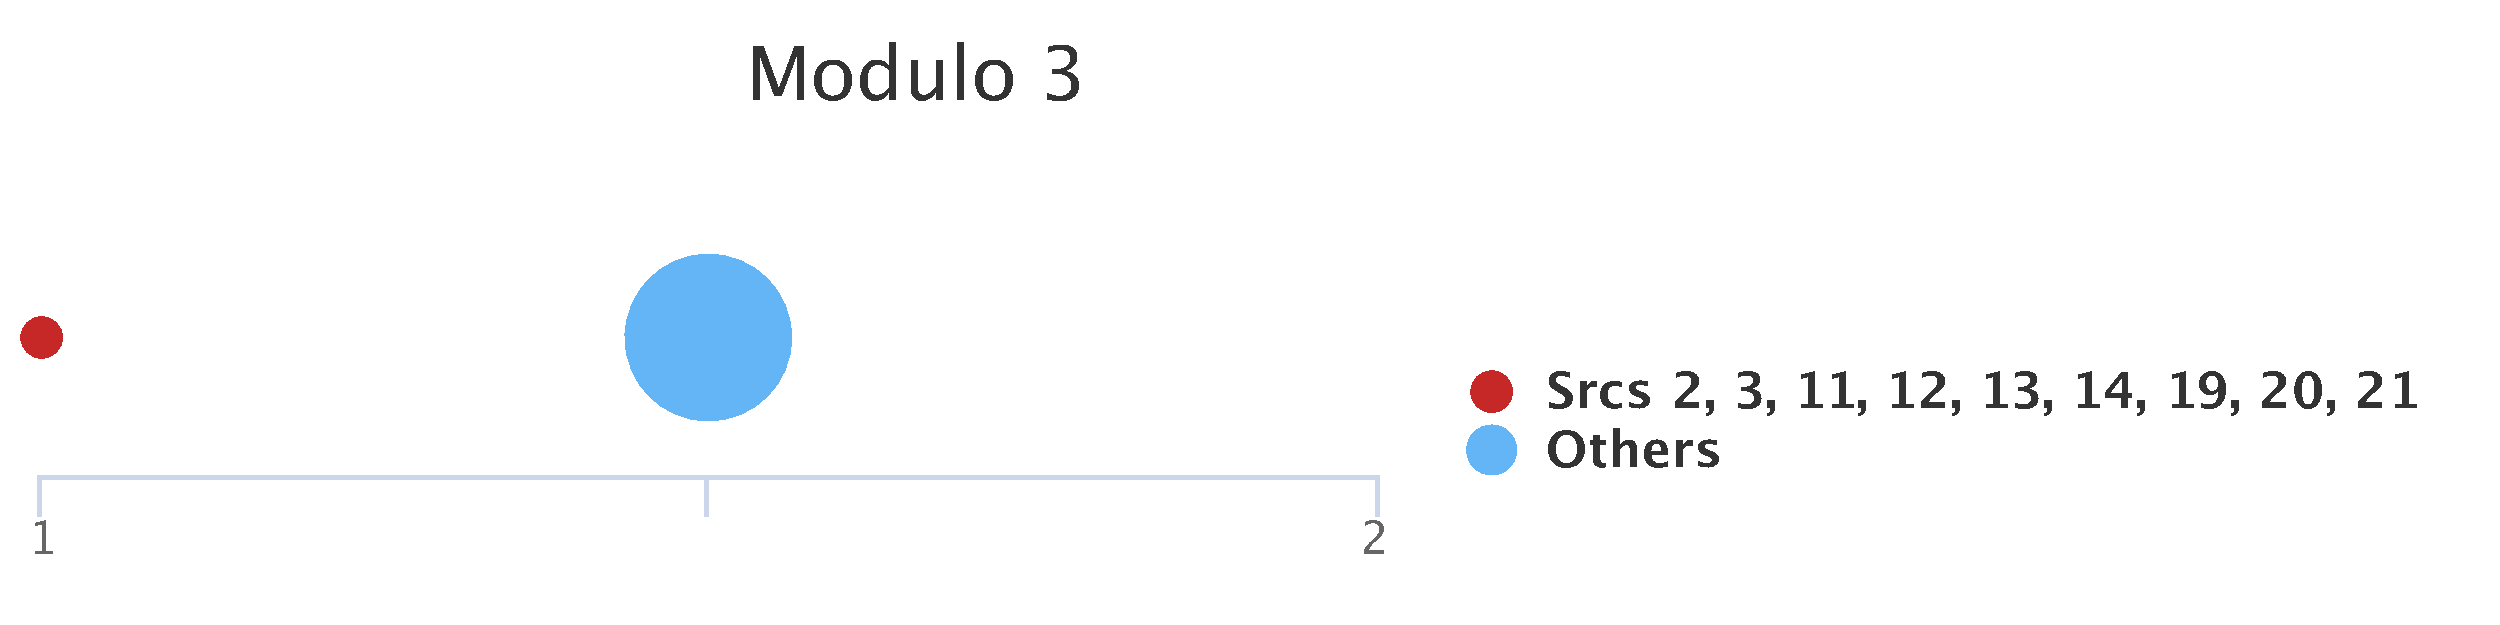
\includegraphics[width=\linewidth]{tex/images/analysis/mod3}
\end{subfigure}
\hfill
\begin{subfigure}{0.45\textwidth}
	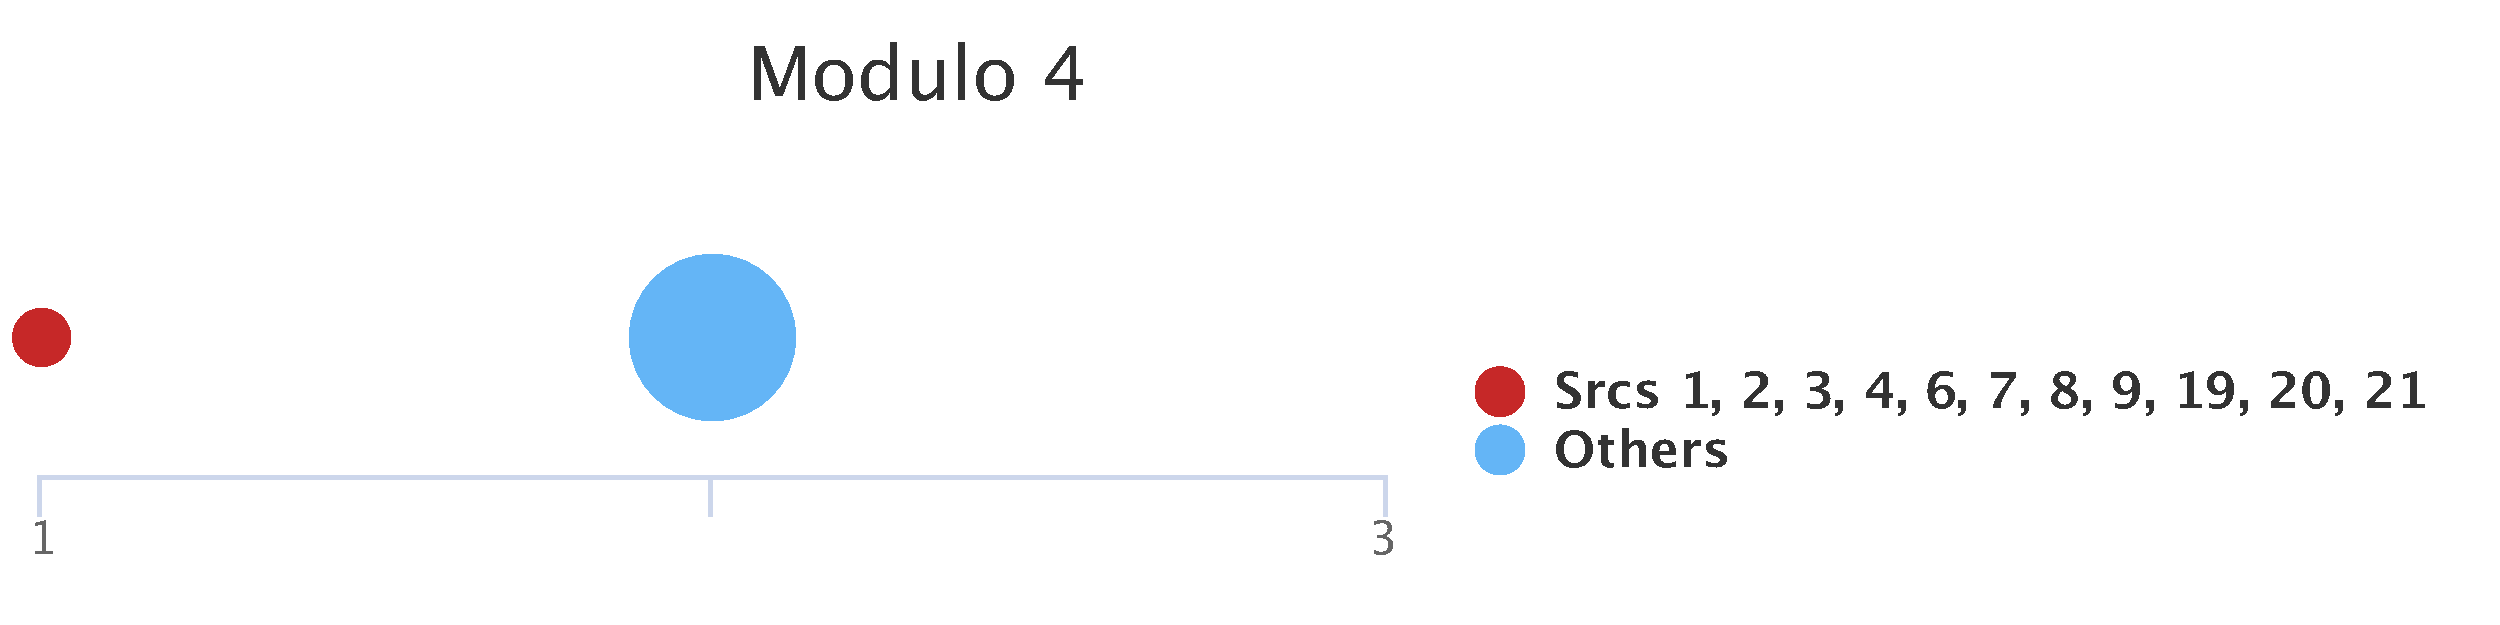
\includegraphics[width=\linewidth]{tex/images/analysis/mod4}
\end{subfigure}\\

\begin{subfigure}{0.45\textwidth}
	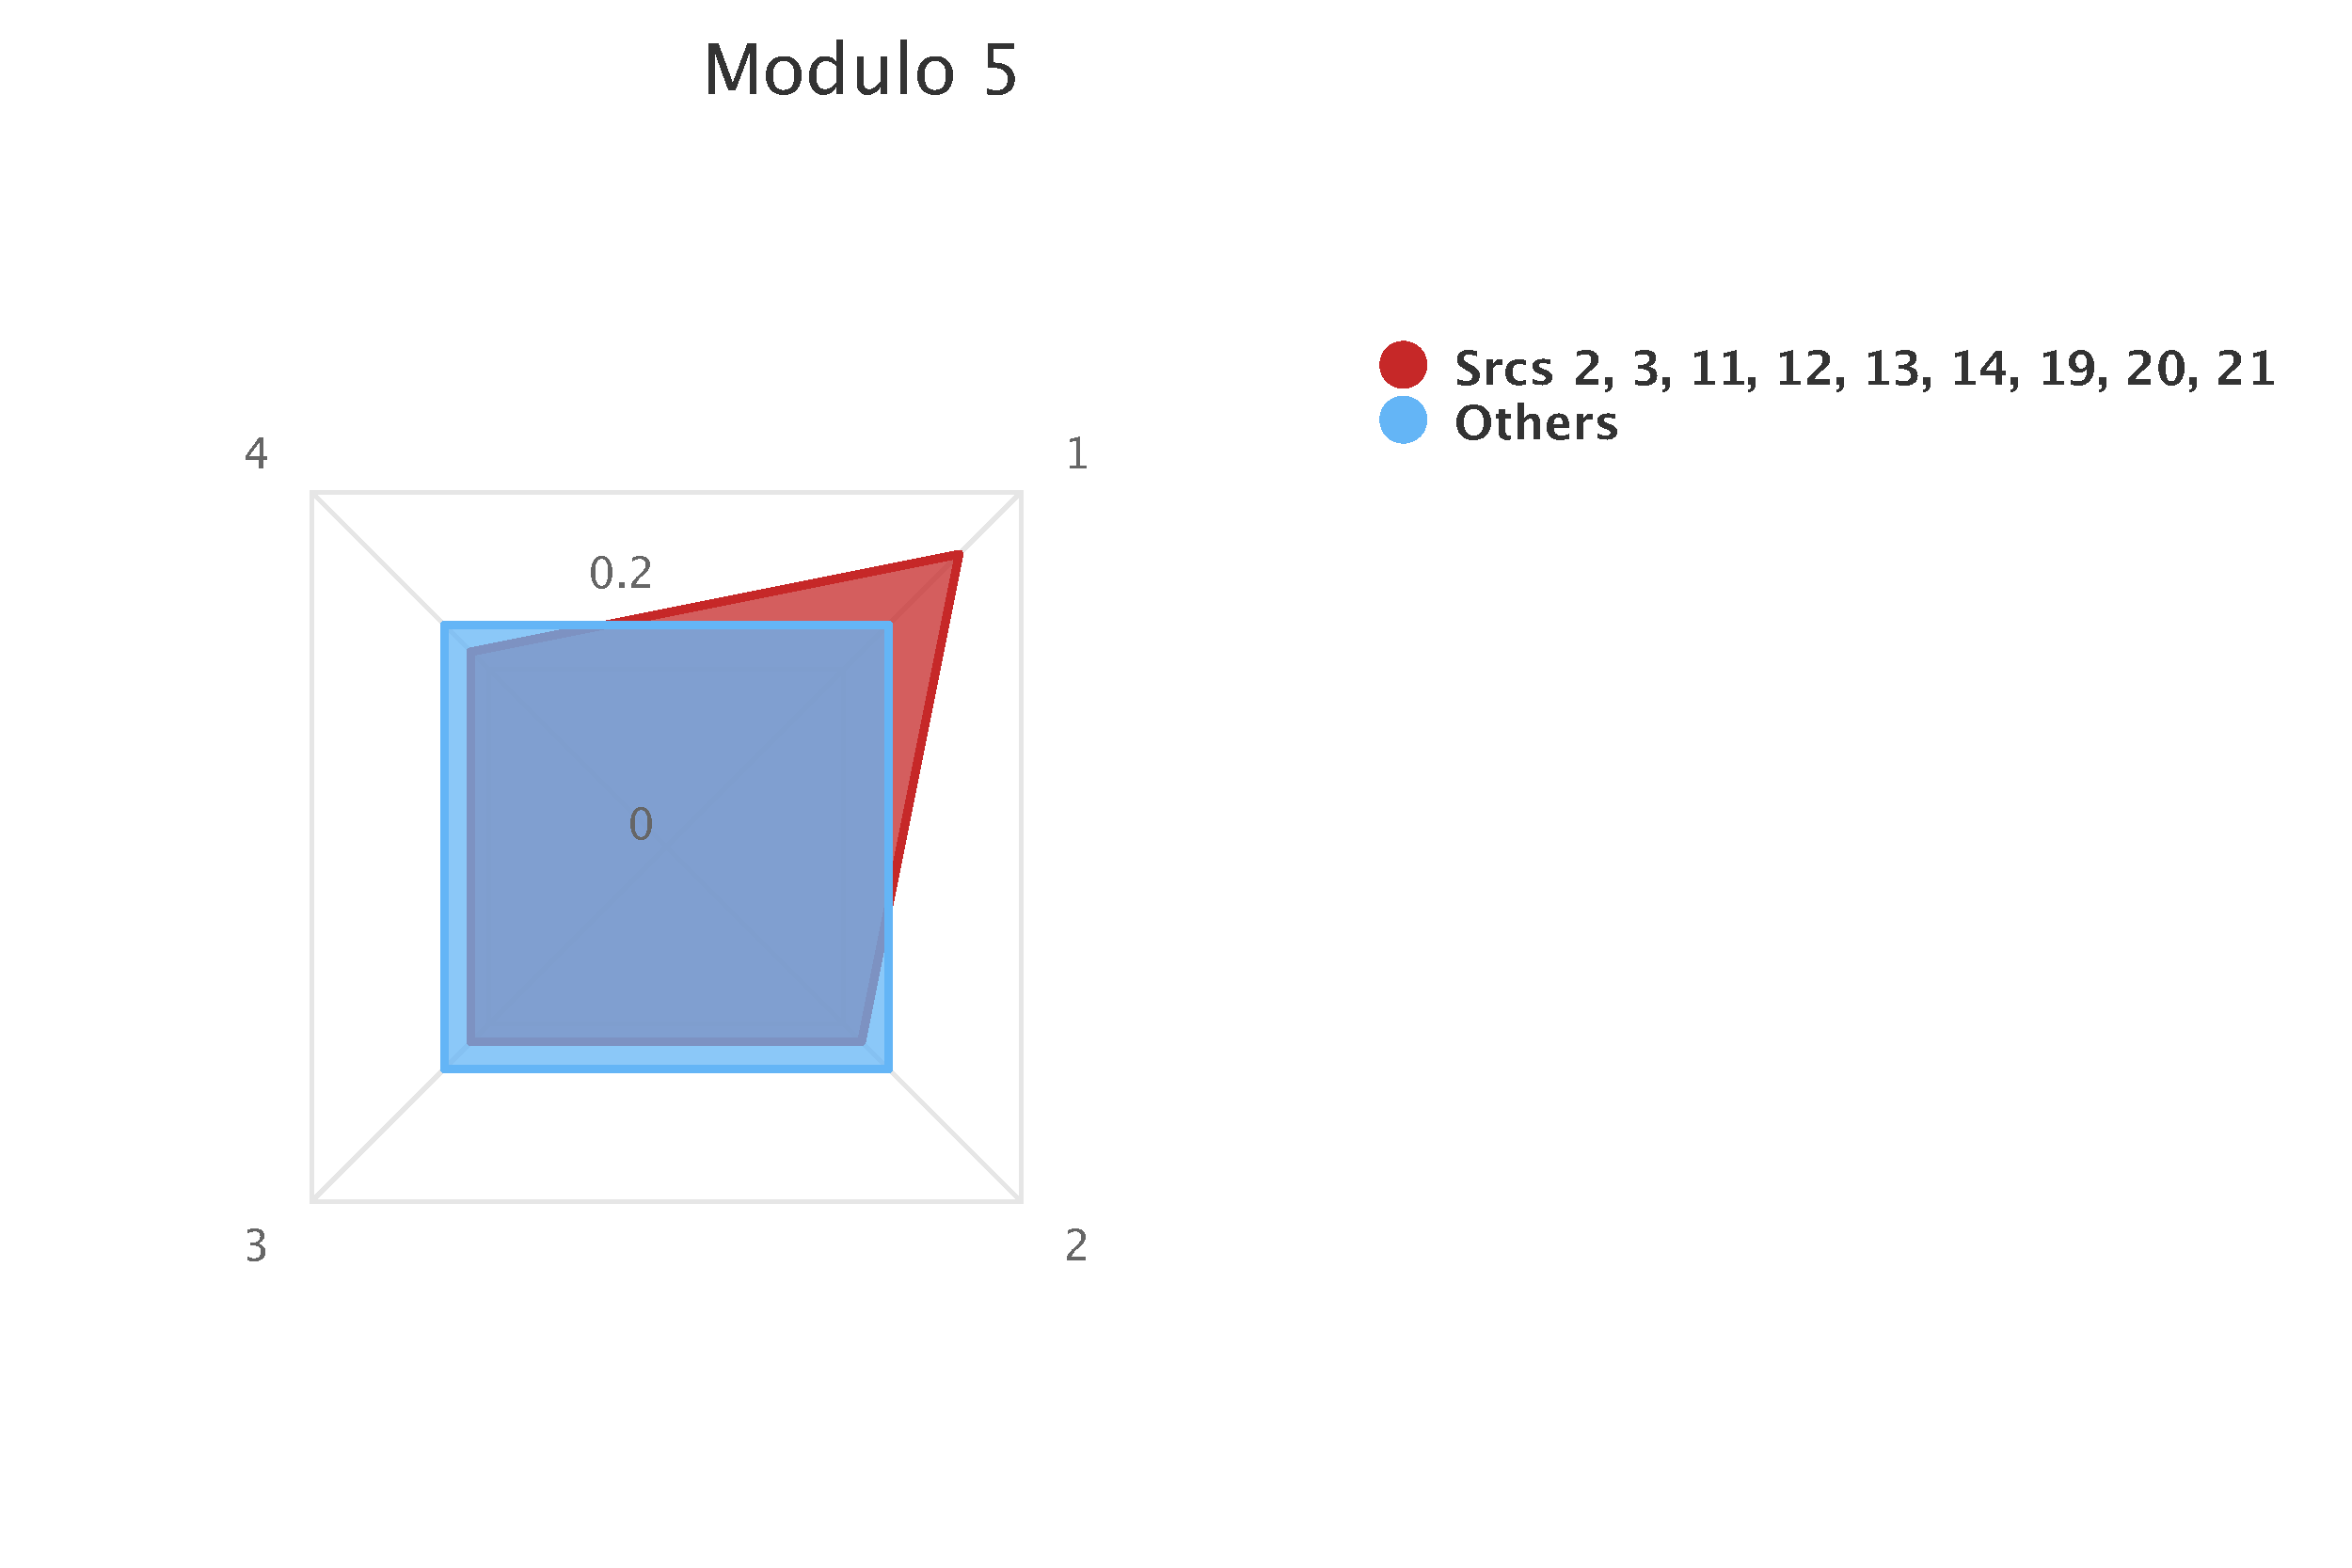
\includegraphics[width=\linewidth]{tex/images/analysis/mod5}
\end{subfigure}
\hfill
\begin{subfigure}{0.45\textwidth}
	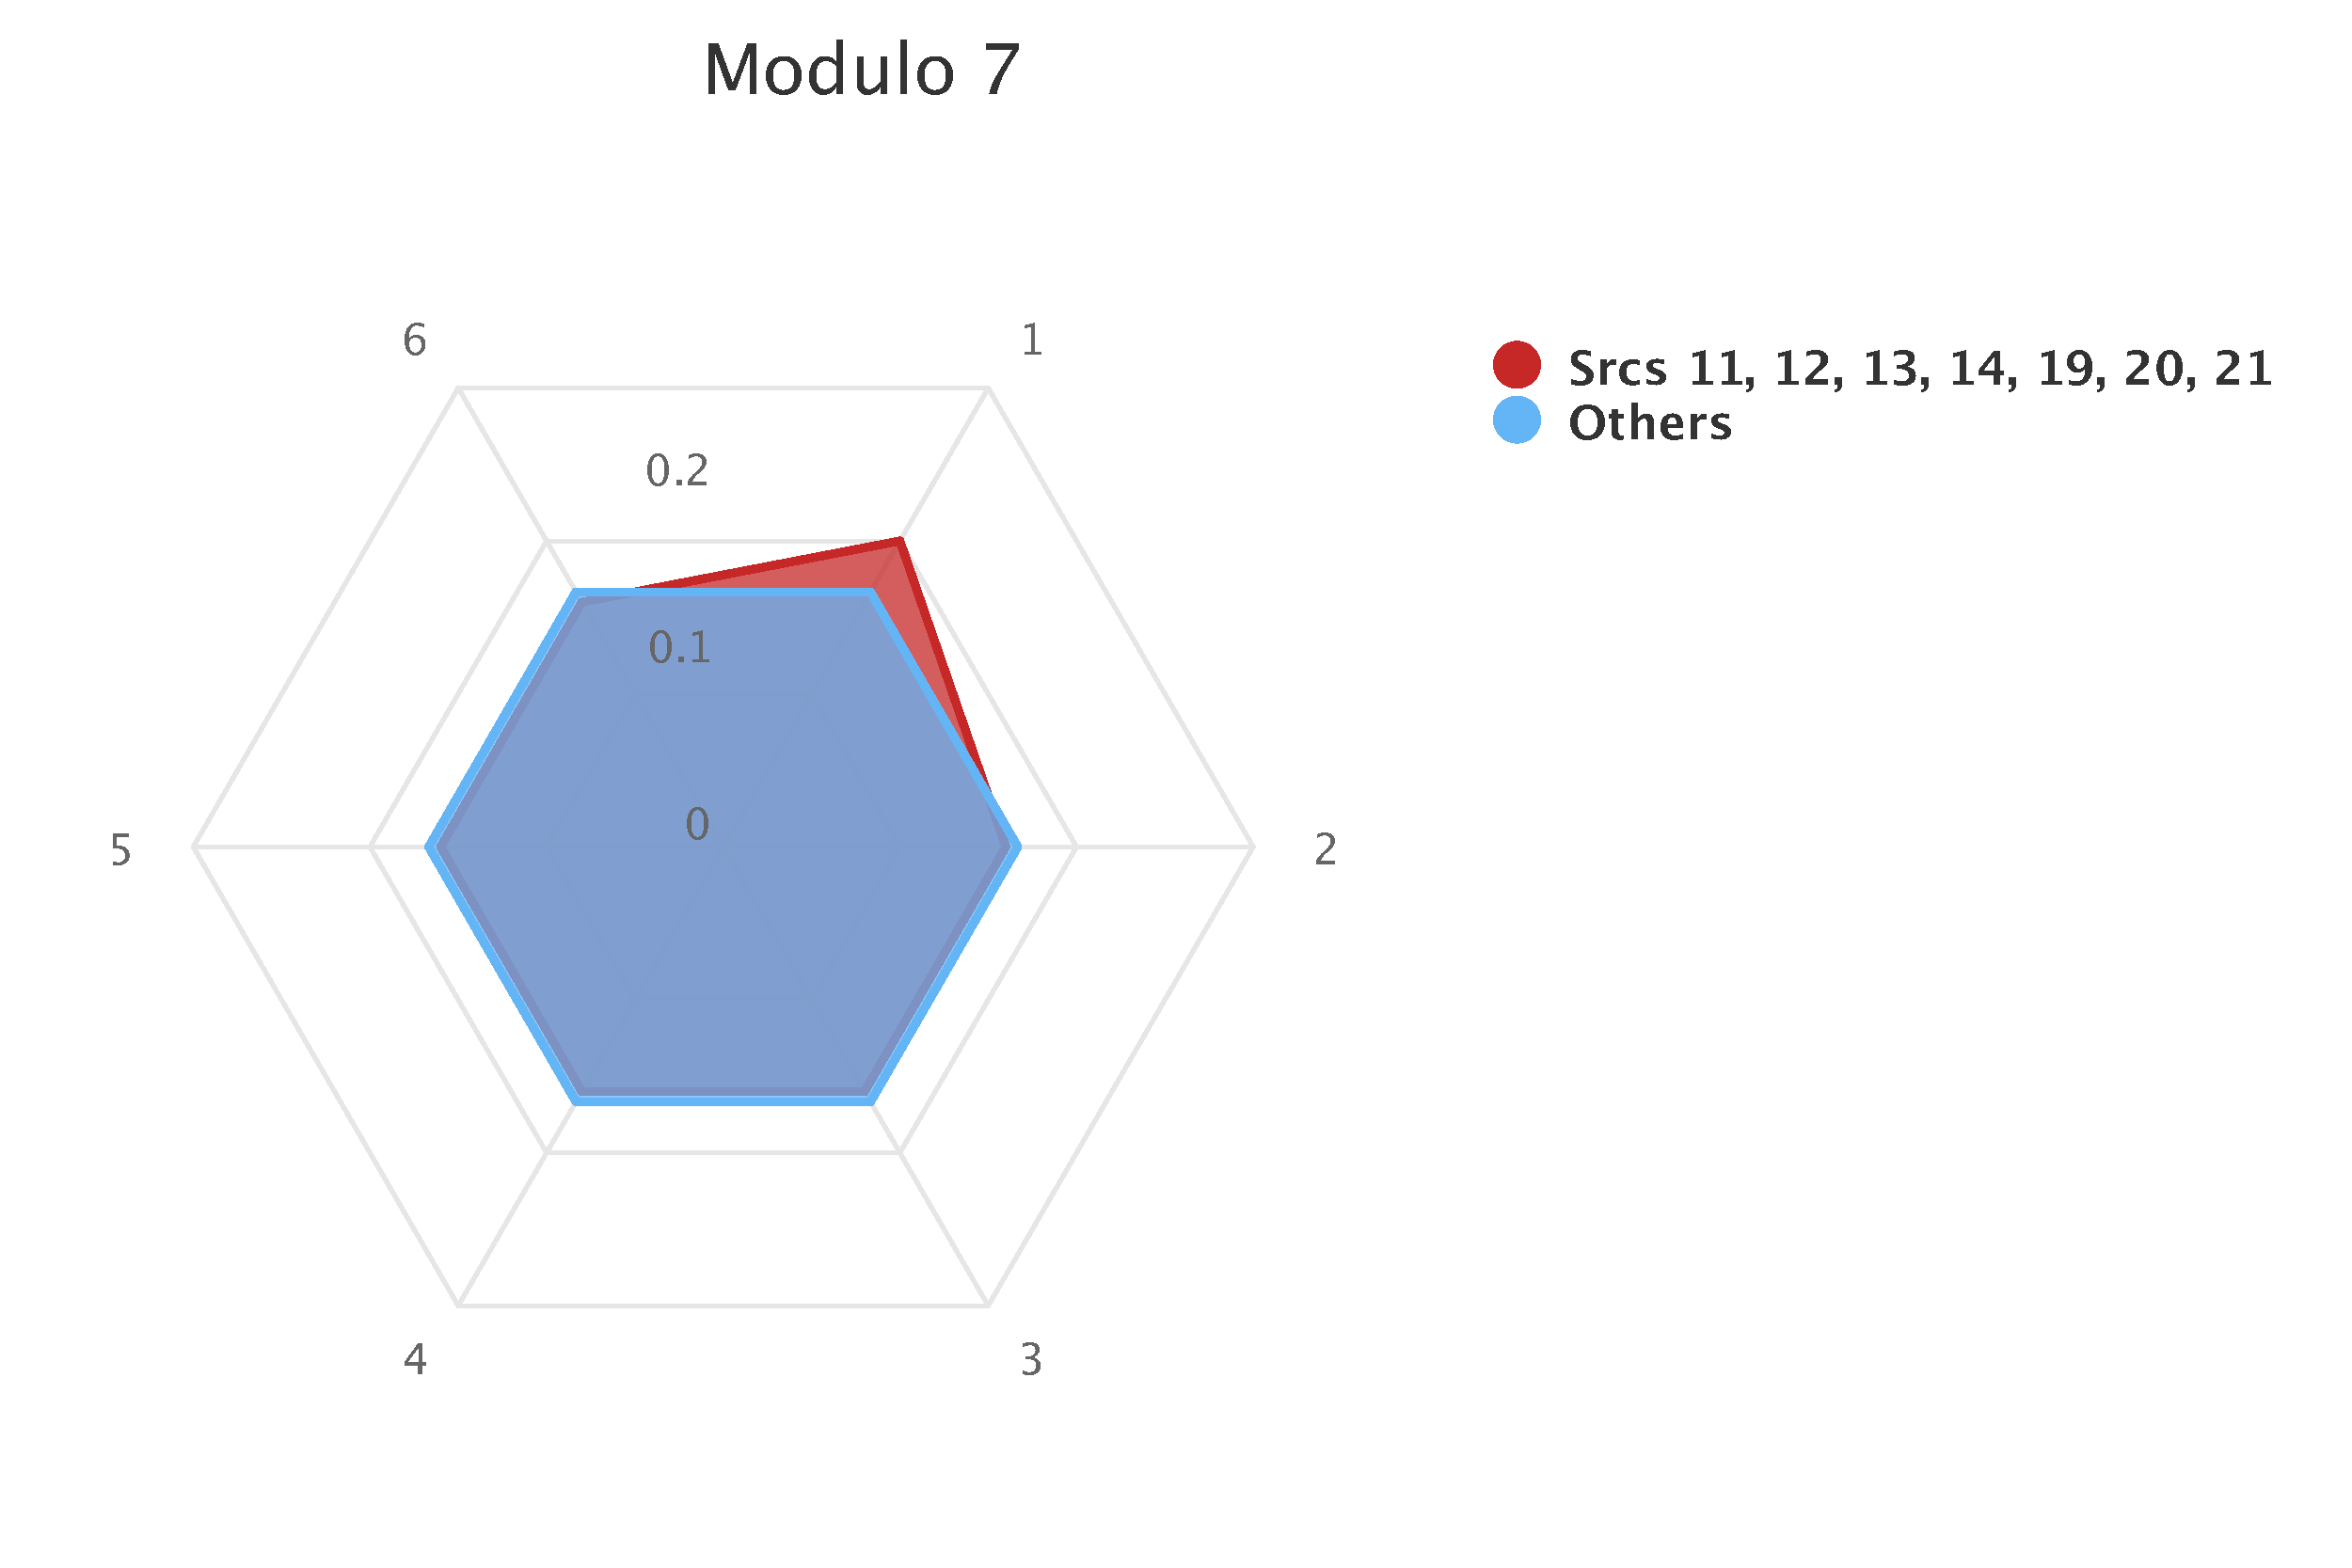
\includegraphics[width=\linewidth]{tex/images/analysis/mod7}
\end{subfigure}\\

\begin{subfigure}{0.45\textwidth}
	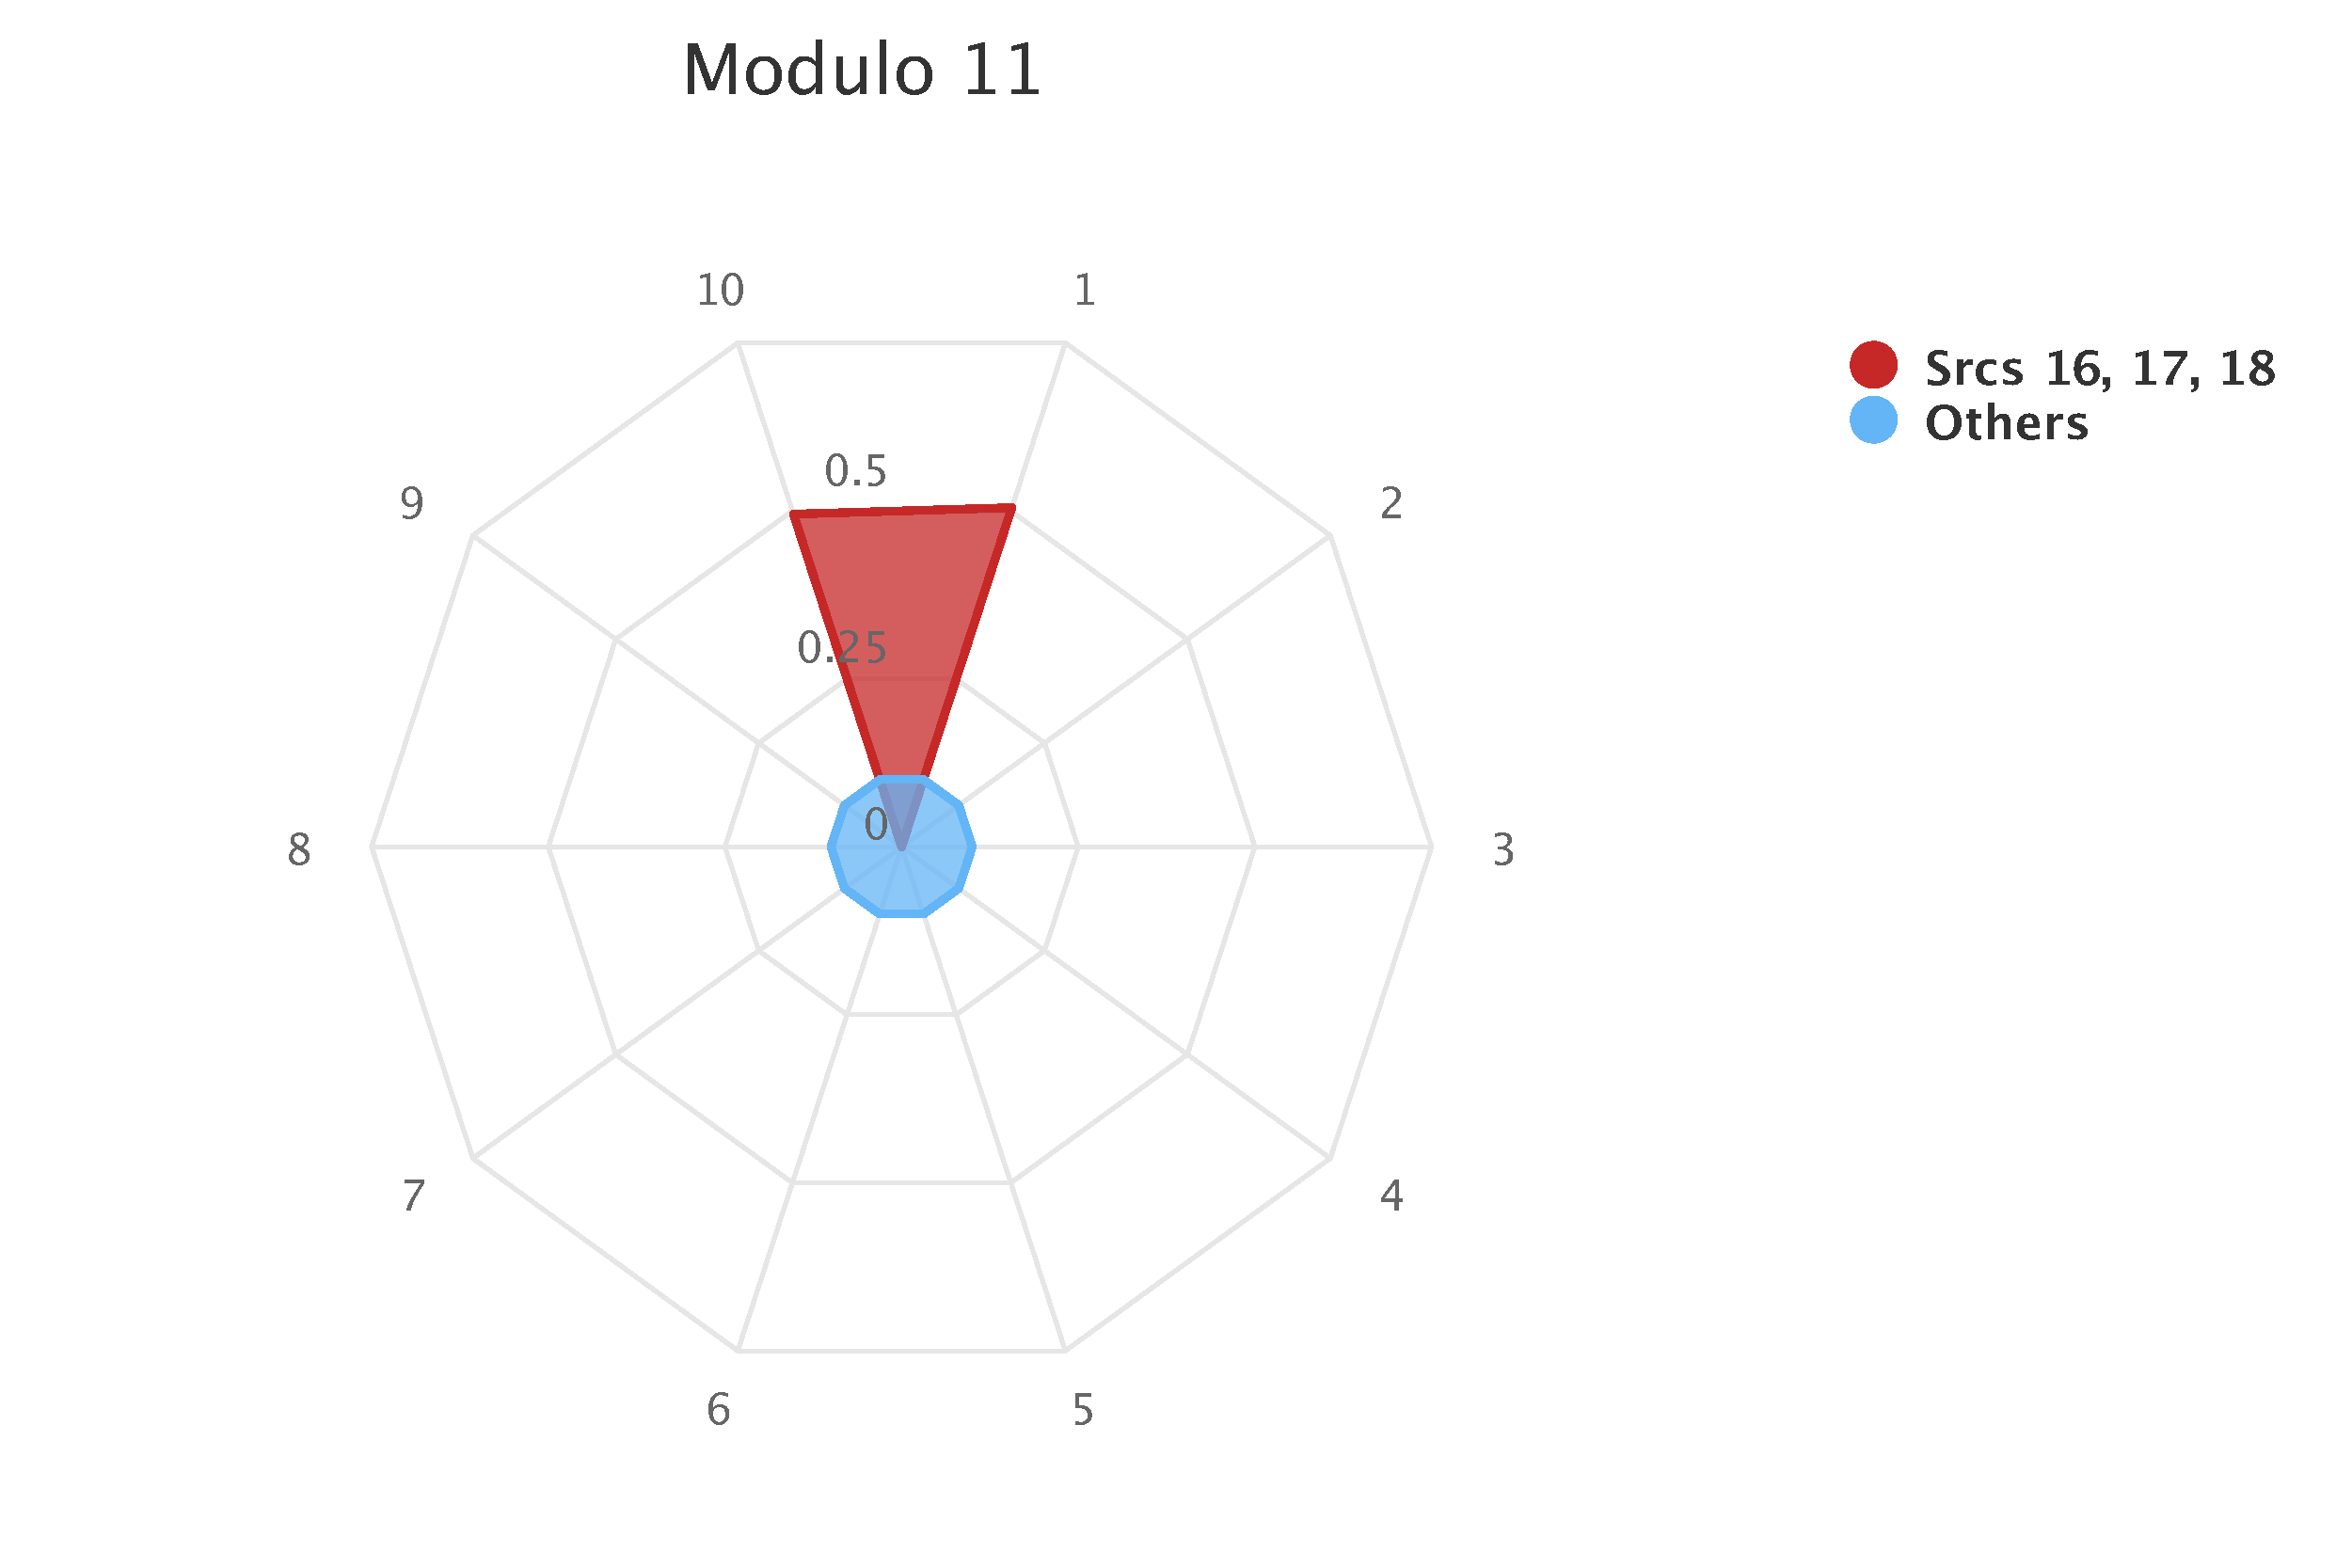
\includegraphics[width=\linewidth]{tex/images/analysis/mod11}
\end{subfigure}
\hfill
\begin{subfigure}{0.45\textwidth}
	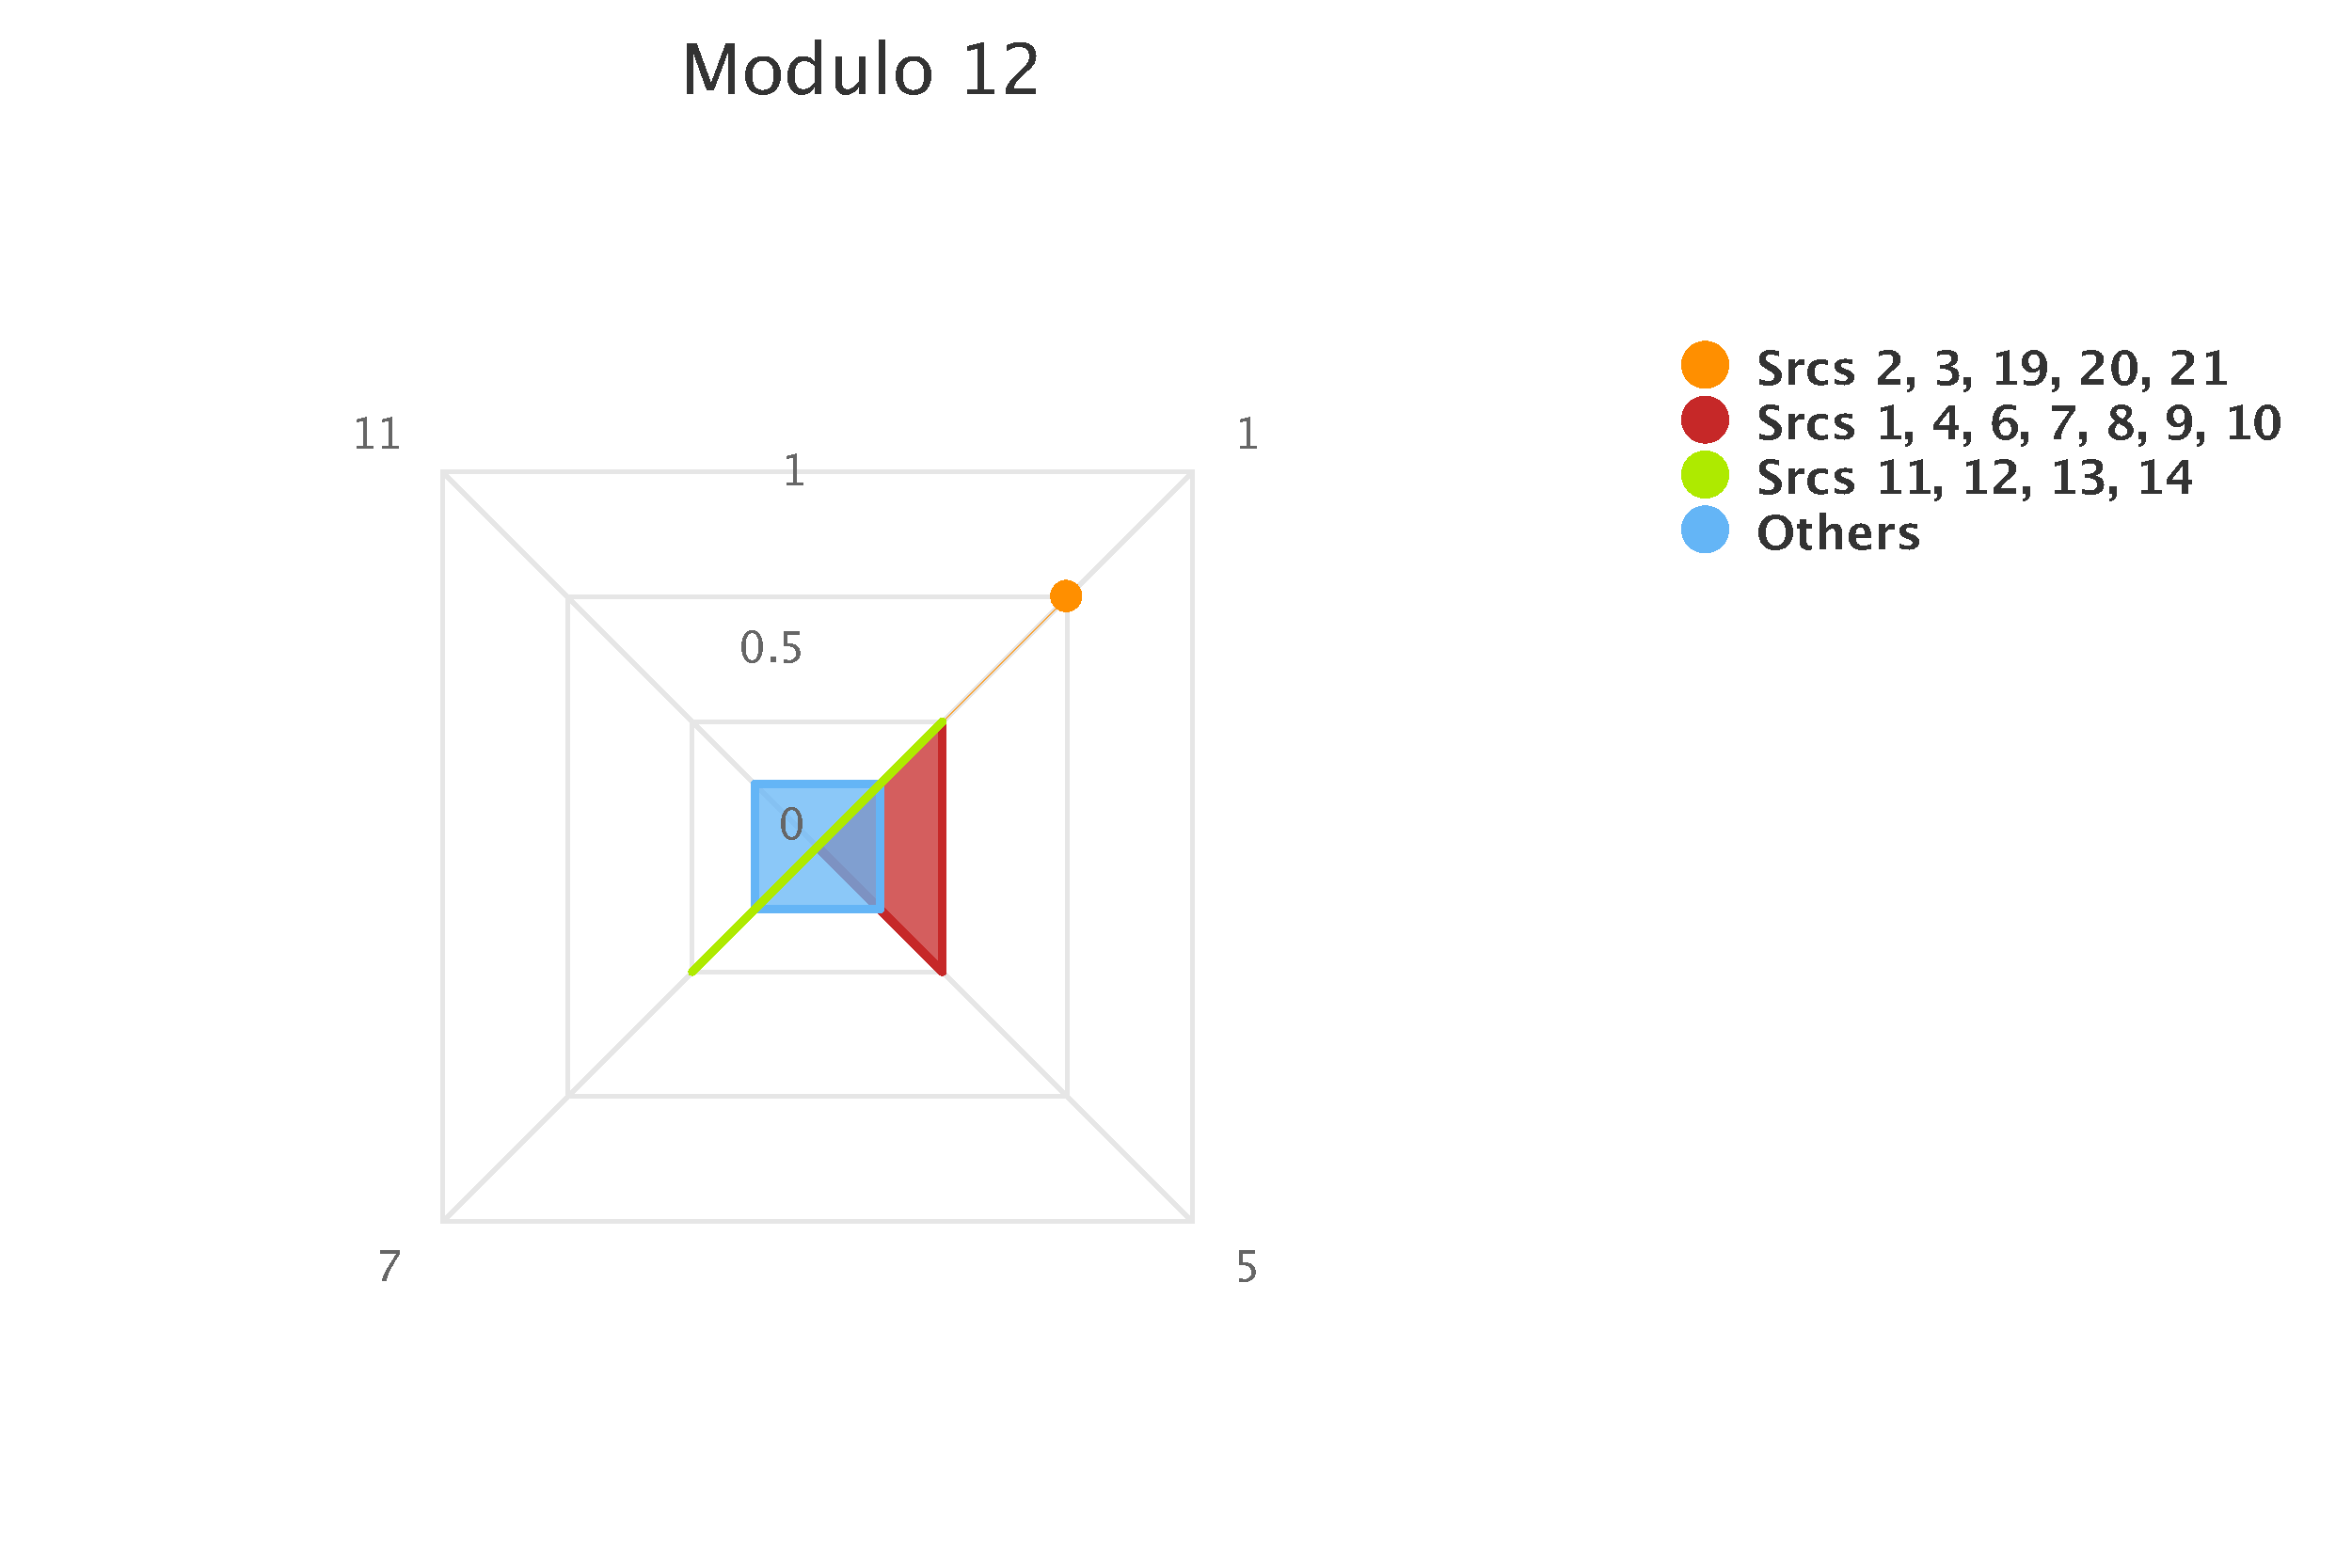
\includegraphics[width=\linewidth]{tex/images/analysis/mod12}
\end{subfigure}\\

\begin{subfigure}{0.45\textwidth}
	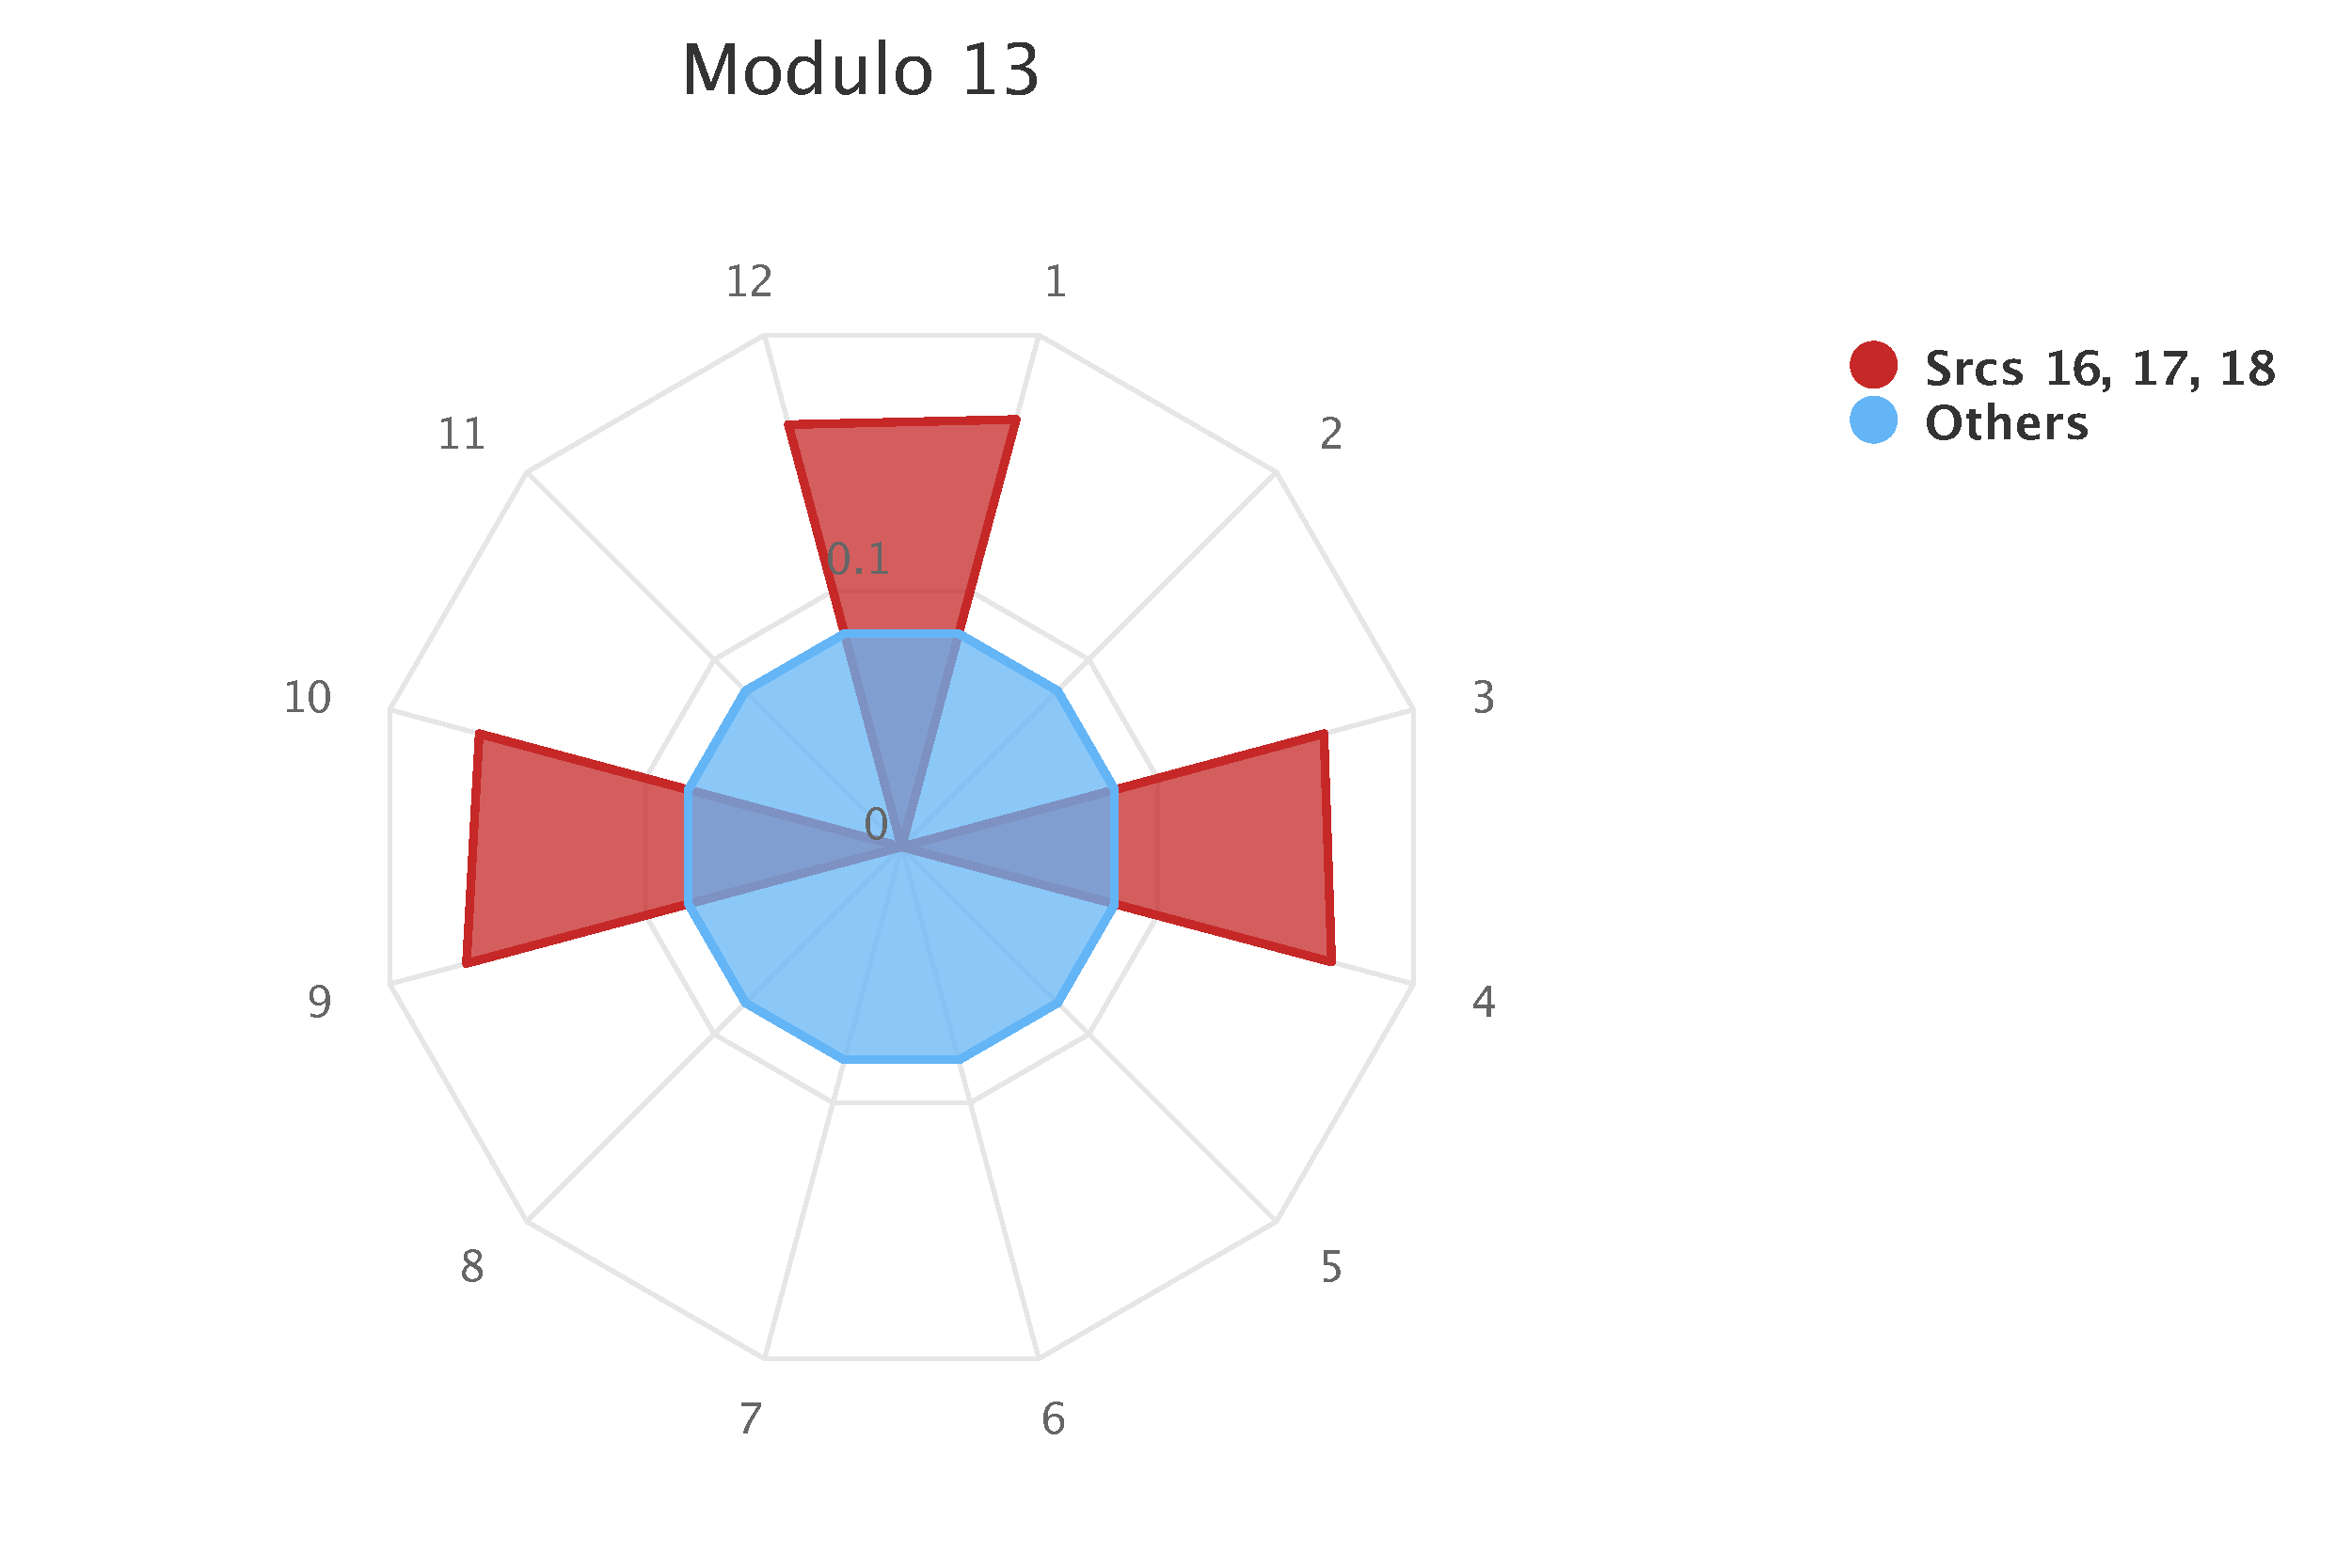
\includegraphics[width=\linewidth]{tex/images/analysis/mod13}
\end{subfigure}
\hfill
\begin{subfigure}{0.45\textwidth}
	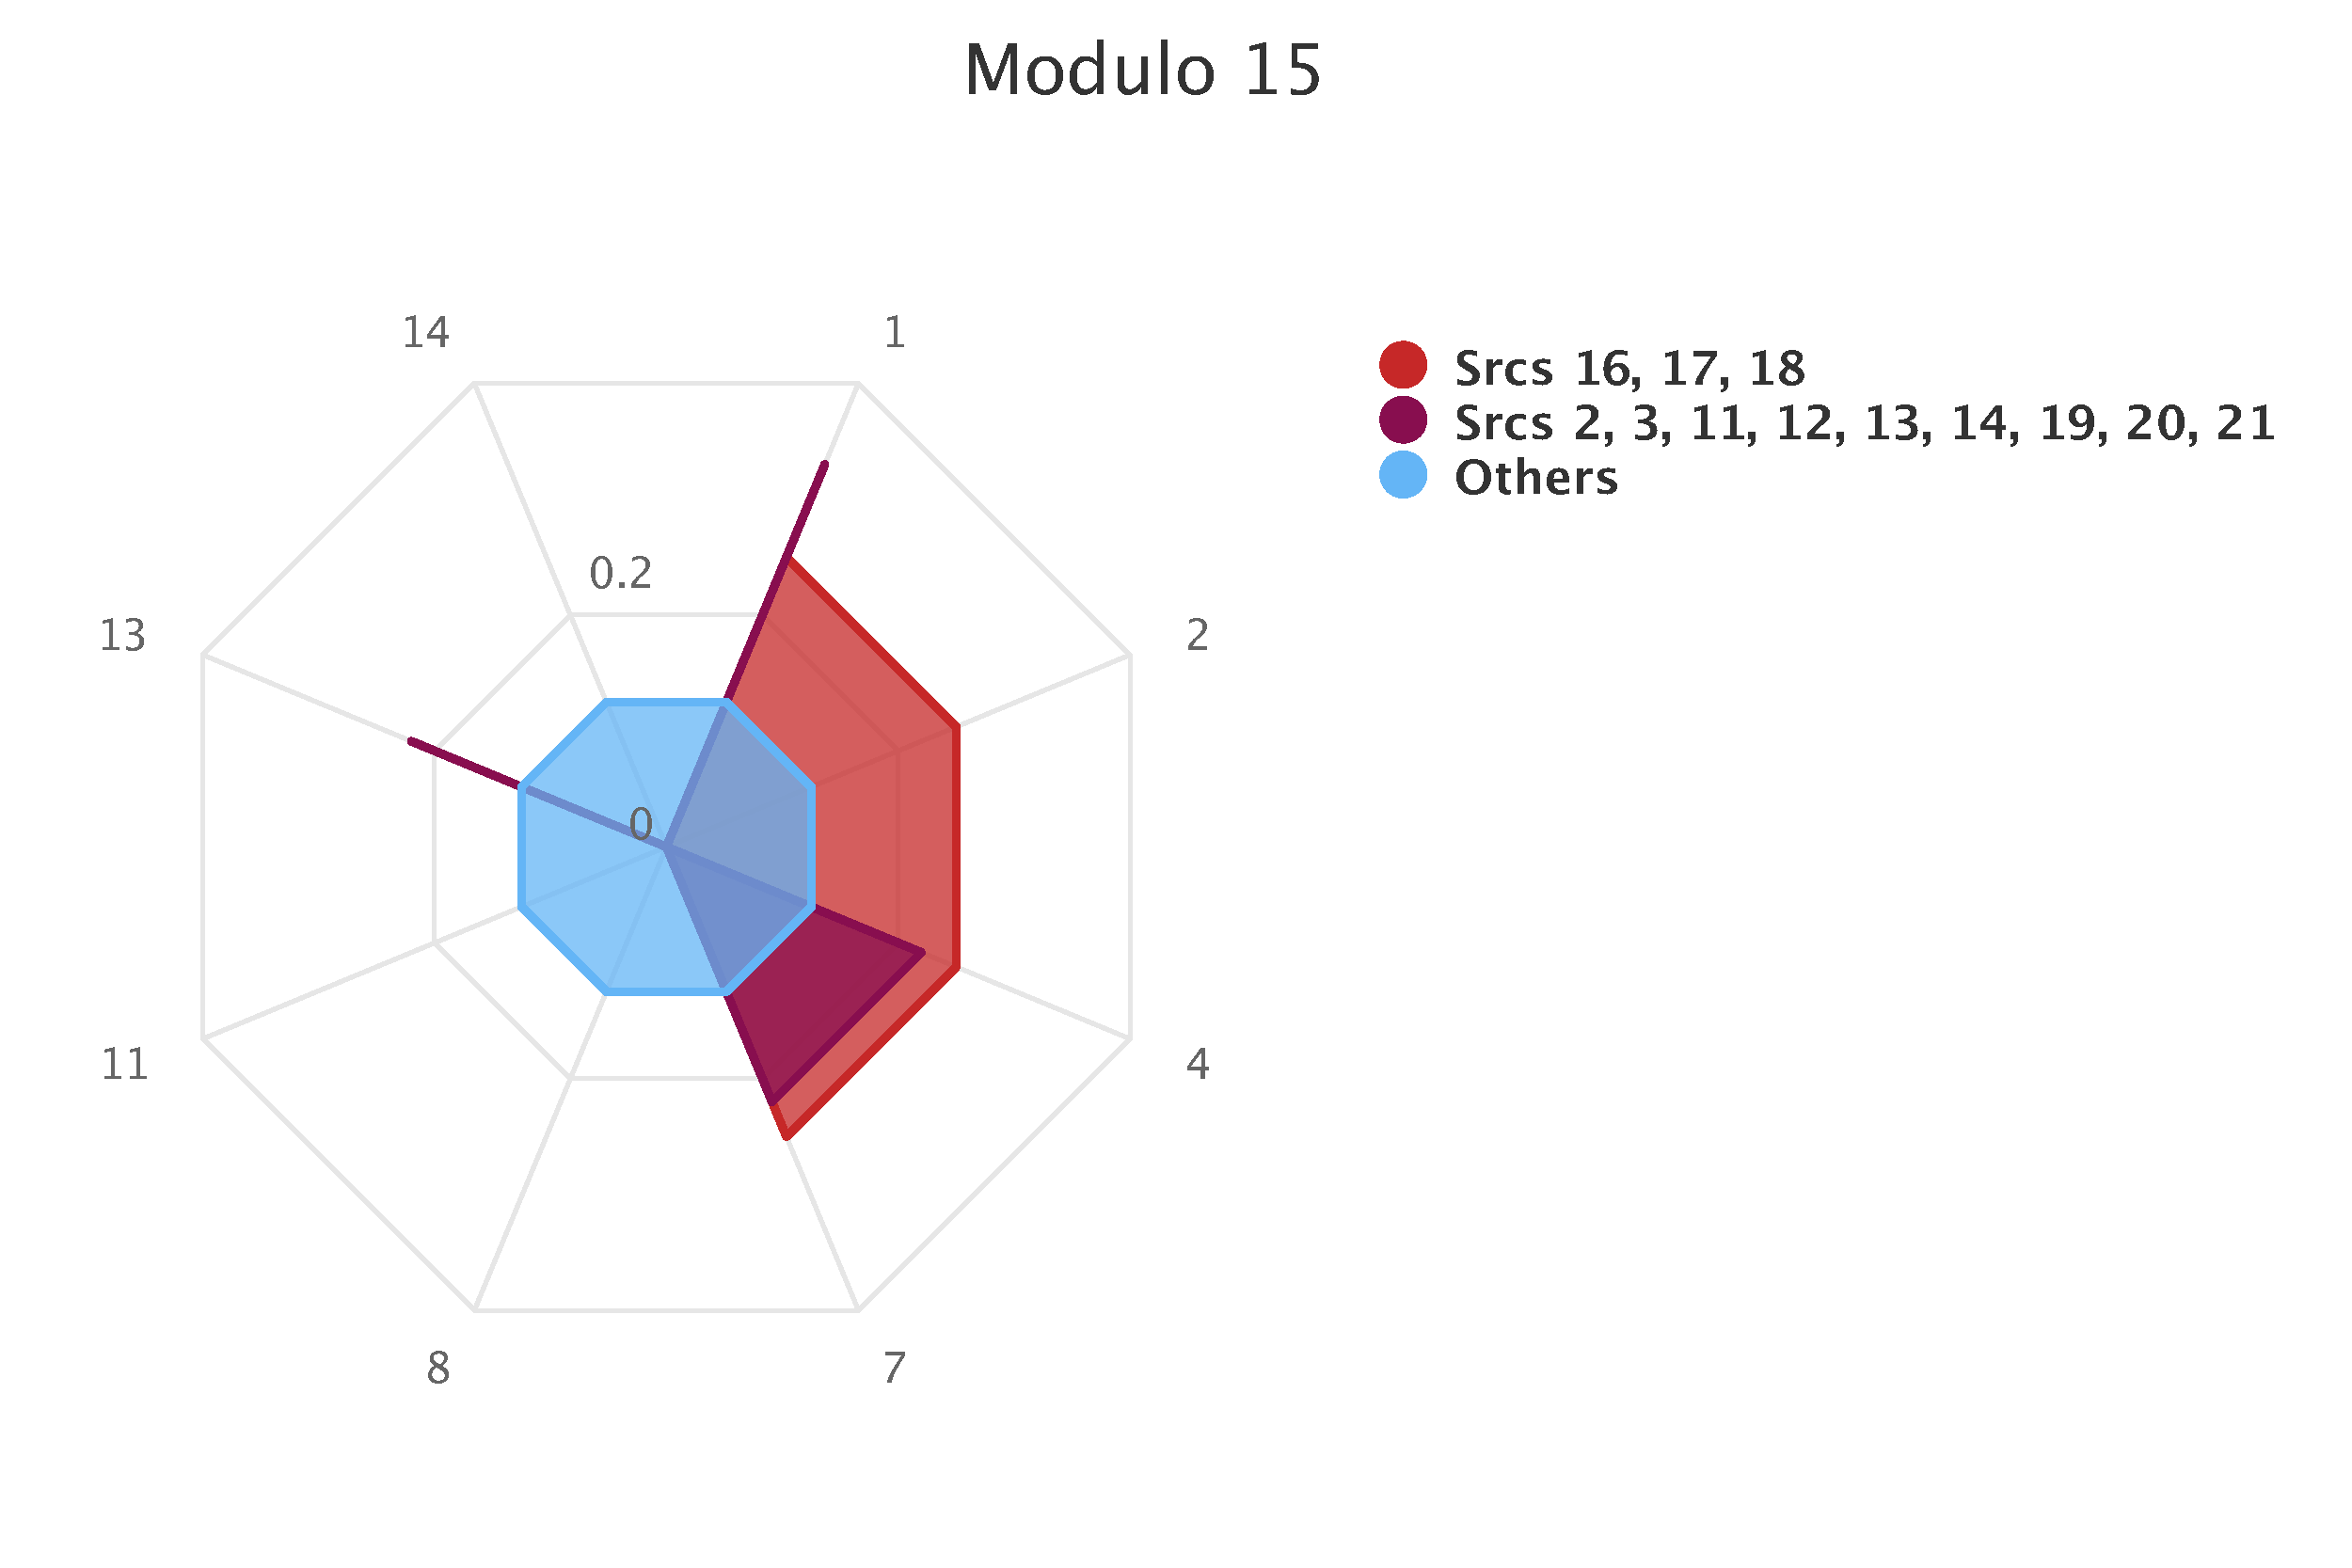
\includegraphics[width=\linewidth]{tex/images/analysis/mod15}
\end{subfigure}\\

\caption{Modular bias visualization, the following radar charts show the individual possible remainders. The blue area represents the uniform distribution, which includes most of the sources. The other colors are non-uniform distributions found in some sources. For example, sources 11-14, 19, 20, 21 are slightly biased towards 1 modulo 7.}
\end{adjustbox}
\end{figure}
\label{figure-mod-analysis}

\begin{figure}[ht]
\centering
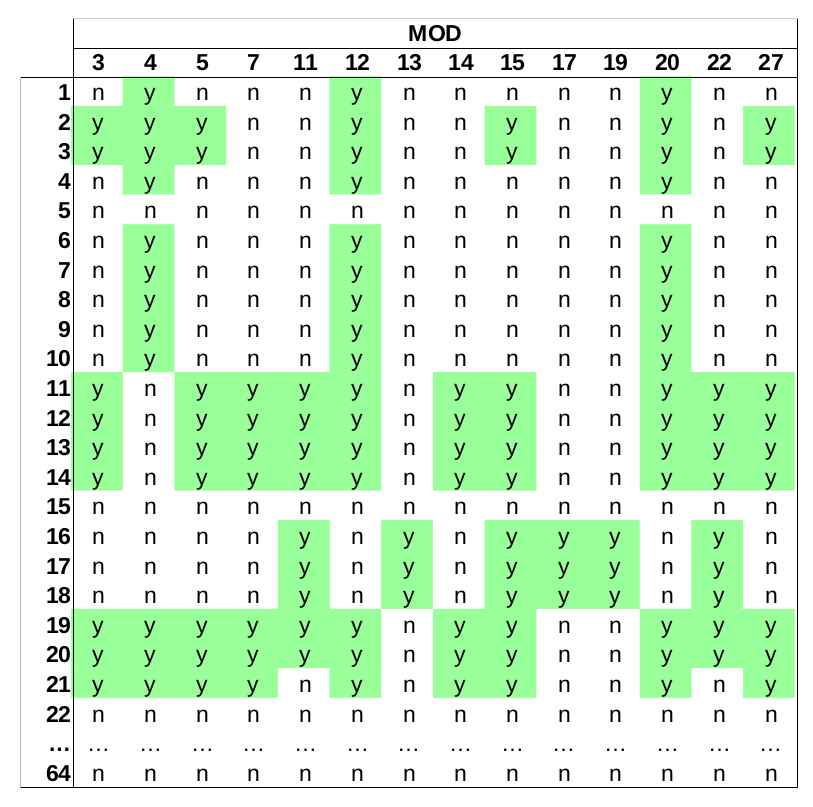
\includegraphics[width=0.64\textwidth]{tex/images/mod_analysis}
\caption{Table of biases. For sources 5, 15, 22-64 no biases have been found.}
\vspace{4in}

\end{figure}

\clearpage

\section{Bit analysis}
\label{appendix-bit-analysis}

\begin{figure}[ht]
	\centering
	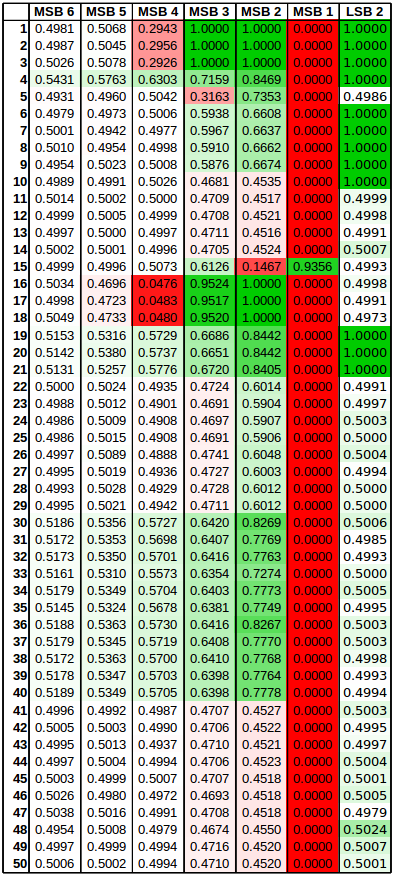
\includegraphics[width=0.47\linewidth]{tex/images/analysis/bit_sheet_1}
\end{figure}

\begin{figure}[ht]
	\centering
	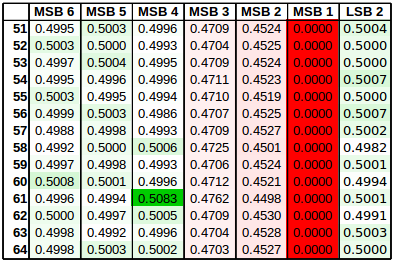
\includegraphics[width=0.47\linewidth]{tex/images/analysis/bit_sheet_2}
	\caption{Table of bit biases. The number represents the probability of 0 for a randomly chosen key.}
	\label{figure-table-bit-analysis}
\end{figure}

\begin{figure}[ht]
	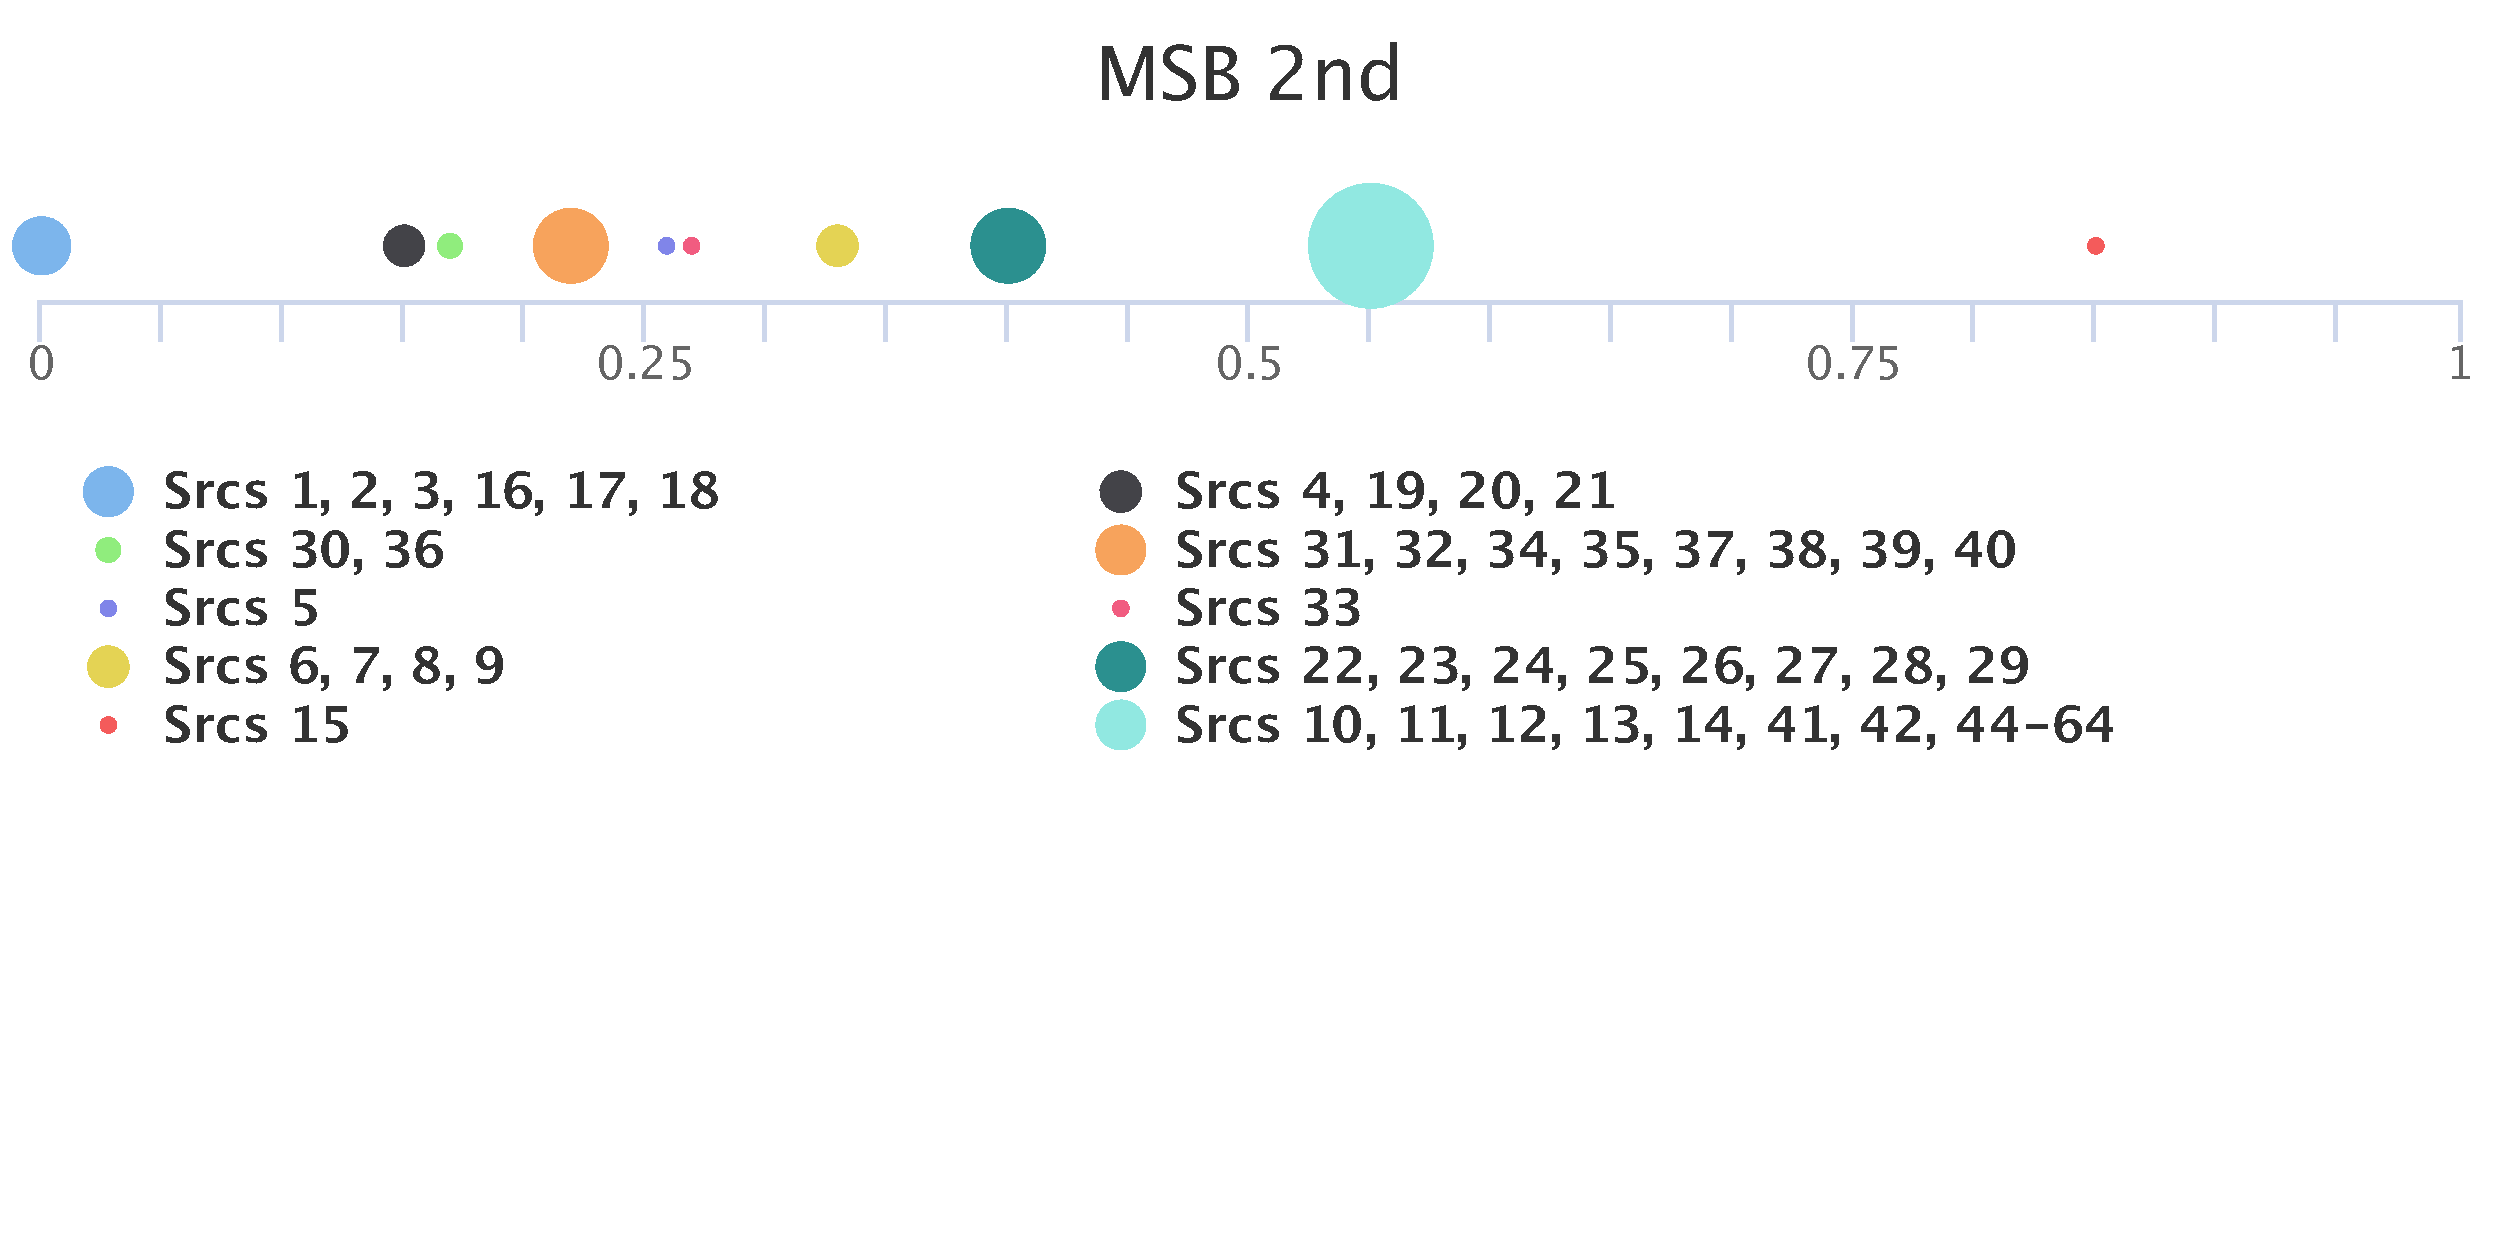
\includegraphics[width=\linewidth]{tex/images/analysis/bit2}
	\caption{Probability of 0 of 2nd most significant bit.}
\end{figure}

\begin{figure}[ht]
	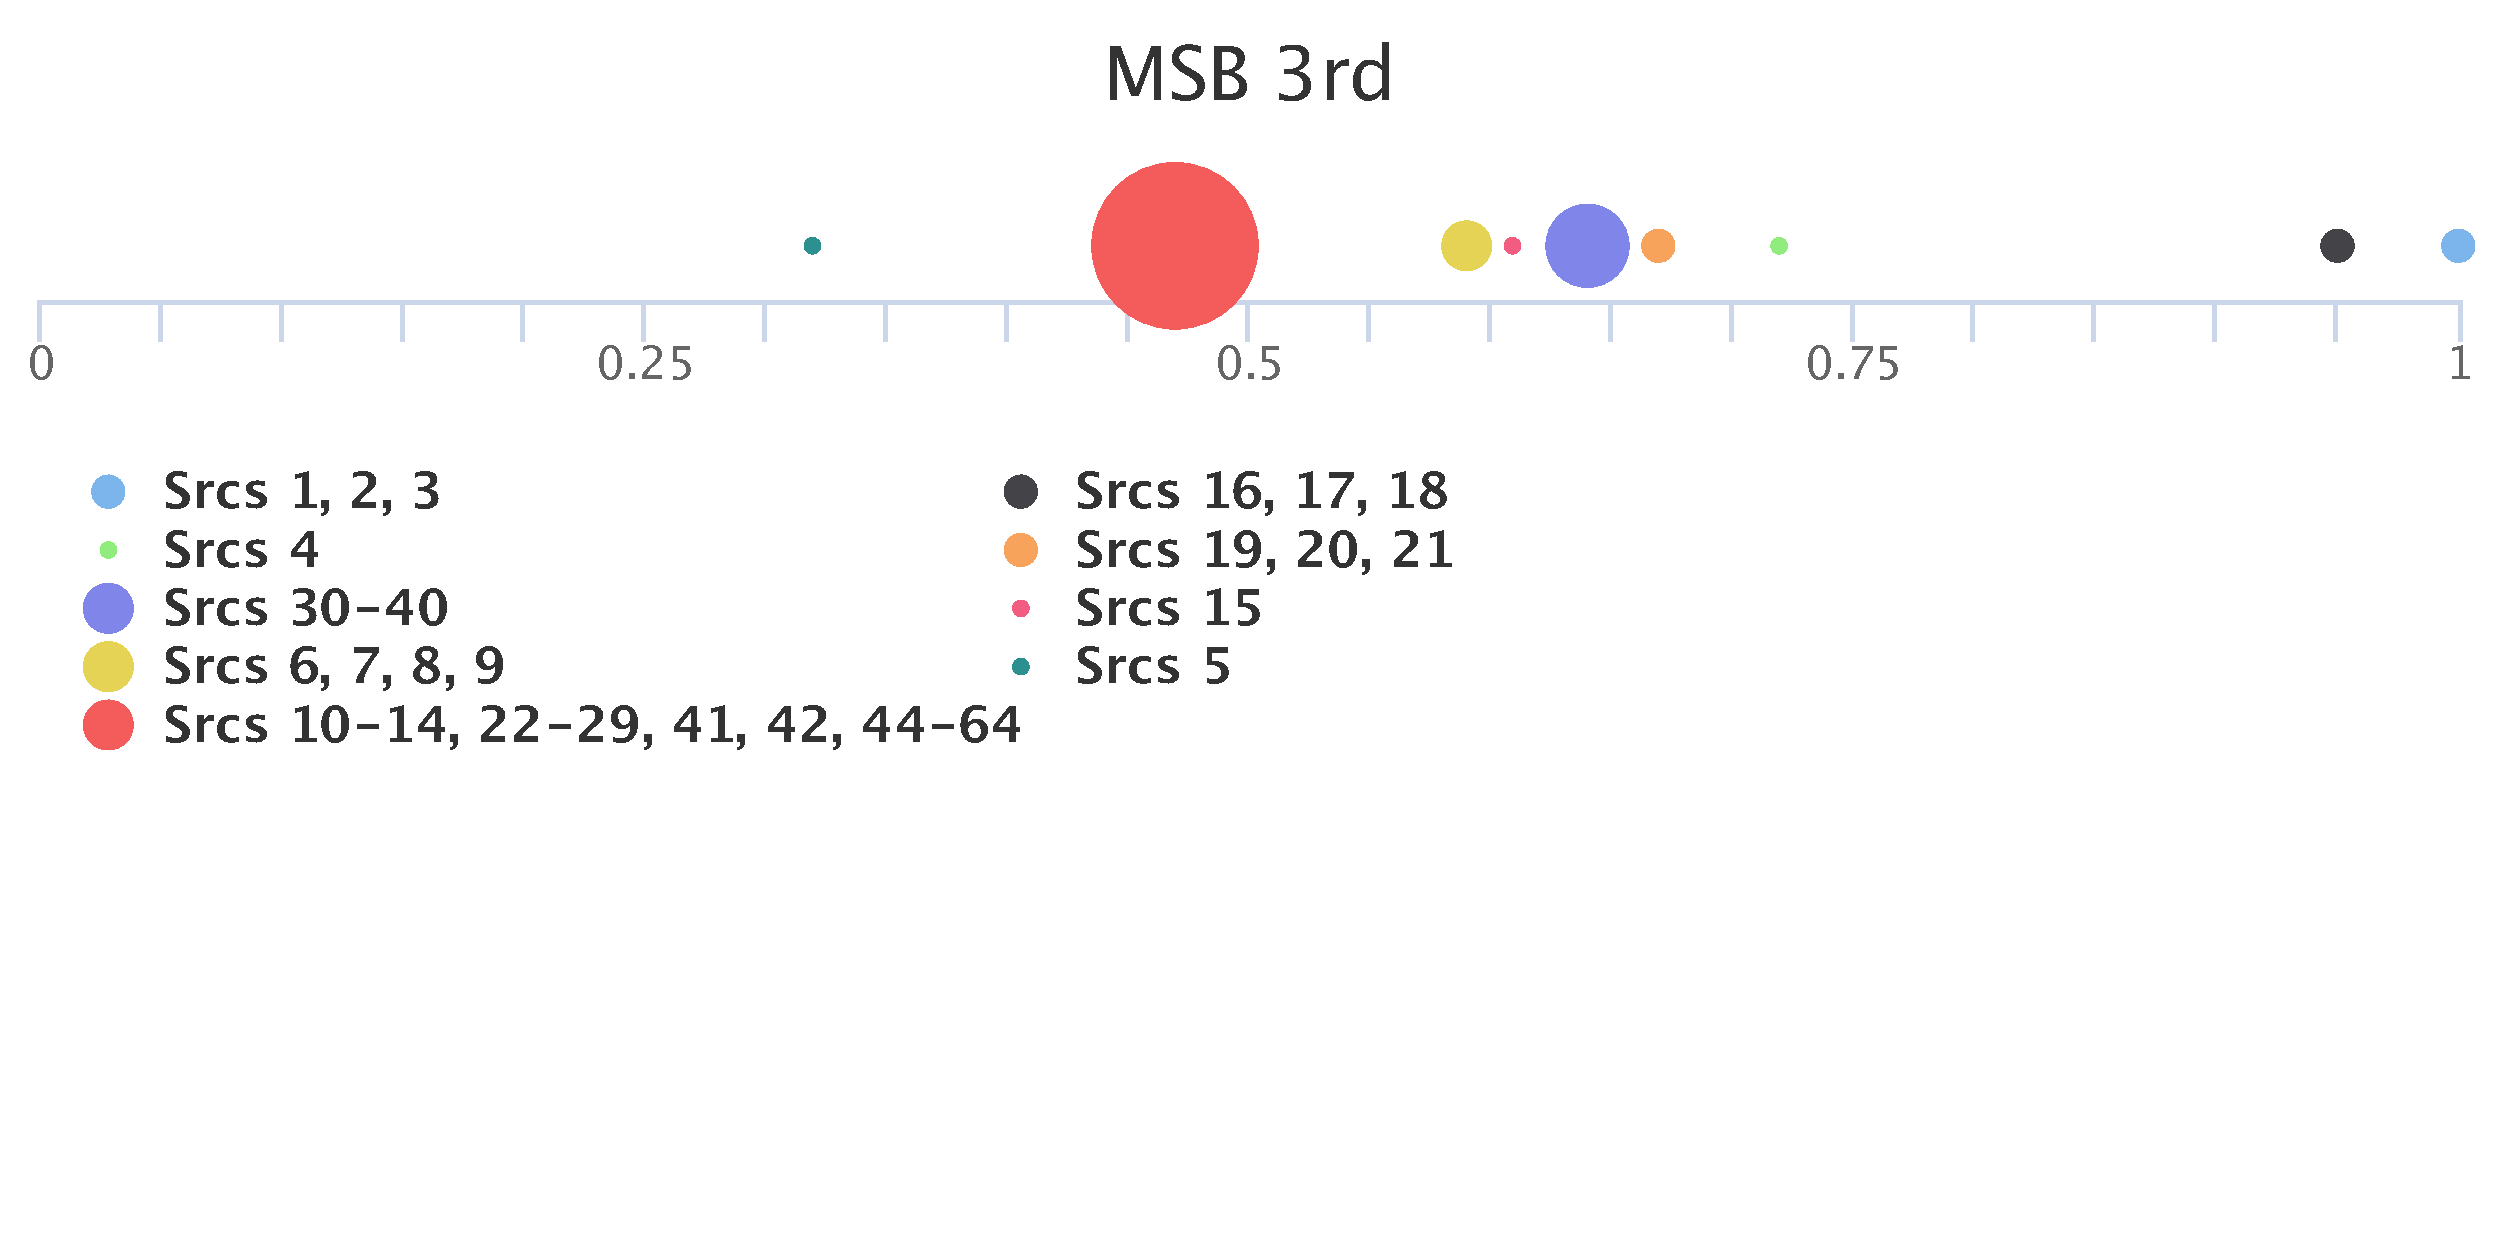
\includegraphics[width=\linewidth]{tex/images/analysis/bit3}
	\caption{Probability of 0 of 3rd most significant bit.}
\end{figure}

\begin{figure}[ht]
	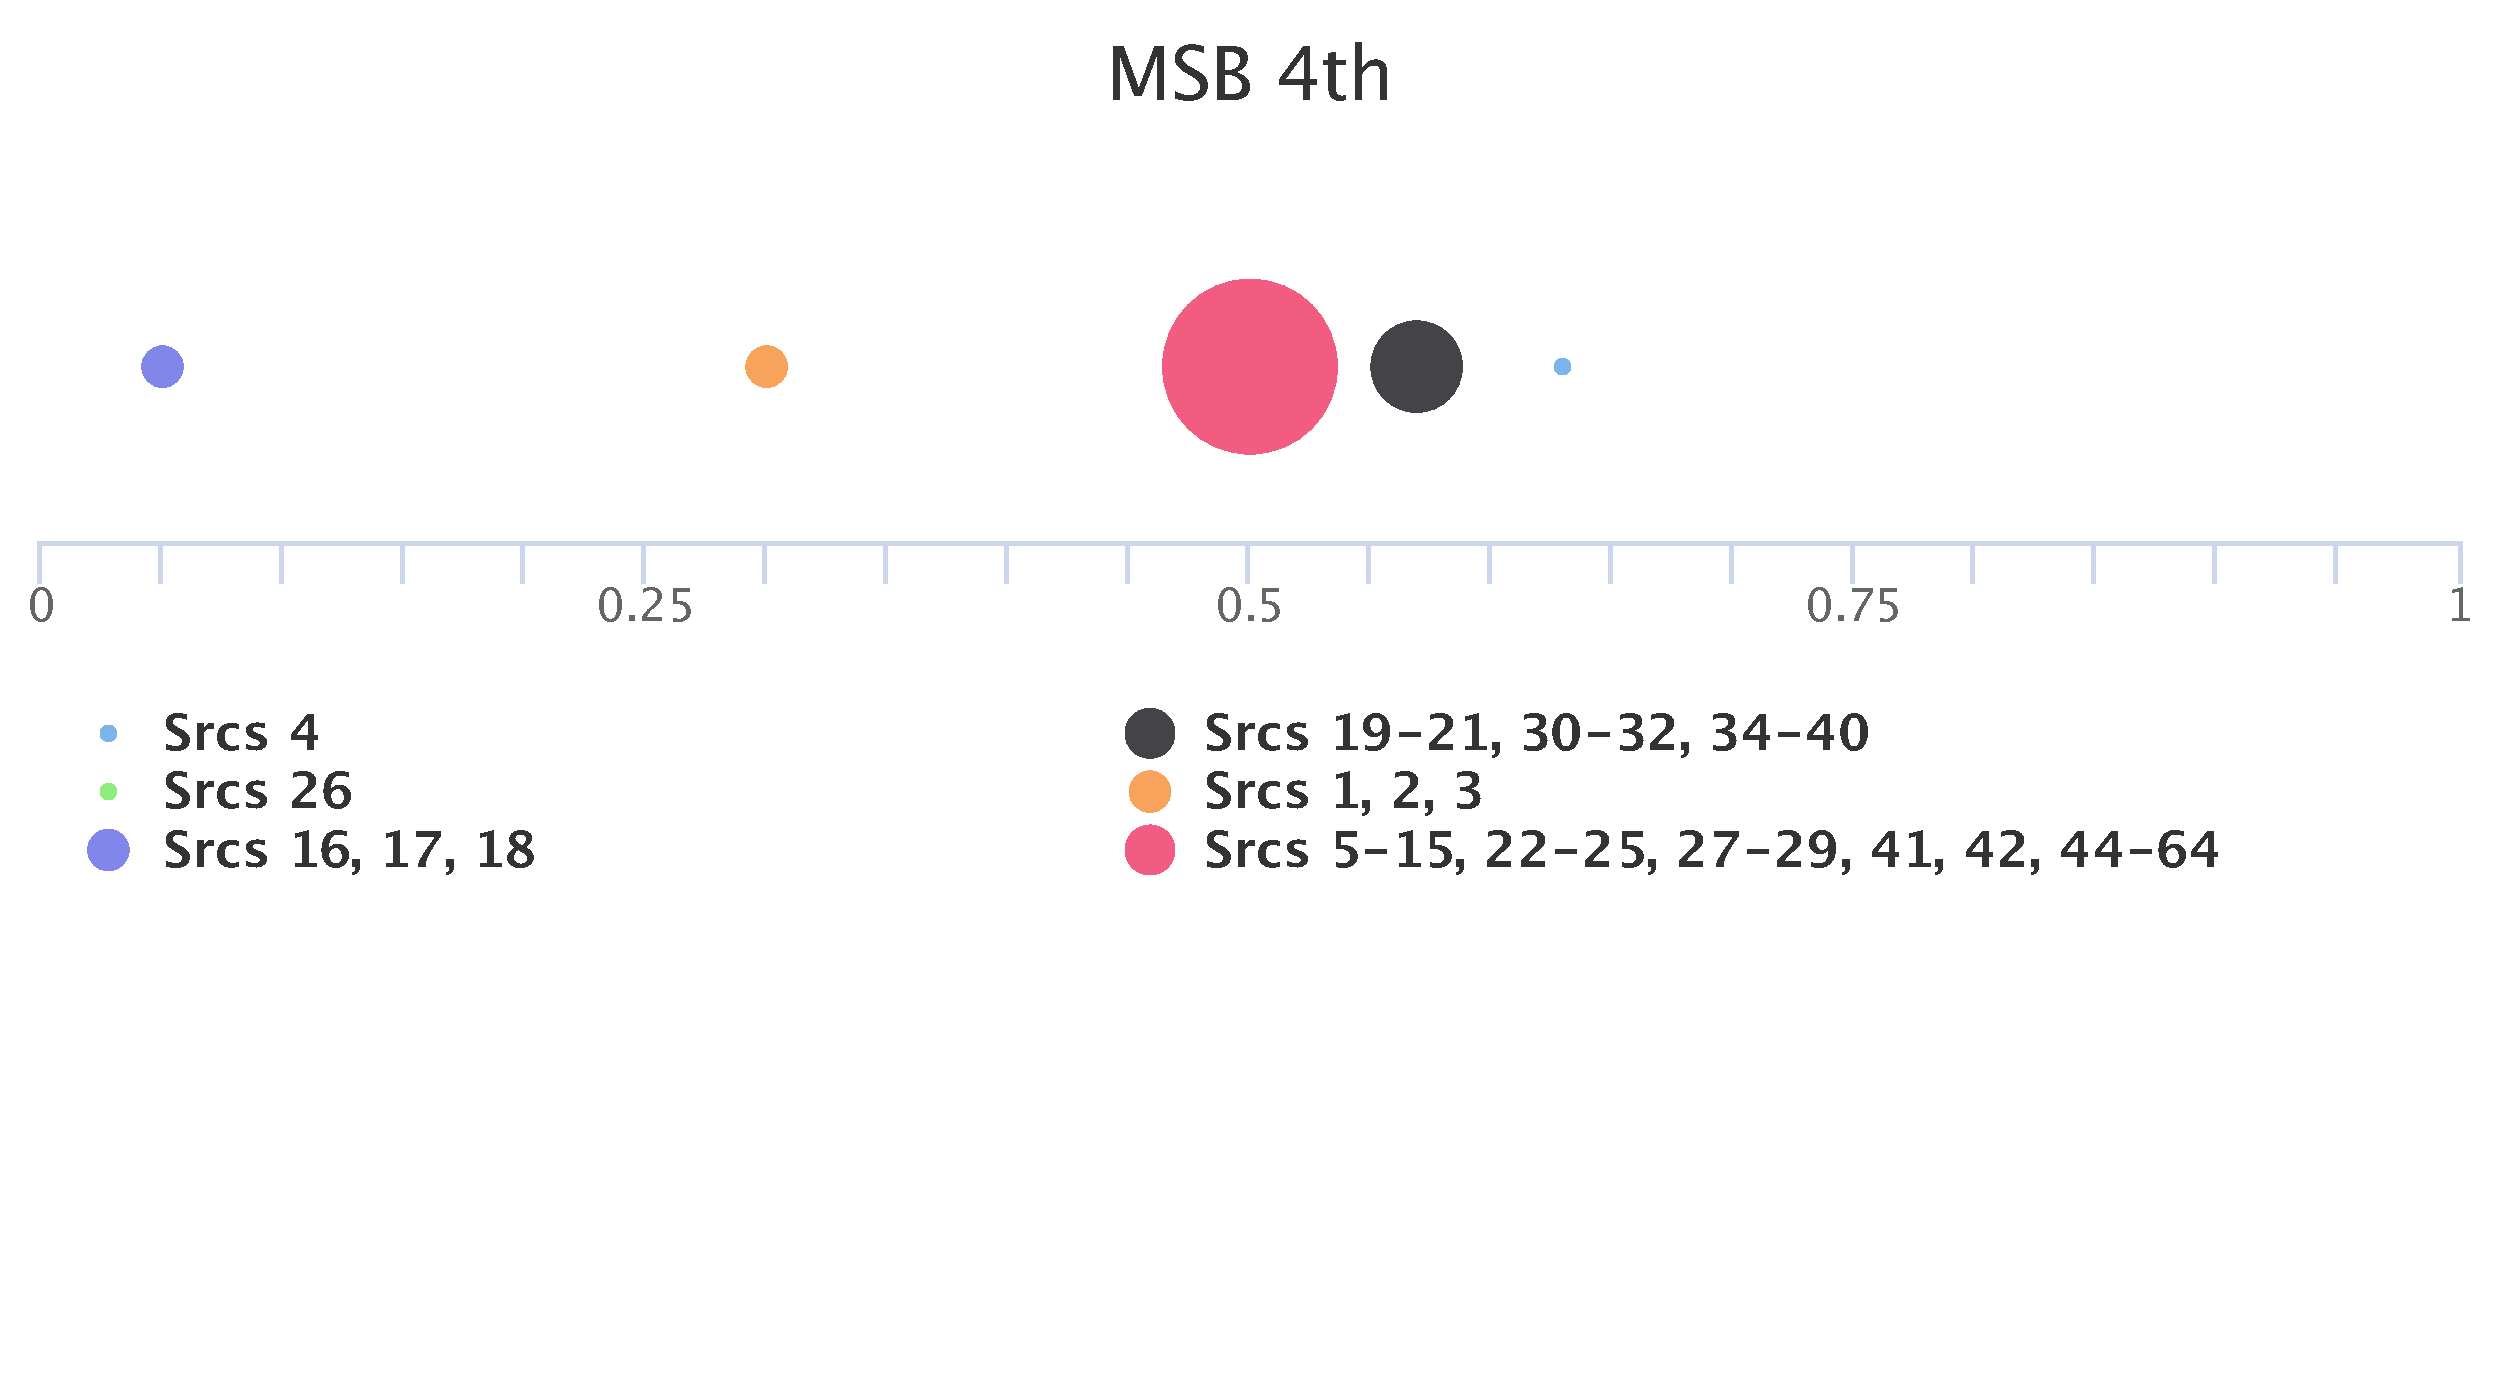
\includegraphics[width=\linewidth]{tex/images/analysis/bit4}
	\caption{Probability of 0 of 4th most significant bit.}
\end{figure}  
  \chapter{Application documentation and examples}

\label{appendix-running}

This appendix serves as simple documentation to the command line interface. 

\section{General settings}

The application is run via command \texttt{python3 cli.py [OPTIONS] TASK}\footnote{\textit{TASK} can be one of \textit{analyze, classify, generate, scan, train}}. The general options include:

\begin{itemize}

\item \texttt{--help} - Show help message an exit.
\item \texttt{--help-task TASK} - Show help message for specific task
\item \texttt{--settings PATH} - Path to custom yaml settings (if not specified, the default one is used)

\end{itemize}

\section{SCAN}

\noindent
Requires three arguments:

\begin{itemize}

\item \texttt{--scandir PATH} - directory to scan.
\item \texttt{--filter PATH} - path to filter JSON to apply.
\item \texttt{--output-json PATH} - path to the newly created sources JSON file.

\end{itemize}

\section{ANALYZE}

\noindent
Arguments:

\begin{itemize}

\item \texttt{--analyzed-csv PATH} - CSV file to analyze (required).
\item \texttt{--analysis-output PATH} - file to save analysis to. If not specified, then print to stdout.
\item \texttt{--json-format} - boolean flag, if true, then analysis is printed as JSON (used for further automatization).

\end{itemize}

\noindent
All arguments can be setup alternatively in YAML file. Further configuration in YAML include:

\begin{itemize}

\item \texttt{common.batch\_size} - chunk of data read in every iteration.
\item \texttt{common.keys\_per\_feature} - applies to FeatureMaker, should be set to 1 (usually, we analyze CSV files with each line representing only one key).
\item \texttt{fm.key\_length} - 512, 1024 or 2048
\item \texttt{fm.binary\_only} - whether or not the features should be represented by binary vectors only (for analysis should be setup to 0)
\item \texttt{fm.features} - features to analyze

\end{itemize}

\noindent
Supported features include\footnote{Features are described in \autoref{feature-maker}}:

\begin{itemize}

\item \texttt{['bit', \{'i': x\}]} (where \texttt{x} is bit index)
\item \texttt{['mod', \{'n': x\}]} (where \texttt{x} is divisor)
\item \texttt{'line'} (shortcut for taking every bit) 
\item \texttt{'mod3'} (shortcut for \texttt{['mod', \{ 'n': 3 \}]})
\item \texttt{'mod4'} (shortcut for mod 4)
\item \texttt{['xor', \{'indices': (x, y)\}]} (where \texttt{(x, y)} are bit pairs)

\end{itemize}

\subsection*{Example}

To run help about task:

\begin{minted}[ framesep=2mm,
                autogobble,
                frame=lines]{shell}

python3 cli.py analyze --help-task

\end{minted}

\noindent
The example below show the usage of the analyze task. First of all, setup YAML:

\begin{minted}[ framesep=2mm,
                autogobble,
                frame=lines]{yaml}

common:
  batch_size: 500000
  keys_per_feature: 1
...  
fm:
  key_length: 1024
  binary_only: 0
  features:
  - ['mod', {'n': 3}]
  - ['mod', {'n': 4}]
  - ['mod', {'n': 5}]

\end{minted}

\noindent
Then run command:

\begin{minted}[ framesep=2mm,
                autogobble,
                frame=lines]{shell}

cli.py analyze --analyzed-csv <PATH/TO/CSV> \
--analysis-output <PATH/TO/OUTPUT> \
--json-format

\end{minted}

\noindent
This will run the analyze task and on the \texttt{<PATH/TO/CSV>} file, that have 1 key per line of length 1024 bits in batches of 500000 lines. The analyzed features are moduli of 3, 4 and 5. The output is saved in \texttt{<PATH/TO/OUTPUT>} json file. The output can look like:

\begin{minted}[ framesep=2mm,
                autogobble,
                frame=lines]{json}

"feature_counter": {
  ...
  "2": {
    "('mod', 5)": {
      "[1]": 16821,
      "[2]": 11206,
      "[3]": 11006,
      "[4]": 10967      
    },
    "('mod', 4)": {
    ...  
  },
  ...
},
"group_counter": {
  ...
  "('mod', 5)": {
    "[1]": {
      "1": 23371,
      "2": 16821,
      ...
    },
    ...
  },
  ...
}  

\end{minted}

\noindent
Feature counter shows the counts for features per each group (\texttt{group.feature.value}). Here we can see, that group 2 has bias towards the remainder 1 when divided by 5. The group counter shows the counts for groups per each feature (\texttt{feature.value.group}). Here we can see, that even though the group 2 has bias towards 1 and group 1 is uniformly distributed modulo 5, there is higher chance of getting group 1 than 2. The result could mean, that the neural network would be biased towards the group 1, if this would be the training data.


\section{GENERATE}
\label{appendix-generate}

\noindent
Arguments:

\begin{itemize}

\item \texttt{--datapath PATH} - path to the generated dataset.
\item \texttt{--single/--dataset} - boolean flag to generate either single CSV or CSV triplet (by default triplet is generated).
\item \texttt{--shuffle/--no-shuffle} - boolean flag, if set, then the target dataset is shuffled (by default is true).
\item \texttt{--sources-path PATH} - sources JSON file generated by SCAN task.
\item \texttt{--relabel} - boolean flag, if set, then relabels the target sources to have consecutive integer numbers (starting with 1).  Can be useful when any groups are skipped, or some group is missing.

\end{itemize}

\noindent
YAML:

\begin{itemize}

\item \texttt{common.batch\_size} - same as with \textit{ANALYZE}.
\item \texttt{common.keys\_per\_feature} -  specifies how many keys should be put into one line of target CSV.
\item \texttt{common.valid\_ratio} - the percentage of validation data (a number between 0 and 1). Applicable only to \texttt{--dataset} option.
\item \texttt{common.test\_ratio} - the percentage of test data (a number between 0 and 1). Applicable only to \texttt{--dataset} option.
\item \texttt{common.number\_of\_groups} - number of groups of the source dataset.
\item \texttt{generate.keys\_per\_group} - how many keys are taken per each group (the generator automatically scales this number within its sources).
\item \texttt{generate.skipped\_groups} - which groups should not be included in the final dataset (i. e. \texttt{skipped\_groups: ["3", "8"]}).
\item \texttt{generate.skipped\_files} - which sources should not be included in the final dataset.
\item \texttt{generate.train\_keys\_multiplicity} - dictionary, where the key specifies the group and the value specifies the multiplicity ratio for train keys. Applicable only to \texttt{--dataset} option.
\item \texttt{generate.merge\_groups} - lists of merged groups (i.e. \texttt{[6,7,8,9]}  merges groups 6, 7, 8, 9 together).

\end{itemize}

\subsection*{Example}

To run help about task:

\begin{minted}[ framesep=2mm,
                autogobble,
                frame=lines]{shell}

python3 cli.py generate --help-task

\end{minted}

\noindent
The example below was used to generate a uniform dataset for 13 groups from our  modified dataset. YAML configuration:

\begin{minted}[ framesep=2mm,
                autogobble,
                frame=lines]{yaml}

common:
  batch_size: 1000000
  keys_per_feature: 1
  valid_ratio: 0.2
  test_ratio: 0.2
  number_of_groups: 64 # the original dataset has 64 sources
...  
generate:
  keys_per_group: 200000
  skipped_groups: []
  skipped_files: []
  train_keys_multiplicity: # replicate training data in small sources
    1: 2
    2: 2
    5: 4
    17: 2
    18: 3
    21: 5
  merge_groups: # merge sources in the same group
  - [2,3]
  - [6,7,8,9]
  - [11,12,13,14]
  - [16,17,18]
  - [19,20,21]
  - [22,23,24,25,26,27,28,29]
  - [30,31,32,33,34,35,36,37,38,39,40]
  - [41,42,43,44,45,46,47,48,49,50,51,52,53,54,55,56,57,58,59,60,61,62,63,64]
\end{minted}

\noindent
To generate the new dataset we used the JSON file for 1024 bit sources with command:

\begin{minted}[ framesep=2mm,
                autogobble,
                frame=lines]{shell}

cli.py generate --sources-path sources/grouped_1024.json --dataset \
--datapath <PATH_TO_NEW_DATASET> --shuffle --relabel 

\end{minted}

\section{TRAIN}

\noindent
Arguments:

\begin{itemize}

\item \texttt{--datapath PATH} - same as with \textit{GENERATE}.
\item \texttt{--single/--dataset} - same as with \textit{GENERATE}.
\item \texttt{--incremental/--no-incremental} - boolean flag, with the incremental approach, python generators are used to fetch the data to the model, else the whole data is loaded into the memory (by default incremental).
\item \texttt{--results-to-file/--results-to-stdout} - print the train information to the result directory or stdout (by default directory is chosen).
\item \texttt{--model} - name of the used clWe designed a simple CLI for our application for the user. Can be specified in YAML as well.

\end{itemize}

Models are loaded from the models.json file. Key represents the name of the model passed to CLI. The base class is provided to load model dynamically. Further information is provided, which are necessary for a model interface for the specific library (for keras we specified name and topology). Example from this JSON file was shown in the description of the \textit{TRAIN} task in \autoref{models-json}.

Further configuration is set via YAML file:

\begin{itemize}

\item \texttt{common.batch\_size} - same as with \textit{ANALYZE}.
\item \texttt{common.keys\_per\_feature} - same as with \textit{GENERATE}. Specifies how many keys are present in one line of the CSV.
\item \texttt{common.valid\_ratio} - the percentage of validation data (a number between 0 and 1). Applicable only to \texttt{--single} option.
\item \texttt{common.test\_ratio} - the percentage of test data (a number between 0 and 1). Applicable only to \texttt{--single} option.
\item \texttt{common.number\_of\_groups} - same as with \textit{GENERATE}.
\item \texttt{train.epochs} - number of train epochs (applies to keras models).
\item \texttt{train.model} - name of the used model (CLI argument is prioritized).
\item \texttt{fm.*} - for all the settings for feature maker  apply the same description as with ANALYZE, but \texttt{fm.binary\_only} should be in this case 1 instead of 0 (binary vectors for modulo features are better for classifiers).

\end{itemize}

\subsection*{Example}

To run help about task:

\begin{minted}[ framesep=2mm,
                autogobble,
                frame=lines]{shell}

python3 cli.py train --help-task

\end{minted}

\noindent
The following example shows configuration from our train runs. YAML:

\begin{minted}[ framesep=2mm,
                autogobble,
                frame=lines]{yaml}

common:
  batch_size: 2048
  keys_per_feature: 1
  valid_ratio: 0.2
  test_ratio: 0.2
  number_of_groups: 13 # newly generated 13 sources
...  
train:
  epochs: 4
fm:
  key_length: 1024
  binary_only: 1
  features:
  - 'line'
  - 'mod3'
  - 'mod4'
  - ['mod', {'n': 5}]
  - ...
\end{minted}

\noindent
Command:

\begin{minted}[ framesep=2mm,
                autogobble,
                frame=lines]{shell}

python3 cli.py train --dataset --incremental \
--datapath <PATH_TO_NEW_DATASET> \
--model Keras28

\end{minted}

\noindent
Model topology configuration:

\begin{minted}[ framesep=2mm,
                autogobble,
                frame=lines]{json}

"Keras28": {"base": "KerasDeepClassifier",
             "name": "Keras ReLU Deep NN",
             "topology": {"hidden_layers": [{"activation": "relu",
                                             "number_of_neurons": 128},
                                            {"activation": "relu",
                                             "number_of_neurons": 1024}],
                          "loss": "categorical_crossentropy",
                          "metrics": ["acc"],
                          "optimizer": "Adadelta",
                          "output_layer": {"activation": "softmax"}}},

\end{minted}

The results are saved in \texttt{results} directory with incrementing \texttt{run\_id}. Each run stores \texttt{classifier}, \texttt{config.txt} (configuration from YAML), \texttt{run\_info.txt} (information about dataset, features, model and time of run) and \texttt{results.txt} (evaluation - confusion matrix and accuracy table).

\section{CLASSIFY}

\noindent
Arguments:

\begin{itemize}

\item \texttt{--classifier PATH} - path to the model trained by \textit{TRAIN} task
\item \texttt{--source-csv PATH} - source CSV to classify
\item \texttt{--compare-labels/--assign-labels} - boolean flag. If labels are compared, then the modeIf assign labels option is chosen, then the model adds labels to the entries in CSV and store them into the new CSV file.l is evaluated to the given dataset (the same process as with evaluation in \textit{TRAIN} task). If assign labels option is chosen, then the model adds labels to the entries in CSV and store them into the new CSV file.
\item \texttt{--target-csv PATH} - applicable when \texttt{--assign-labels} is set. Path to the target labeled CSV file.

\end{itemize}

\noindent
YAML:

\begin{itemize}

\item \texttt{common.*} - the same as with \textit{TRAIN} (for \textit{CLASSIFY} only options \texttt{common.batch\_size}, \texttt{common.keys\_per\_feature} and \texttt{common.number\_of\_groups} are relevant).

\end{itemize}

\subsection*{Example}

To run help about task:

\begin{minted}[ framesep=2mm,
                autogobble,
                frame=lines]{shell}

python3 cli.py classify --help-task

\end{minted}

\noindent
The YAML configuration is similar to train task (fileds \textit{common} and \texttt{fm}). To run the classifier on custom dataset and evaluate its performance:

\begin{minted}[ framesep=2mm,
                autogobble,
                frame=lines]{shell}

python3 cli.py classify --classifier <PATH_TO_CLASSIFIER> \
--source-csv <PATH_TO_CSV> --compare-labels

\end{minted}

\noindent
To run the classifier on custom dataset and assign new labels, one does need to provide the path to the newly labeled dataset:

\begin{minted}[ framesep=2mm,
                autogobble,
                frame=lines]{shell}

python3 cli.py classify --classifier <PATH_TO_CLASSIFIER> \
--source-csv <PATH_TO_CSV> --assign-labels \
--target-csv <PATH_TO_LABELED_CSV>

\end{minted}

\section{Running in docker environment}
\label{appendix-docker}

When not on a Debian machine, one can run the application in the docker environment. The user has to bind the used volumes for dataset, results and generated data. User then builds the container and runs it interactivelly by the following commands:

\begin{minted}[ framesep=2mm,
                autogobble,
                frame=lines]{shell}

docker build . -t rsaml --file Dockerfile

docker run -v <path_to_dataset>:/opt/dataset \
-v <path_to_results>:/opt/rsa-ml/results \
-v <path_to_generated_datasets>:/opt/rsa-ml/datasets \
-i -t rsaml:latest /bin/bash

\end{minted}

\section{Running on metacentrum}
\label{appendix-metacentrum}

To run the application on Metacenturm we run the shell script, that:

\begin{itemize}

\item specified desired resources (number of processors, memory, scratch memory and maximum runtime)

\item loaded the necessary dependencies

\item installed third party modules locally (in our case \texttt{click})

\item ran the application

\end{itemize}

\noindent
The example of used script is showed below:

\begin{minted}[ framesep=2mm,
                autogobble,
                frame=lines]{shell}

#PBS -l select=1:ncpus=1:mem=8gb:scratch_local=4gb
#PBS -l walltime=3:00:00

# sets home directory
DATADIR="/storage/brno6/home/xlapar"

cd $DATADIR/git/rsa-ml/

module add tensorflow-1.5.0-cpu-python3
module add python34-modules-gcc

# install click
export PYTHONUSERBASE=$DATADIR/.local
export PATH=$PYTHONUSERBASE/bin:$PATH
export PYTHONPATH=$PYTHONUSERBASE/lib/python3.4/site-packages:$PYTHONPATH
pip install click --user --process-dependency-links

# export for click
export LC_ALL=C.UTF-8
export LANG=C.UTF-8

python3 $DATADIR/git/rsa-ml/cli.py train \
--dataset --incremental \
--datapath $DATADIR/data/datasets/dataset_1 \
--settings $DATADIR/settings/generate/groups_13/1024.yaml \
--model $MODEL

\end{minted}










  %\chapter{Metacentrum batch script}
\label{appendix-metacentrum}

To run the application on Metacenturm we run the shell script, that:

\begin{itemize}

\item specified desired resources (number of processors, memory, scratch memory and maximum runtime)o run the application on Metacenturm we run the shell script, that:

\begin{itemize}

\item specified desired resources (number of processors, memory, scratch memory and maximum runtime)

\item loaded the necessary dependencies

\item installed third party modules locally (in our case \texttt{click})

\item ran the application

\end{itemize}

\begin{minted}[ framesep=2mm,
                autogobble,
                frame=lines]{shell}

#PBS -l select=1:ncpus=1:mem=8gb:scratch_local=4gb
#PBS -l walltime=3:00:00

# sets home directory
DATADIR="/storage/brno6/home/xlapar/"

cd /storage/brno6/home/xlapar/git/rsa-ml/

module add tensorflow-1.5.0-cpu-python3
module add python34-modules-gcc

# install click
export PYTHONUSERBASE=/storage/brno6/home/xlapar/.local
export PATH=$PYTHONUSERBASE/bin:$PATH
export PYTHONPATH=$PYTHONUSERBASE/lib/python3.4/site-packages:$PYTHONPATH
pip install click --user --process-dependency-links

# export for click
export LC_ALL=C.UTF-8
export LANG=C.UTF-8

python3 /storage/brno6/home/xlapar/git/rsa-ml/cli.py train \
--dataset --incremental \
--datapath /storage/brno6/home/xlapar/data/datasets/dataset_1 \
--settings /storage/brno6/home/xlapar/settings/generate/groups_13/1024.yaml \
--model $MODEL

\end{minted}


\item loaded the necessary dependencies

\item installed third party modules locally (in our case \texttt{click})

\item ran the application

\end{itemize}

\begin{minted}[ framesep=2mm,
                autogobble,
                frame=lines]{shell}

#PBS -l select=1:ncpus=1:mem=8gb:scratch_local=4gb
#PBS -l walltime=3:00:00

# sets home directory
DATADIR="/storage/brno6/home/xlapar/"

cd /storage/brno6/home/xlapar/git/rsa-ml/

module add tensorflow-1.5.0-cpu-python3
module add python34-modules-gcc

# install click
export PYTHONUSERBASE=/storage/brno6/home/xlapar/.local
export PATH=$PYTHONUSERBASE/bin:$PATH
export PYTHONPATH=$PYTHONUSERBASE/lib/python3.4/site-packages:$PYTHONPATH
pip install click --user --process-dependency-links

# export for click
export LC_ALL=C.UTF-8
export LANG=C.UTF-8

python3 /storage/brno6/home/xlapar/git/rsa-ml/cli.py train \
--dataset --incremental \
--datapath /storage/brno6/home/xlapar/data/datasets/dataset_1 \
--settings /storage/brno6/home/xlapar/settings/generate/groups_13/1024.yaml \
--model $MODEL

\end{minted}

 
\end{document}

